%%%%%%%%%%%%%%%%%%%%%%%%%%%%%%%%%%%%%%%%%%%%%%%%%%%%%%%%%%%%%%%%%%%%%%
% How to use writeLaTeX: 
%
% You edit the source code here on the left, and the preview on the
% right shows you the result within a few seconds.
%
% Bookmark this page and share the URL with your co-authors. They can
% edit at the same time!
%
% You can upload figures, bibliographies, custom classes and
% styles using the files menu.
%
% If you're new to LaTeX, the wikibook is a great place to start:
% http://en.wikibooks.org/wiki/LaTeX
%
%%%%%%%%%%%%%%%%%%%%%%%%%%%%%%%%%%%%%%%%%%%%%%%%%%%%%%%%%%%%%%%%%%%%%%
\documentclass[titlepage,justified]{tufte-book}

%\geometry{showframe}% for debugging purposes -- displays the margins

\usepackage{units}
\usepackage{amsmath}
\usepackage{enumitem}
\usepackage{booktabs}
\usepackage{titlesec}
\usepackage{multicol}
\usepackage{xspace} 
\usepackage{framed}
\usepackage{fontawesome}
\setcounter{tocdepth}{2}
\setcounter{secnumdepth}{2}

\usepackage{color}
\newcommand{\kibitz}[2]{\ifnum\Comments=1\textcolor{#1}{#2}\fi}
\newcommand{\abe}[1]{\kibitz{red}{[Abe: #1]}}
\usepackage{datetime}

\newcount\Comments  % 0 suppresses notes to selves in text
\Comments=0   % suppress margin comments in the final version

\newdateformat{monthyeardate}{%
  \monthname[\THEMONTH], \THEYEAR}

\setlength\heavyrulewidth{0.25ex}
\setlength{\parindent}{0pt}

\usepackage{hyperref}
\definecolor{darkblue}{rgb}{0.0, 0.0, 0.67}
\hypersetup{
    colorlinks=true,
    urlcolor=darkblue,
    citecolor=black}
% \PassOptionsToPackage{unicode}{hyperref}

% Set up the images/graphics package
\usepackage{graphicx}
\setkeys{Gin}{width=\linewidth,totalheight=\textheight,keepaspectratio}
\graphicspath{{graphics/}}

\hbadness=1000000

% For creating syntax-highlighted code blocks 
% https://www.overleaf.com/learn/latex/Code_listing#Using_listings_to_highlight_code
\usepackage{listings}

\titlespacing*\section{0pt}{12pt plus 4pt minus 2pt}{4pt plus 2pt minus 2pt}
\titlespacing*\subsection{0pt}{12pt plus 4pt minus 2pt}{4pt plus 2pt minus 2pt}
\titlespacing*\paragraph{0pt}{12pt plus 4pt minus 2pt}{4pt plus 2pt minus 2pt}

\titleformat{\section}%
  [hang]% shape
  {\normalfont\Large\bfseries}% format applied to label+text
  {\thesection}% label
  {1.5em}% horizontal separation between label and title body
  {}% before the title body
  []% after the title body

\titleformat{\subsection}%
  [hang]% shape
  {\normalfont\large\itshape}% format applied to label+text
  {\thesubsection}% label
  {.5em}% horizontal separation between label and title body
  {}% before the title body
  []% after the title body


\newcommand{\conda}{\texttt{conda}\xspace}

\begin{document}

\title{Paratechnical\\Computing\\Handbook}
\author{Brian C. Keegan \& \\Abram Handler}

% https://tex.stackexchange.com/questions/212263/month-year-format-in-latex/312603
\publisher{\large{\monthyeardate\today}}  % if the \date{} command is left out, the current date will be used


% this prints the handout title, author, and date
\maketitle

\setcounter{page}{1}
\setcounter{tocdepth}{1} 
\tableofcontents

\chapter{Introduction}

\section{Why this handbook?}

Students' early encounters with programming are often frustrating. Not because the computational concepts are hard to understand, but because there is so much assumed knowledge about the other involved computing technology that leaves them feeling confused and powerless. New software needs to be used, but it does not come with its own installer. New kinds of files need to be opened, but they do not open on a double click. Instructors flip between different screens and it is confusing what is happening where. It can feel like you missed a class where others learned about using all these other technical components that you are now assumed to know! 

\begin{marginfigure}
    \centering
    
\includegraphics[width=\textwidth]{graphics/frustrated_computer.png}
    \caption{You are not alone when you feel frustrated with computers!}
    \label{fig:frustrated}
\end{marginfigure}

You are not alone in this feeling. Computing education has been long been criticized for relying on a hidden curriculum of skills and tools that are used but not taught in classrooms.\footnote{Edwards, R. (2015). \href{https://www.tandfonline.com/doi/abs/10.1080/14681366.2014.977809}{Software and the hidden curriculum in digital education}. \textit{Pedagogy, Culture \& Society}, 23(2), 265-279.} Why are these skills not formally taught? Instructors take their own expertise for granted, believe other topics deserve a higher priority, assume that students quickly learn them on their own, and want someone else to teach these overlooked skills. The ``spiral of silence''\footnote{\url{https://en.wikipedia.org/wiki/Spiral_of_silence}} leaves students with the mistaken belief that they are alone in their confusion being expected to use tools that have not been introduced before. All these factors lead to unproductive and compounding frustrations between instructors, students, and computers.

Unfortunately, it is important to learn how to cope with and work through such frustrations. A surprisingly large fraction of your time as a developer, designer, analyst, scientist, or researcher is spent \textit{managing} software in addition to using it. This includes installing, updating, and configuring libraries; consulting technical documentation and issue tracking to help debug problems; and integrating with external resources to connect to data and collaborate with others. These are headaches for advanced users and can be particularly demoralizing as a newcomer. But there is no way to avoid these challenges in real world workplaces, so it is important to learn to manage them yourself.

Some vendors promise their platform or service can take care of this complexity for you. Cloud platforms found on Google,\footnote{\url{https://colab.research.google.com/}} Amazon Web Services,\footnote{\url{https://docs.aws.amazon.com/sagemaker/}} Kaggle,\footnote{\url{https://www.kaggle.com/code}} and others do take care of some parts of the software management. But there is no such thing as a free lunch and these platforms involve compromises like compounding financial costs, lock-in to proprietary services, and other issues of accessibility, usability, and compatibility. There can be scenarios where managed and cloud-based services are appropriate, but when those ``clean'' virtual machines, environments, containers, and services are no longer available (or break unexpectedly), you will not be empowered to debug or develop on your own. There is simply no escaping the need to be confident managing your own technology stack.\footnote{\url{https://www.practicaldatascience.org/html/setting_up_your_computer.html}}

\section{Computational thinking}
Computational thinking is the disciplined way that computer scientists and data analysts approach problems.  At its core it is \emph{not} about memorizing syntax but about how to break a problem down and express a solution so that a computer can execute it.  Novice students often hear instructors say “think like a computer,” but what does that mean?  Four skills stand out:

\begin{itemize}
  \item \textbf{Decomposition.}  Break a large, ambiguous task into smaller pieces you can tackle one at a time.  For example, downloading a dataset, cleaning it, analyzing it, and visualizing it are separate steps even if they feel like one fluid process when an instructor demonstrates them.  Each step should have clear inputs and outputs.
  \item \textbf{Pattern recognition.}  Look for similarities across examples and problems.  If you have cleaned one CSV file by renaming columns and dropping missing values, you can reuse that process on another dataset.  Recognizing patterns helps you avoid re\-inventing the wheel and informs what should be turned into a function or reusable script.
  \item \textbf{Abstraction.}  Identify the essential details and ignore the distracting ones.  A function that computes a mean does not need to know whether its input came from a spreadsheet or a database.  Abstracting away unnecessary details makes your code more flexible and easier to test.
  \item \textbf{Algorithmic thinking.}  Specify a sequence of unambiguous steps to transform your inputs into outputs.  This is the heart of programming: you describe a procedure so precisely that a computer could perform it.  Good algorithms include checks for error conditions and handle exceptional cases gracefully.
\end{itemize}

Computational thinking is not just for coding assignments.  It is a way to reason about problems in data science, research, and daily life.  Throughout this handbook you will practice applying decomposition, pattern recognition, abstraction, and algorithmic thinking to activities like organizing files, managing environments, automating workflows, and collaborating with others.

\section{Defining paratechnical skills}
We use the term ``paratechnical skills'' to refer to the tools, practices, and concepts used by computing professionals that exist \textit{between} different technical components and therefore \textit{beyond} traditional curricula and documentation. 

\section{Outline}
This handbook is organized into four parts that gradually build up a novice’s paratechnical competence.  Each part moves from foundational concepts to concrete skills and ends with small exercises and checklists so that you can assess your own mastery.

\paragraph{Part\,I – Practice of Technical Work.}  We begin with the human side of computing.  You will learn how to ask specific, reproducible questions when you need help, how to find and write technical documentation, how to debug systematically using decomposition, testing, and logging, and how to incorporate AI/LLM tools responsibly into your workflow.  These chapters establish habits for lifelong learning and communication.

\paragraph{Part\,II – Your Computing Environment.}  Next we explore the physical and software environment in which code runs.  Chapters cover maintaining your operating system, navigating and organizing the local file system on Windows and macOS, working safely in a terminal, choosing and using text editors, adopting baseline security practices and backups, and connecting to remote machines via SSH, VPN, and cloud services.  Mastery of these topics prevents many “mysterious” errors.

\paragraph{Part\,III – Python Working Context for Data Work.}  With a stable environment in place, we turn to managing Python itself.  You will learn about package managers (\texttt{conda} and \texttt{pip}), creating and using virtual environments, launching and troubleshooting Jupyter Notebook and JupyterLab, and deciding when to use notebooks versus scripts.  A chapter on scripts shows how to write importable modules, add command\-line interfaces, and convert between notebooks and scripts.

\paragraph{Part\,IV – Shipping and Sustaining Projects.}  Finally we address how to make your work reproducible and collaborative.  Chapters introduce lightweight project management (project briefs, reproducible structure, data hygiene, documentation, and issue tracking), version control with Git and GitHub (commits, branches, pull requests, forks, and merge conflict resolution), collaboration mechanics (writing and reviewing code, comment etiquette, and decision logging), and automation (scripts, task runners, scheduling, continuous integration, and responsible AI assistance).  Together these skills enable you to deliver reliable work in teams.

An alphabetized glossary in the appendices defines important terms for quick reference.

The ``technology stack'' is the collection of hardware and software systems that enables an application to run. The technology stack on contemporary personal computers includes the following components. If you know the name of the component you are confusing about, you will have more success finding help online, or from your instructors or peers.

\begin{description}[noitemsep]
    \item[Application.] An application is a self-contained program that allows a user to perform specific tasks. Applications are built differently depending on the operating system and typically need permission to access the file system to store and retrieve data. Microsoft Word and Excel, Google Chrome, and Apple Mail are all applications.
    \item[Channel.] When you install packages using conda, it downloads packages from a channel. A channel is just a named bin that holds packages that you can choose. Most often, you will download packages from a big channel called conda-forge using \texttt{-c conda-forge} in conda commands. If conda can't find a package, make sure you are using an appropriate channel.
    \item[Command line interface (CLI).] Command line interfaces are the most direct method for interacting with a computer's operating and file systems.\footnote{\url{https://en.wikipedia.org/wiki/Command-line_interface}} The command line accepts only specifically-formatted text commands to navigate the file system and run applications and scripts, but is potentially more customizable than graphical interfaces. The macOS command line can be accessed via the ``Terminal'' application. The Windows command line can be accessed via the ``Command Prompt'' application.
    \item[File system.] The file system is the software and hardware that stores, retrieves, and organizes the data folders, files, and their permissions for the user(s) on your computer.\footnote{\url{https://en.wikipedia.org/wiki/File_system}}
    \item[Graphical user interface (GUI).] Graphical user interfaces are a more usable method for interacting with a computer's operating and file systems than CLIs.\footnote{\url{https://en.wikipedia.org/wiki/Graphical_user_interface}} A GUI lets you click icons to launch applications to move icons to copy files. The macOS file systems can be accessed graphically for macOS via its ``Finder'' application for Windows via its ``File Explorer'' application.
    You are probably most used to interacting with a computer using a GUI. Another way to interact with a computer is through ``the command line'' where you tell the computer what to do using commands, which you enter using a terminal.\footnote{A long time ago, there were no GUIs for computers; everyone just interacted with computers using the terminal. That is why GUIs have special name.} You will sometimes hear GUI pronounced as ``ghee-you-eye" or ``gooey''.
    \item[Driver.] A driver is software that interfaces between hardware and software (\textit{e.g.}, allowing an operating system to receive information from your mouse and keyboard) or between software programs (\textit{e.g.}, allowing your web browser to combine network packets into a complete data request). Your operating system will typically keep the drivers for hardware like video cards, sound, and networking up-to-date. You may need to install and configure drivers for some applications to talk to other systems like databases.
    \item[Environment.] Code on your computer does not run in isolation. For instance, to run a Python file you need a Python interpreter stored somewhere on your computer, which reads and executes each line of your code. Moreover, your Python program will sometimes load files from a given directory, or access packages stored somewhere on your machine. If you ran a different Python interpreter (e.g.\ a Python Version 2 interpreter) or loaded different versions of those same packages on your computer you might get different output from your Python program. So you can say the program runs in a given context, with access to particular resources. A program's ``environment'' refers to the all of the variable things that the program uses to run. The program conda is a system for managing Python software environments. If it helps, you can think of a software environment a little bit like an animal's environment. A bird that lives in downtown Boulder will interact with different resources than a bird that lives in Rocky Mountain National Park. The default environment in conda is called the ``base'' environment.
    \item[Library.] A library is a set of software resources that expand the functionality of a programming language.\footnote{\url{https://en.wikipedia.org/wiki/Library_(computing)}} The basic version of Python only includes a core set of functionality to write Python programs, but not to analyze and visualize data. Software developers write and maintain libraries like \texttt{numpy}, \texttt{pandas}, and \texttt{matplotlib} that allow Python to perform more advanced numerical calculations, to read common data formats, and to visualize data (respectively).
    \item[Notebook.] Within the context of Python programming, a notebook is an interactive system for running and viewing Python code. A notebook runs in a particular environment. If you run a notebook in an environment called \texttt{3401} it will access particular versions of packages associated with that environment. If you run the same notebook in an environment called \texttt{3402} then you will access \textit{different} versions of those same packages. So if you are getting errors importing packages sometimes but not all the time, then make sure you are running the notebook in the correct environment.
    \item[Operating system.] The operating system (OS) is the software that coordinates the hardware (processor, hard drive, keyboard, mouse, \textit{etc}.) and other software (file system, interfaces, programs, compilers, drivers, \textit{etc}.) on your computer.\footnote{\url{https://en.wikipedia.org/wiki/Operating_system}}
    \item[Package.] A package is computer code that somebody else has already written. Often, you will need to install a package on your own computer to develop software. Once you install a package, you can load that package into your own code to use the package in your own code. For example, \href{https://numpy.org/}{numpy} and \href{https://pandas.pydata.org/}{pandas} as common packages for data science.
    \item[Package manager.]
    Just like the rest of the software on your computer and phone that needs updates and patched from time-to-time, programming languages like Python rely on software libraries that also need to be kept up-to-date. Because there are dozens of libraries that we regularly use, and because many people need different combinations of packages, we do not want to have to update each individual library in a haphazard manner. Instead, we use a \textit{package manager} to keep track of all the libraries and their versions and automate the process of keeping them up-to-date. In INFO, we often use \conda, which is a popular package manager in the Python data science ecosystem. There is also another package manager called \texttt{pip} that we tend not to use. In general, it is better to always use a particular package manager (i.e.\ conda or pip) to install packages.\footnote{Note that there other package managers for other systems, such as \texttt{npm} package manager for the node.js system.}
    Many package managers are often used from the command line using the terminal, but the conda GUI also gives you access to a package manager. 
    \item [PATH.] A path is an environment variable that tells your computer where to look for programs. If you are seeing errors that say things like \texttt{command Python not found} this might indicate an issue with your \texttt{PATH} variable.
    \item[\texttt{pip}.] \texttt{pip} is another package manager, like conda. In INFO classes, we use conda, not pip.
    \item[Programming language.] A programming language converts structured input text and data into machine code for computation and translates those results back into human-readable outputs.\footnote{\url{https://en.wikipedia.org/wiki/Programming_language}} Python, Java, Ruby, and C++ are all examples of programming languages. The specific formatting and commands (syntax) of one programming language rarely translate to others but all programming languages use similar computational concepts like sequences, loops, events, and operators.
    \item[Script.] A script is a simple software program written and run in a ``scripting language'' that does not require compilation.\footnote{\url{https://en.wikipedia.org/wiki/Scripting_language}} Scripts typically can only be run from a CLI and have only text-based updates rather than GUIs. 
    \item[Text editor.] A text editor is a program for editing files. You can think of it like a word processor but for code. There are many available text editors out there, but the one we tend to use in INFO is Sublime Text.
    \item[Terminal.] A terminal is a program which allows you to give instructions to your computer. You may sometimes hear the terminal described as a ``shell''. For our purposes, you can think of terminal and shell as synonymous. (Technically, a shell is what actually sends the instructions to the computer. A terminal launches a shell.)
    \item[Version.] Packages and languages often get updated. So they are assigned version numbers.
\end{description}

\section{Acknowledgements}
This guide was adapted from documentation, tutorials, and other resources listed below.

\begin{itemize}[noitemsep,topsep=0pt]
    \item Documentation
        \begin{itemize}[noitemsep,topsep=0pt]
            \item \href{https://docs.conda.io/projects/conda/en/latest/user-guide/index.html}{Conda}.
            \item \href{https://docs.anaconda.com/anaconda/}{Anaconda Individual Edition}.
            \item \href{https://jupyter-notebook.readthedocs.io/en/stable/}{Jupyter Notebook}.
            \item \href{https://support.apple.com/guide/terminal/welcome/mac}{Terminal User Guide}. %Apple.
        \end{itemize}
    
    \item Tutorials
        \begin{itemize}[noitemsep,topsep=0pt]
            \item Pugh, D.R. (2020). ``\href{https://towardsdatascience.com/managing-project-specific-environments-with-conda-b8b50aa8be0e}{Getting Started with Conda}.'' % \textit{Towards Data Science}.
            \item Galarnyk, M. (2019). ``\href{https://www.datacamp.com/community/tutorials/installing-anaconda-windows}{Installing Anaconda on Windows.}'' %\textit{Datacamp}.
            \item Willems, K. (2019). ``\href{https://www.datacamp.com/community/tutorials/tutorial-jupyter-notebook}{Jupyter Notebook Tutorial}.'' %\textit{Datacamp}.
            \item Stegner, B. (2021). ``\href{https://www.makeuseof.com/tag/a-beginners-guide-to-the-windows-command-line/}{A Beginner's Guide to the Windows Command Prompt}.''
        \end{itemize}
        
    \item Courses
        \begin{itemize}[noitemsep,topsep=0pt]
            \item Eubank, N. (2020).
            \textit{\href{https://www.practicaldatascience.org/html/index.html}{Practical Data Science}}.
            \item Athalye, A., Ortiz, J.J.G., Gjengset, J. (2020). \textit{\href{https://missing.csail.mit.edu/}{Missing Semester of Your CS Education}}.
        \end{itemize}
\end{itemize}

% Paratechnical Data Science Handbook
% Chapter: Asking Technical Questions
% Target length: ~5000 words
\part{Developing Technical Practices}
\chapter{Asking Technical Questions}
\label{ch:asking-questions}

\section*{Purpose}
Computing education often assumes that students will ``figure it out'' when something breaks: how to describe an error, how to ask for help, and how to turn a confusing symptom into an answerable question. In practice, asking good technical questions is a core professional skill. It determines how quickly you can diagnose problems, how effectively you can use documentation, and how well you can collaborate with classmates, teaching assistants, colleagues, and online communities.

This chapter teaches a repeatable method for asking questions that are specific, reproducible, and respectful of other people's time. It also explains why technical questions fail, how to make progress when you are stuck, and how to document your own work so that future you (or your teammates) can understand what happened.

\section*{Learning objectives}
By the end of this chapter, you should be able to:
\begin{enumerate}[noitemsep]
  \item Convert a vague problem statement (``it doesn't work'') into a specific, testable question.
  \item Produce a minimal, reproducible example (MRE) that someone else can run.
  \item Provide the right context: environment, inputs, expected output, actual output, and what you tried.
  \item Use a structured workflow to debug before you ask, so your question reflects real investigation.
  \item Choose an appropriate help channel (instructor, teammate, issue tracker, forum) and follow its norms.
  \item Close the loop by summarizing the solution for others and for your future self.
\end{enumerate}

\section*{Running theme: make your question runnable}
The highest-impact upgrade you can make to a technical question is to ensure that another person could reproduce the issue (or at least understand exactly what you saw) without guessing. Good questions are not longer; they are \emph{more structured}. They reduce uncertainty.

\section{A mental model of technical help}
When you ask for help, you are not asking someone to read your mind. You are inviting them to participate in a small investigation. In that investigation, three things matter:
\begin{enumerate}[noitemsep]
  \item \textbf{The claim}: what you expected and what you observed.
  \item \textbf{The evidence}: the smallest set of steps and artifacts that support the claim.
  \item \textbf{The context}: the environment and constraints that shape what counts as a valid solution.
\end{enumerate}

If any of these are missing, helpers must fill the gaps by asking follow-up questions. That is normal, but it slows everything down. Your goal is not to impress people with technical vocabulary. Your goal is to supply the claim, evidence, and context so the investigation can start immediately.

\subsection{Why ``help me'' fails}
Most unproductive questions have one of the following issues:
\begin{itemize}[noitemsep]
  \item \textbf{Ambiguous symptom}: ``it doesn't work'' without saying what ``work'' means.
  \item \textbf{Missing reproduction steps}: no clear sequence that triggers the issue.
  \item \textbf{No expected outcome}: we cannot tell whether the program is wrong or the expectation is.
  \item \textbf{No evidence}: no error message, no output, no screenshots, no code snippet.
  \item \textbf{Too much irrelevant detail}: a full notebook dump with no clue where to look.
  \item \textbf{The wrong channel}: asking for a deep debugging session in a venue designed for quick Q\&A.
\end{itemize}

The good news is that each failure mode has a direct fix.

\section{Before you ask: a short self-debugging loop}
A productive question usually comes after 5--15 minutes of structured investigation. You are not required to solve the problem alone, but you should make a good-faith attempt to understand it. Chapter~\ref{ch:debugging} develops this investigation mindset into a full systematic workflow; the triage loop here is your minimum viable version.

\subsection{The 10-minute triage}
Use this checklist before you ask for help:
\begin{enumerate}[noitemsep]
  \item \textbf{Re-run once.} Many issues are transient or caused by stale state.
  \item \textbf{Reduce scope.} Can you reproduce the issue in a smaller script or notebook cell?
  \item \textbf{Read the error.} Copy it exactly; do not paraphrase it.
  \item \textbf{Locate the first relevant line.} Stack traces often include many internal frames.
  \item \textbf{Check recent changes.} What did you change last?
  \item \textbf{Search with precision.} Use the exact error message and library name.
  \item \textbf{Consult primary docs.} Look up the function you are using.
  \item \textbf{Try one hypothesis.} Change one thing and observe the result.
  \item \textbf{Record what you tried.} This becomes part of the question.
  \item \textbf{Stop when you are looping.} If you are repeating the same attempt, ask.
\end{enumerate}

This loop matters because it generates valuable information: what triggers the bug, what does not, and what you have ruled out. That is the raw material of a good question.

\subsection{What counts as ``what I tried''}
``What I tried'' should be concrete actions with outcomes. Examples:
\begin{itemize}[noitemsep]
  \item ``I verified the file exists with \texttt{ls} and it is in the correct folder.''
  \item ``I printed the dataframe columns and confirmed \texttt{date} is a string, not a datetime.''
  \item ``I tried \texttt{pip install package==1.2.3} and the import error changed to \ldots''
\end{itemize}

Avoid vague statements like ``I tried a bunch of things'' or ``I looked online.'' Your helper needs to know what is still possible.

\section{The anatomy of a high-quality technical question}
A strong technical question can often be expressed using five fields:
\begin{enumerate}[noitemsep]
  \item \textbf{Goal}: what you are trying to do.
  \item \textbf{Expected}: what you expected to happen.
  \item \textbf{Actual}: what actually happened.
  \item \textbf{Reproduction}: the minimal steps/code/data that reproduce the issue.
  \item \textbf{Context}: environment details and constraints.
\end{enumerate}

This structure works across domains: Python errors, spreadsheet formulas, Git conflicts, file path confusion, and even conceptual misunderstandings.

\subsection{Goal}
State your goal in one sentence. Good goals are verbs with objects:
\begin{itemize}[noitemsep]
  \item ``Load a CSV into pandas and parse the date column.''
  \item ``Connect to the remote server via SSH and run JupyterLab.''
  \item ``Merge my feature branch into \texttt{main} without losing changes.''
\end{itemize}

The goal matters because sometimes the best help is not ``fix this error'' but ``there is an easier way to achieve the goal.''

\subsection{Expected vs. actual}
Always distinguish between expected and actual behavior. This reduces confusion and helps others evaluate whether you are interpreting the output correctly.

\begin{quote}
Expected: a dataframe with 10 columns and a datetime index.

Actual: \texttt{ValueError: time data '2026/13/01' does not match format \%Y-\%m-\%d}.
\end{quote}

Note that the expected behavior is not a guess about what the library does; it is the behavior you intend for your program.

\subsection{Reproduction}
If you can reproduce the problem reliably, you can probably solve it. If someone else can reproduce it reliably, they can help you quickly.

A reproduction should specify:
\begin{itemize}[noitemsep]
  \item the exact command(s) you ran (including directory),
  \item the exact code snippet,
  \item the input data (or a small synthetic sample), and
  \item the output/error as text.
\end{itemize}

\subsection{Context}
Context is the set of details that affect whether a solution will work:
\begin{itemize}[noitemsep]
  \item operating system (Windows/macOS/Linux),
  \item Python version and environment (conda, venv),
  \item package versions,
  \item hardware constraints (memory),
  \item whether you have admin access,
  \item whether the work is local or remote.
\end{itemize}

You do not need to provide everything every time. Provide enough context to rule out major classes of problems.

\section{Minimal Reproducible Examples (MREs)}
A minimal reproducible example is the most powerful tool you have for asking questions. It is also a tool for debugging yourself.

\subsection{What ``minimal'' means}
``Minimal'' does not mean tiny at all costs; it means ``no irrelevant parts.'' An MRE includes only the elements required to trigger the issue.

For example, if your notebook has 50 cells, but the error happens in one function call, your MRE might be a 10-line script that imports the same library, constructs a small input, and calls that function.

\subsection{Three ways to build an MRE}
\paragraph{1) Deletion.} Start with your real code and delete pieces until the error goes away. The last version that still fails is your MRE.

\paragraph{2) Construction.} Start from a blank script and add pieces until the error appears. This is slower, but it clarifies which part triggers the failure.

\paragraph{3) Substitution.} Replace your real data with synthetic or small sample data that has the same structure. This is essential when your data are large, private, or messy.

\subsection{A template for MREs}
The following template is appropriate for many Python questions:

\begin{verbatim}
# mre.py
import sys
import platform
import package  # replace

print("Python:", sys.version)
print("Platform:", platform.platform())
print("Package:", package.__version__)

# minimal input
x = ...

# reproduce
result = package.some_function(x)
print(result)
\end{verbatim}

When you share an MRE, you can delete the environment printouts if they are irrelevant, but they are valuable when version mismatches are common.

\section{How much context is enough?}
Students often oscillate between too little context and too much. Use the following rule:

\begin{quote}
\textbf{Include anything a helper would need to run the same steps and see the same output.}
\end{quote}

If you are not sure, include the context once, and then trim based on feedback.

\subsection{Environment context: the ``three lines''}
For Python projects, the following three lines solve many mysteries:
\begin{itemize}[noitemsep]
  \item \texttt{python --version}
  \item \texttt{which python} (macOS/Linux) or \texttt{where python} (Windows)
  \item \texttt{pip show <package>} or \texttt{conda list <package>}
\end{itemize}

These reveal whether you are using the environment you think you are using.

\subsection{File system context}
If your issue involves missing files, always include:
\begin{itemize}[noitemsep]
  \item your current working directory,
  \item the relative/absolute path you used, and
  \item a directory listing showing whether the file exists.
\end{itemize}

A surprising number of ``file not found'' errors are simply ``you are in the wrong folder.''

\section{Choosing the right channel}
Different venues have different expectations.

\subsection{In-class and office hours}
When asking instructors or TAs:
\begin{itemize}[noitemsep]
  \item Bring your MRE and the error text.
  \item Explain what you have tried.
  \item Be ready to reproduce the problem live.
\end{itemize}

Office hours are not just for bugs. They are for clarifying concepts and improving your workflow.

\subsection{Teammates}
When asking teammates:
\begin{itemize}[noitemsep]
  \item Respect their time by preparing a concise problem statement.
  \item Make it easy to help asynchronously (share a link, paste the error, summarize).
  \item Avoid dumping a full repository without guidance.
\end{itemize}

\subsection{Issue trackers}
If your course uses GitHub Issues (or similar), treat an issue as a formal question with an audit trail.

A good issue title is specific:
\begin{quote}
``\texttt{pd.read\_csv} fails when \texttt{sep='\t'} with UTF-8 BOM''
\end{quote}

Issues are excellent for:
\begin{itemize}[noitemsep]
  \item bugs that affect multiple people,
  \item questions whose answer should be preserved,
  \item tasks that require follow-up.
\end{itemize}

\subsection{Public forums}
Public forums (Stack Overflow, GitHub Discussions, course Discords) can be extremely helpful. They also have norms:
\begin{itemize}[noitemsep]
  \item Show that you did basic investigation.
  \item Provide an MRE.
  \item Use a clear title.
  \item Avoid sharing sensitive data.
\end{itemize}

If you are a beginner, do not worry about perfect terminology. Do worry about reproducibility and clarity.

\section{Common traps and how to avoid them}
\subsection{The XY problem}
The XY problem is when you ask about your attempted solution (Y) instead of your real goal (X). Example:

\begin{quote}
``How do I parse this weird string with regex?'' (Y)

Real goal: ``How do I extract the year from this date column?'' (X)
\end{quote}

To avoid XY problems:
\begin{itemize}[noitemsep]
  \item State your goal first.
  \item Mention your attempted solution as one option.
  \item Invite alternatives.
\end{itemize}

\subsection{Copying errors by hand}
Do not retype error messages. Copy and paste them as text. Retyping introduces mistakes and removes critical details.

\subsection{Screenshot-only questions}
Screenshots are sometimes useful, but text is searchable and copyable. Prefer text for:
\begin{itemize}[noitemsep]
  \item stack traces,
  \item commands,
  \item code snippets.
\end{itemize}

If you include a screenshot, also include the relevant text.

\subsection{Sharing entire notebooks}
Large notebooks make it hard for helpers to find the failing region. If you must share a notebook, also:
\begin{itemize}[noitemsep]
  \item identify the cell that fails,
  \item provide an MRE,
  \item clear irrelevant outputs.
\end{itemize}

\section{Using AI tools when asking questions}
AI tools can accelerate the process of forming a good question, but they can also produce misleading confidence. Use AI to improve \emph{structure} and \emph{communication}, not to outsource verification. Chapter~\ref{ch:ai-llm} covers disciplined AI workflows in full, including verification loops, risk categories, and prompt patterns.

\subsection{Good uses of AI in question formation}
\begin{itemize}[noitemsep]
  \item Turn a messy description into a structured template (goal, expected, actual, reproduction).
  \item Suggest what environment details might matter.
  \item Help you reduce code to an MRE by proposing deletions.
  \item Propose search terms based on your exact error message.
\end{itemize}

\subsection{Bad uses of AI in question formation}
\begin{itemize}[noitemsep]
  \item Asking AI to ``fix it'' without reproducing the steps yourself.
  \item Pasting secrets, tokens, or private data.
  \item Accepting AI-suggested commands that you do not understand, especially with \texttt{sudo}.
\end{itemize}

\subsection{A safe workflow}
\begin{enumerate}[noitemsep]
  \item Reproduce the error.
  \item Draft the question using the five-field structure.
  \item Ask AI to improve clarity and completeness of context.
  \item Verify any AI-proposed commands in official documentation.
  \item Post the question.
\end{enumerate}

\section{Worked examples}
This section illustrates how vague questions become answerable.

\subsection{Example 1: ``Jupyter shows no notebooks''}
\paragraph{Vague question.} ``Jupyter opens but my notebook files aren't there.''

\paragraph{Revised question (structured).}
\begin{quote}
Goal: Open \texttt{analysis.ipynb} in JupyterLab.

Expected: JupyterLab file browser shows my \texttt{notebooks/} folder and \texttt{analysis.ipynb}.

Actual: JupyterLab opens in a browser, but the file browser shows an empty directory that does not include my project.

Reproduction:
\begin{verbatim}
cd ~/Desktop/project
jupyter lab
\end{verbatim}

Context: macOS 14.3, conda env \texttt{ds101}, JupyterLab 4.1. I can see \texttt{notebooks/analysis.ipynb} in Finder.

What I tried: restarted JupyterLab; confirmed I ran \texttt{cd} into the project; tried \texttt{jupyter lab --notebook-dir=.} and it worked.
\end{quote}

Notice how the revised question contains the seed of the solution: Jupyter was launching with a different working directory, and specifying \texttt{--notebook-dir=.} fixed it. Even if you did not know why, the helper can now explain it.

\subsection{Example 2: ``Git push rejected''}
\paragraph{Vague question.} ``Git won't let me push.''

\paragraph{Revised question.}
\begin{quote}
Goal: Push my local commits on branch \texttt{feature-cleaning} to GitHub.

Expected: \texttt{git push} updates the remote.

Actual: \texttt{rejected} message saying the remote contains work I do not have locally.

Reproduction:
\begin{verbatim}
git status
# On branch feature-cleaning

git push
# ! [rejected] feature-cleaning -> feature-cleaning
# (fetch first)
\end{verbatim}

Context: I am collaborating with one teammate; we both push to the same branch.

What I tried: I ran \texttt{git pull} and got a merge conflict in \texttt{cleaning.py}.
\end{quote}

Now a helper can quickly guide you: fetch/pull first, resolve conflicts, then push.

\subsection{Example 3: ``pandas read\_csv weird columns''}
\paragraph{Vague question.} ``My CSV loads wrong.''

\paragraph{Revised question with an MRE.}
\begin{quote}
Goal: Load a tab-delimited file into pandas.

Expected: Columns are \texttt{name}, \texttt{age}, \texttt{city}.

Actual: pandas creates a single column with the entire line as a string.

Reproduction:
\begin{verbatim}
import pandas as pd
from io import StringIO

raw = "name\tage\tcity\nAda\t35\tLondon\n"
df = pd.read_csv(StringIO(raw))
print(df.columns)
\end{verbatim}

Output:
\begin{verbatim}
Index(['name\tage\tcity'], dtype='object')
\end{verbatim}

Context: pandas 2.2.0.

What I tried: setting \texttt{sep='\t'} fixes it.
\end{quote}

This is a model question because the reproduction uses synthetic data and demonstrates the fix.

\section{Closing the loop: after you get help}
Your responsibility does not end when you receive an answer.

\subsection{Summarize the solution}
In a class forum, issue tracker, or chat thread, summarize:
\begin{itemize}[noitemsep]
  \item what the root cause was,
  \item what fixed it,
  \item what you learned (e.g., a principle about paths or environments).
\end{itemize}

This turns one person's help into a reusable resource.

\subsection{Update your documentation}
If the fix reveals a fragile step (``always activate the environment''), update your README or project notes so future you does not repeat the mistake.

\subsection{Turn recurrent problems into checklists}
If you keep encountering the same class of errors, create a personal checklist. For example: ``file not found'' checklist, ``import error'' checklist, ``git conflict'' checklist.

\section{Templates you can reuse}
\subsection{Template A: question skeleton (copy/paste)}
\begin{verbatim}
Goal:
Expected:
Actual:
Reproduction steps (exact commands / minimal code):

Context (OS, versions, environment):

What I tried (and what happened):

What I think is happening (optional hypothesis):
\end{verbatim}

\subsection{Template B: minimal environment report}
\begin{verbatim}
OS:
Python:
Environment (conda/venv):
Key packages + versions:
Working directory:
\end{verbatim}

\subsection{Template C: MRE checklist}
\begin{itemize}[noitemsep]
  \item Uses the smallest amount of code that still fails.
  \item Uses public or synthetic data (no secrets).
  \item Includes exact error/output text.
  \item Includes all necessary imports.
  \item Uses explicit file paths or includes the file contents.
\end{itemize}

\section{Exercises}
\begin{enumerate}[noitemsep]
  \item Take three vague questions (from your own experience or provided by the instructor) and rewrite them using the five-field structure.
  \item Create an MRE for a bug you encountered this week. Reduce it until it is fewer than 20 lines.
  \item Practice the 10-minute triage loop on a new error and document each step you took.
  \item Post a structured question to your course forum, then update it with a solution summary after you receive help.
  \item Swap questions with a classmate: can they reproduce your MRE without asking you follow-ups?
\end{enumerate}

\section{One-page checklist}
\begin{itemize}[noitemsep]
  \item My goal is stated as a verb + object.
  \item I clearly distinguish expected vs actual behavior.
  \item I include the smallest reproducible steps.
  \item I include the exact error/output as text.
  \item I include relevant environment context (OS, versions, env).
  \item I describe what I tried and what happened.
  \item I chose the right channel and followed its norms.
  \item I closed the loop with a summary and documentation update.
\end{itemize}

% Paratechnical Data Science Handbook
% Chapter: Finding, Using, and Writing Technical Documentation
% Target length: ~5000 words
%
% Suggested bibliography keys (see your consolidated references.bib):
%   wilson2017goodenough
%   turingway2025zenodo
%   chacon2014progit
%   python_packaging_user_guide
%   pip_user_guide
%   conda_manage_environments
%   project_jupyter_docs
%   jupyterlab_docs
%   github_actions_workflow_syntax
%   gnu_make_manual

\chapter{Technical Documentation}
\label{ch:documentation}

\section*{Purpose}
Computing courses often teach you \emph{what} to type, but they do not always teach you how to learn what to type next. In real projects, the fastest path forward is rarely a memorized recipe. It is the ability to locate authoritative documentation, interpret it, test it against your situation, and—when needed—write documentation that helps other people reproduce, maintain, and extend your work.

This chapter treats documentation as a practical tool and a collaborative artifact. You will learn how to (1) find documentation efficiently, (2) read it with the right level of skepticism and precision, and (3) write documentation that is usable by people who do not share your context. Along the way, we will separate different kinds of documentation (reference, tutorials, how-to guides, explanations), show how they support different questions, and give you templates you can reuse throughout the course.

\section*{Learning objectives}
By the end of this chapter, you should be able to:
\begin{enumerate}[noitemsep]
  \item Identify common documentation genres and choose the right one for your task.
  \item Locate primary sources of truth (official docs, READMEs, man pages, API references) and distinguish them from secondary commentary.
  \item Read documentation actively: extract assumptions, constraints, inputs/outputs, and failure modes.
  \item Reconcile documentation with your local context (OS, version, environment, permissions) and confirm behavior with small experiments.
  \item Write documentation that enables others to set up, run, and verify your work.
  \item Maintain documentation as an ongoing practice: update it when code changes and record decisions that affect reproducibility.
  \item Use AI tools to assist documentation work while maintaining verification, citations, and security hygiene.
\end{enumerate}

\section*{Running theme: documentation is an interface}
Documentation is an interface between \emph{your intent} and \emph{someone else’s understanding}. The “someone else” might be a teammate, a future version of you, or even a tool like a build system or continuous integration job. Good documentation lowers the cost of correct action and raises the cost of confusion.

\section{A beginner mental model of documentation}
A common misconception is that documentation is a single thing: “the docs.” In practice, documentation is a \emph{stack} of artifacts produced by different actors and optimized for different questions. When you learn to navigate that stack, you stop treating confusion as personal failure and start treating it as a routing problem: ``Which source should answer this question?''

\subsection{Two complementary roles: learning and coordination}
Documentation does two jobs at the same time:
\begin{itemize}[noitemsep]
  \item \textbf{Learning support}: It teaches you how a tool works and how to use it.
  \item \textbf{Coordination support}: It aligns multiple people on how a project should be run, changed, and evaluated.
\end{itemize}

Many frustrations occur when we ask documentation to do the wrong job. An API reference is a poor tutorial. A tutorial is a poor specification. A README is not a substitute for a change log.

\subsection{A simple hierarchy of authority}
When sources conflict, it helps to rank them by authority and proximity:
\begin{enumerate}[noitemsep]
  \item \textbf{Primary sources}: official documentation, man pages, upstream source code, published specifications.
  \item \textbf{Project-local sources}: your repository README, CONTRIBUTING guide, code comments, and issues.
  \item \textbf{Secondary sources}: blog posts, videos, forum answers, AI-generated suggestions.
\end{enumerate}

Secondary sources can be valuable, especially for novices, but they are more likely to be outdated or context-specific. Your goal is to use them as \emph{navigation aids} to primary sources, not as final authority.

\section{Documentation genres and the questions they answer}
A useful classification (popularized in multiple documentation communities) separates four genres. You do not need to memorize the labels; you need to recognize the different user needs they serve.

\subsection{Reference documentation}
\textbf{Question it answers}: “What are the exact inputs, outputs, options, and behaviors?”

Reference documentation includes:
\begin{itemize}[noitemsep]
  \item API references (functions, classes, parameters)
  \item command-line help and man pages
  \item configuration schemas
\end{itemize}

Reference is dense, structured, and typically not narrative. It is the place you go to settle precise details.

\subsection{Tutorials}
\textbf{Question it answers}: “How do I learn this from scratch in a guided way?”

Tutorials are linear and scaffolded. They assume you have time to follow a sequence and that you want a working example even if you do not fully understand every piece yet.

\subsection{How-to guides}
\textbf{Question it answers}: “How do I accomplish a specific task?”

How-to guides are goal-oriented and practical. They should be short, focused, and opinionated about the steps.

\subsection{Explanations and concepts}
\textbf{Question it answers}: “Why does this work that way?” or “What is the mental model?”

Concept docs clarify terminology, architecture, trade-offs, and design rationale. This is often where you learn what not to do.

\subsection{Why this classification matters}
When a student says “I read the docs and still don’t get it,” the hidden question is often: “Which kind of docs did you read, and which kind did you need?” A quick diagnostic:
\begin{itemize}[noitemsep]
  \item If you cannot find the correct function name, you need a \textbf{tutorial} or \textbf{how-to}.
  \item If you know the function name but not the parameter, you need \textbf{reference}.
  \item If you keep making the same conceptual mistake, you need \textbf{explanations}.
\end{itemize}

\section{Finding documentation efficiently}
Finding documentation is a skill because the web contains too much material, and search engines optimize for popularity rather than correctness. You should develop a repeatable workflow that reliably gets you to primary sources.

\subsection{Start with “what is the object?”}
Your first step is to identify what you are dealing with:
\begin{itemize}[noitemsep]
  \item A \textbf{language feature} (Python list slicing)
  \item A \textbf{library} (pandas, numpy, scikit-learn)
  \item A \textbf{tool} (Git, conda, Jupyter)
  \item A \textbf{platform} (GitHub Actions, Windows Task Scheduler)
  \item A \textbf{file format} (CSV, JSON, Parquet)
\end{itemize}

Once you know the object class, you know where “official” information is most likely to live.

\subsection{Search queries that route you to primary sources}
Novices often search for “how to do X” and end up in secondary sources. Instead, search for:
\begin{itemize}[noitemsep]
  \item \texttt{<tool> documentation <topic>} (e.g., \texttt{pip documentation requirements.txt})
  \item \texttt{<library> API <function>} (e.g., \texttt{pandas API read\_csv})
  \item \texttt{<tool> man page <command>} (e.g., \texttt{ssh man page ProxyJump})
  \item \texttt{<error message>} + \texttt{<library>} + \texttt{version} (when relevant)
\end{itemize}

If you land on a blog, use it to extract keywords (function names, flags, concepts), then jump to the official docs.

\subsection{Know the “home bases”}
A small set of sites recur in data science work:
\begin{itemize}[noitemsep]
  \item Python packaging and installation: \cite{python_packaging_user_guide,pip_user_guide,conda_manage_environments}
  \item Jupyter ecosystem: \cite{project_jupyter_docs,jupyterlab_docs}
  \item Version control and collaboration: \cite{chacon2014progit}
\end{itemize}

You do not need to memorize URLs. You do need to recognize which domains and organizations produce the authoritative references for a given tool.

\subsection{Use built-in documentation before the web}
Before you open a browser, check what is already available locally:
\begin{itemize}[noitemsep]
  \item \textbf{Command line}: \texttt{tool --help}, \texttt{man tool}, or \texttt{help tool}
  \item \textbf{Python}: \texttt{help(obj)} and \texttt{obj?\ } in Jupyter
  \item \textbf{R}: \texttt{?function} and \texttt{help(function)}
  \item \textbf{Git}: \texttt{git help <subcommand>}
\end{itemize}

Local help is often aligned with your installed version, which is exactly what you need when version differences matter.

\section{Reading documentation actively}
Reading technical documentation is not like reading a novel. You do not “consume” it from start to finish. You interrogate it.

\subsection{The “extract five facts” method}
For a function, command, or tool behavior, extract:
\begin{enumerate}[noitemsep]
  \item \textbf{Inputs}: required arguments and accepted types
  \item \textbf{Outputs}: return types, files created, side effects
  \item \textbf{Defaults}: what happens if you do nothing special
  \item \textbf{Constraints}: version requirements, OS restrictions, permissions
  \item \textbf{Failure modes}: common errors and their meaning
\end{enumerate}

If you cannot locate these, you may be in the wrong documentation genre.

\subsection{Identify assumptions and hidden context}
Documentation frequently assumes:
\begin{itemize}[noitemsep]
  \item you are in the right directory,
  \item your environment is activated,
  \item you have network access,
  \item you have permissions to read/write certain paths,
  \item your input data match a schema.
\end{itemize}

As you read, ask: “What must be true for these steps to work?” Then compare those assumptions to your situation.

\subsection{Examples are executable contracts}
Examples are not decoration. They are the closest thing documentation has to a contract. When you see an example:
\begin{itemize}[noitemsep]
  \item copy it into a scratch file,
  \item run it with the same version you have,
  \item modify one variable at a time to map it onto your goal.
\end{itemize}

If the example fails on your machine, you have learned something important: either the docs are out of date, you are in a different version, or you misunderstood a prerequisite.

\subsection{Beware the “happy path”}
Tutorials often show the happy path: clean inputs, correct permissions, and a fresh environment. Real work includes:
\begin{itemize}[noitemsep]
  \item missing files,
  \item corrupted data,
  \item partial installs,
  \item conflicting versions,
  \item network interruptions.
\end{itemize}

When you read docs, look for sections labeled “Troubleshooting,” “Common issues,” “FAQ,” “Compatibility,” and “Upgrading.”

\section{Reconciling documentation with versions and environments}
A high percentage of “the docs are wrong” complaints are actually version mismatches. The documentation might be correct for \emph{some version} of the tool, just not yours.

\subsection{Always capture version context}
When you are stuck, record:
\begin{itemize}[noitemsep]
  \item tool or library version,
  \item operating system,
  \item Python version (if relevant),
  \item environment manager (conda, pip, venv),
  \item where the executable is located.
\end{itemize}

This practice aligns with broader reproducibility guidance \cite{wilson2017goodenough,turingway2025zenodo}. It also makes questions answerable (see Chapter~\ref{ch:asking-questions}).

\subsection{Doc version selectors and release notes}
Many doc sites include version selectors. If your library has major versions, explicitly pick the correct one. When behavior changes, consult release notes or change logs. (You do not need to read every change; you need to confirm whether your symptom matches a known change.)

\subsection{The “pin or upgrade” decision}
When documentation and behavior mismatch, you often face a decision:
\begin{itemize}[noitemsep]
  \item \textbf{Pin}: keep your environment as-is and use docs for your version.
  \item \textbf{Upgrade}: move to the current version and follow the latest docs.
\end{itemize}

For class projects, upgrading is often fine if it does not break the assignment. For collaborative projects, pinning is often safer to preserve team consistency. Either way, write the choice down in your project documentation.

\section{Project-local documentation: READMEs and runbooks}
A project README is the most important document in your repository. It is the front door. It should answer: “What is this?” and “How do I run it?”

\subsection{Minimum viable README}
A minimal README for a class project should include:
\begin{enumerate}[noitemsep]
  \item \textbf{One-paragraph purpose}: what the project does and why.
  \item \textbf{Setup}: environment creation and dependency installation.
  \item \textbf{How to run}: exact commands.
  \item \textbf{Expected outputs}: what files or results should appear.
  \item \textbf{Project structure}: what key folders contain.
  \item \textbf{Data notes}: where data come from and any restrictions.
\end{enumerate}

This is not busywork. It is an investment that pays back the first time you return to the project after a week.

\subsection{Runbooks and operational docs}
When a project has recurring operational tasks (refresh data, rebuild figures, re-run pipeline), create a short runbook:
\begin{itemize}[noitemsep]
  \item What the task is
  \item When to run it
  \item The command to run it
  \item Where logs and outputs go
  \item What to do when it fails
\end{itemize}

Runbooks are especially valuable when tasks become automated (see the automation chapter in your handbook).

\section{Writing documentation that people actually use}
The hard part of writing documentation is not typing words. It is choosing what to include and what to omit.

\subsection{Write for a specific reader}
Before you write, decide:
\begin{itemize}[noitemsep]
  \item Who is the reader (classmate, TA, future you)?
  \item What do they already know?
  \item What do they need to accomplish?
\end{itemize}

Documentation that tries to serve everyone often serves no one. Prefer clear, scoped docs over universal docs.

\subsection{Structure beats cleverness}
Use predictable headings and consistent patterns. For procedural docs, a reliable structure is:
\begin{enumerate}[noitemsep]
  \item Purpose
  \item Prerequisites
  \item Steps (numbered)
  \item Verification (what “success” looks like)
  \item Troubleshooting (common failures)
\end{enumerate}

If your reader can skim the headings and understand the shape, you have already reduced friction.

\subsection{Make commands copyable}
When documentation includes commands:
\begin{itemize}[noitemsep]
  \item use code blocks,
  \item include the working directory context,
  \item avoid placeholders unless you explain them,
  \item show expected output when useful.
\end{itemize}

A common novice mistake is to document “run the script” without specifying \emph{which environment}, \emph{from which folder}, and \emph{with which parameters}.

\subsection{Document intent, not just mechanics}
Good docs explain \emph{why} key steps exist:
\begin{itemize}[noitemsep]
  \item Why you pin versions
  \item Why you never edit raw data in place
  \item Why you run formatting checks before committing
\end{itemize}

A short rationale prevents future collaborators from “optimizing away” the steps that preserve correctness.

\subsection{Use examples as anchors}
For conceptual documentation, include one example that is fully worked:
\begin{itemize}[noitemsep]
  \item a real command invocation,
  \item a real function call with realistic inputs,
  \item a sample configuration file.
\end{itemize}

Examples turn abstract descriptions into something testable.

\section{Documentation maintenance as a habit}
Documentation is not a one-time deliverable. It is a living layer that must move with your code.

\subsection{Docs are part of “done”}
Adopt a simple policy: if a change affects how someone uses the project, update the docs in the same pull request. This prevents drift and reduces the cognitive load of “remembering to update later.”

\subsection{When docs drift, treat it as a bug}
If instructions stop working, file an issue. Drift is not shameful; it is normal. The problem is leaving drift invisible.

\subsection{Decision logs and “why we chose this”}
Some choices are not obvious from code:
\begin{itemize}[noitemsep]
  \item why you selected a dataset,
  \item why you used a specific model or parameter,
  \item why you excluded certain records,
  \item why you used one workflow rather than another.
\end{itemize}

A lightweight decision log prevents repeated debates and helps future readers interpret results. This practice aligns with reproducible project guidance \cite{turingway2025zenodo,wilson2017goodenough}.

\section{AI tools in documentation workflows}
AI tools can help with documentation, but they also introduce risks: hallucinated facts, mismatched versions, and accidental leakage of sensitive data. The goal is to use AI as an assistant for drafting and structuring, not as an authority.

\subsection{High-value uses}
AI tools can be effective for:
\begin{itemize}[noitemsep]
  \item drafting a README skeleton from a project structure,
  \item rewriting rough notes into a coherent how-to guide,
  \item generating consistent templates (issue forms, PR checklists),
  \item proposing likely troubleshooting steps (to be verified),
  \item improving clarity and concision for a novice audience.
\end{itemize}

\subsection{Guardrails}
Use the following guardrails:
\begin{enumerate}[noitemsep]
  \item \textbf{Never paste secrets}: tokens, keys, private data.
  \item \textbf{Treat outputs as drafts}: verify against official docs and by running commands.
  \item \textbf{Prefer local evidence}: your logs, your versions, your environment.
  \item \textbf{Cite primary sources}: do not let AI replace authoritative references.
\end{enumerate}

A practical rule: if the AI suggests a command that could be destructive (\texttt{rm}, \texttt{sudo}, permissions changes), stop and verify in official documentation or with an instructor.

\section{Worked examples}
This section demonstrates how documentation practices appear in typical novice workflows.

\subsection{Example 1: Turning a notebook into a runnable project}
A student’s initial workflow often begins in a Jupyter notebook. That is fine, but as the project grows, collaborators need a stable way to reproduce results.

A documentation upgrade path:
\begin{enumerate}[noitemsep]
  \item Create a README with a one-sentence purpose and “How to run.”
  \item Add an environment section (conda or pip).
  \item Add an “Outputs” section describing what files appear after running.
  \item Add a “Project structure” section describing folders.
\end{enumerate}

This minimal documentation shift turns a private artifact into a collaborative artifact.

\subsection{Example 2: Documenting a data intake pipeline}
Even a simple “load a CSV and clean it” pipeline has assumptions:
\begin{itemize}[noitemsep]
  \item file encoding,
  \item delimiter,
  \item missing value markers,
  \item expected columns,
  \item row-level integrity.
\end{itemize}

A good intake document includes:
\begin{enumerate}[noitemsep]
  \item dataset source and date,
  \item schema and column meanings,
  \item known quirks (e.g., numbers stored as text),
  \item checks you run before analysis.
\end{enumerate}

This bridges the gap between raw files and analysis claims.

\subsection{Example 3: Writing troubleshooting notes}
Troubleshooting notes become valuable when they are specific. Compare:

\paragraph{Weak.} “If conda doesn’t work, reinstall it.”

\paragraph{Better.} “If \texttt{conda activate} fails with ‘command not found,’ confirm your shell initialization includes conda. On macOS, check your \texttt{.zshrc} and restart the terminal. If you installed Anaconda/Miniconda after opening the terminal, the current session may not have the PATH update.”

The “better” version specifies symptoms, a hypothesis, and a verification step.

\section{Templates}
\subsection{Template A: How-to guide}
\begin{verbatim}
# Title: How to <do a specific task>

## Purpose
One sentence describing what this accomplishes.

## Prerequisites
- Required software / permissions
- Required files or environment

## Steps
1.
2.
3.

## Verify
What success looks like (expected output / files / screenshots).

## Troubleshooting
- Symptom -> likely cause -> fix
\end{verbatim}

\subsection{Template B: README skeleton (student project)}
\begin{verbatim}
# Project Title

## Purpose
What this project does (2-4 sentences).

## Quickstart
Commands to set up and run.

## Environment
- How to create/activate env
- Key dependencies

## Data
- Source
- How to obtain
- Restrictions (if any)

## How to run
Exact command(s) and expected outputs.

## Project structure
- data/
- src/
- notebooks/
- outputs/

## Reproducibility notes
Versions, seeds, and known pitfalls.
\end{verbatim}

\subsection{Template C: Decision log entry}
\begin{verbatim}
Decision:
Date:
Context:
Options considered:
Chosen option:
Rationale:
Consequences / follow-ups:
\end{verbatim}

\section{Exercises}
\begin{enumerate}[noitemsep]
  \item Pick a tool you used this week (Git, conda, pandas, Jupyter). Identify one example each of reference docs, a tutorial, and a how-to guide. Write one sentence describing what question each one answers best.
  \item Write a one-page README for a class assignment repository. Swap with a classmate and attempt to run each other’s project using only the README. Record what was missing and revise.
  \item Take a confusing error you encountered and create a “troubleshooting note” that includes: symptom, likely cause, verification step, fix.
  \item Rewrite a set of rough notes into a how-to guide using Template A. Include a verification step that a reader can perform.
  \item Identify one assumption in your current project that is not written down (paths, versions, parameters, data quirks). Document it in the README and add a short rationale.
\end{enumerate}

\section{One-page checklist}
\begin{itemize}[noitemsep]
  \item I can identify whether I need reference docs, a tutorial, a how-to, or a conceptual explanation.
  \item I can route from secondary sources to primary sources.
  \item When reading docs, I extract inputs, outputs, defaults, constraints, and failure modes.
  \item I record version/environment details when behavior is surprising.
  \item My README contains purpose, setup, run instructions, and verification.
  \item I update docs when code changes affect usage.
  \item I keep a short decision log for consequential choices.
  \item If I use AI tools, I verify outputs against official docs and local experiments, and I never paste secrets.
\end{itemize}


% Paratechnical Data Science Handbook
% Chapter: Debugging Best Practices (Decomposition, Testing, Logging)
% Target length: ~5000 words

\chapter{Debugging}
\label{ch:debugging}

\section*{Purpose}
When a program fails, it can feel like the computer is ``mad at you.'' In reality, most bugs are ordinary mismatches between what you think the computer is doing and what it is actually doing. Debugging is the practice of finding that mismatch efficiently and fixing it without breaking something else.

In computing courses, beginners sometimes treat debugging as a chaotic activity: rerun the same cell, change random lines, search the error message, and hope it works. Professionals do something different. They treat debugging as a structured investigation. They narrow the search space, form hypotheses, run controlled experiments, collect evidence (including logs), and confirm the fix with tests.

This chapter gives you a repeatable debugging workflow you can use in Python scripts, Jupyter notebooks, spreadsheets, and command-line tools. The emphasis is not on fancy tools. The emphasis is on disciplined thinking: decomposition, minimal reproduction, instrumentation, and verification.

\section*{Learning objectives}
By the end of this chapter, you should be able to:
\begin{enumerate}[noitemsep]
  \item Describe debugging as an investigation: symptoms, hypotheses, experiments, and evidence.
  \item Produce a minimal reproducible example (MRE) that isolates a bug.
  \item Decompose a failing program into smaller units and test them independently.
  \item Read error messages and stack traces to locate the relevant failure point.
  \item Use print statements and the \texttt{logging} module to collect useful diagnostic information.
  \item Write small tests (including ``smoke tests'') to confirm that your fix works and stays fixed.
  \item Avoid common debugging traps such as random edits, confirmation bias, and stale state in notebooks.
  \item Use AI tools to assist debugging without outsourcing verification or creating new risks.
\end{enumerate}

\section*{Running theme: change one thing, observe one thing}
Most debugging becomes easier when you adopt one rule: make one change at a time, then observe the result. When you change multiple things at once, you cannot tell which change mattered. Debugging is a science experiment, not a guessing game.

\section{A mental model: debugging as an evidence-driven loop}
A bug is a situation where the program behaves differently than you expect. Debugging is the process of reconciling expectations with reality.

A useful way to think about debugging is a loop:
\begin{enumerate}[noitemsep]
  \item \textbf{State the symptom.} What exactly went wrong? What did you expect instead?
  \item \textbf{Reproduce it reliably.} Can you make it fail again on demand?
  \item \textbf{Localize the problem.} Where (roughly) does the failure occur?
  \item \textbf{Form hypotheses.} What could cause this symptom?
  \item \textbf{Run a controlled experiment.} Change one thing to test one hypothesis.
  \item \textbf{Collect evidence.} Use output, logs, and small checks.
  \item \textbf{Apply a fix.} Make the smallest change that resolves the cause.
  \item \textbf{Verify and prevent regression.} Confirm the fix and write a test.
\end{enumerate}

This loop is not linear. You may circle back several times. But it is structured: each iteration should reduce uncertainty.

\subsection{Why the ``random edits'' strategy fails}
Beginners often respond to a bug by changing multiple lines, rerunning, and hoping. This fails for three reasons:
\begin{itemize}[noitemsep]
  \item \textbf{No causality.} If the bug disappears, you do not know why.
  \item \textbf{New bugs.} Random edits can break working code.
  \item \textbf{Wasted time.} You spend effort without learning.
\end{itemize}

A disciplined debugging workflow is not slower; it is faster because it avoids loops of confusion.

\section{Start with a clear problem statement}
Before you dive into code, write a one-sentence statement:

\begin{quote}
\textbf{When I do \underline{X}, I expect \underline{Y}, but instead I observe \underline{Z}.}
\end{quote}

Examples:
\begin{itemize}[noitemsep]
  \item ``When I call \texttt{pd.read\_csv} on this file, I expect three columns, but I get one combined column.''
  \item ``When I run \texttt{python pipeline.py}, I expect an \texttt{outputs/} folder, but nothing is created and there is no error.''
  \item ``When I merge my branch, I expect a clean history, but I get a merge conflict in \texttt{analysis.ipynb}.''
\end{itemize}

This statement forces you to name your expectation. Many issues turn out to be misunderstandings of what a function or tool is supposed to do.

\section{Reproduce the bug and capture the evidence}
If you cannot reproduce a bug, you cannot reliably confirm a fix. Reproduction does not always mean ``every time.'' It means ``often enough that you can test changes.''

\subsection{What to capture}
When something fails, capture the evidence immediately:
\begin{itemize}[noitemsep]
  \item The exact command(s) you ran (including directory).
  \item The exact error message (copy/paste, do not retype).
  \item The stack trace (if present).
  \item The inputs: file path, parameters, small sample data.
  \item The environment: OS, Python version, key package versions, and which environment is active.
\end{itemize}

A practical rule: if the information disappears when you close the terminal or restart the notebook, write it down.

\subsection{Reproduction in notebooks versus scripts}
Jupyter notebooks are convenient, but they create a common debugging hazard: \emph{hidden state}. You can run cells out of order, redefine variables, or keep stale objects in memory. Two ways to protect yourself:
\begin{enumerate}[noitemsep]
  \item Restart the kernel and run all cells from top to bottom.
  \item When you can, reproduce the issue in a plain script.
\end{enumerate}

If a bug appears in a notebook but not in a script (or vice versa), that difference is evidence.

\section{Read error messages and stack traces}
Error messages are not insults. They are structured signals.

\subsection{The difference between an error and a symptom}
Sometimes the error message is the symptom (e.g., \texttt{FileNotFoundError}). Sometimes the symptom is incorrect output with no error (e.g., a column is all zeros). Both require debugging. Errors are easier because the program tells you where it stopped.

\subsection{How to read a Python stack trace}
A Python stack trace shows the sequence of function calls that led to the error. Beginners often stare at the last line only. Instead:
\begin{enumerate}[noitemsep]
  \item Find the exception type (e.g., \texttt{KeyError}, \texttt{TypeError}).
  \item Read the exception message (it often includes the missing key or wrong type).
  \item Scan upward for the first line that refers to \emph{your code} (a file path in your project).
  \item Treat the frames below that line as internal details of libraries.
\end{enumerate}

Common novice mistake: trying to ``fix'' library code in \texttt{site-packages}. If the traceback points into a library, the cause is usually your inputs or your environment.

\subsection{Error taxonomies: learn a few recurring families}
You do not need to memorize every error, but it helps to recognize common families:
\begin{itemize}[noitemsep]
  \item \textbf{Name and scope errors}: \texttt{NameError}, variables not defined, typos.
  \item \textbf{Type mismatches}: \texttt{TypeError}, operations on wrong data type.
  \item \textbf{Indexing and keys}: \texttt{IndexError}, \texttt{KeyError}, missing columns or out-of-range indices.
  \item \textbf{Files and paths}: \texttt{FileNotFoundError}, wrong directory, permissions.
  \item \textbf{Parsing and formats}: \texttt{ValueError} when converting strings to numbers/dates.
  \item \textbf{Imports and environments}: \texttt{ModuleNotFoundError}, version conflicts (see Chapter~\ref{ch:pkg-mgmt}).
\end{itemize}

Each family suggests a different debugging move. For example, \texttt{KeyError} suggests printing available keys/columns; \texttt{ModuleNotFoundError} suggests checking environments.

\section{Decomposition: make the problem smaller}
Decomposition is the most important debugging skill. You reduce a complex failure to a small failure.

\subsection{Three decomposition strategies}
\paragraph{1) Divide and conquer.} Split the workflow into stages and find where the bug first appears. In data science pipelines:
\begin{enumerate}[noitemsep]
  \item load data,
  \item clean/transform,
  \item compute features,
  \item fit model,
  \item evaluate,
  \item produce outputs.
\end{enumerate}
Run each stage separately and inspect the intermediate result.

\paragraph{2) Binary search over history.} If the code worked yesterday, look at what changed. Version control makes this dramatically easier. Even without Git, you can copy a working version and compare.

\paragraph{3) Strip to a minimal reproducible example.} Remove everything unrelated until the failure remains.

\subsection{The minimal reproducible example (MRE) as a debugging tool}
An MRE is not only for asking questions. It is a debugging instrument. If you can recreate the problem in 15 lines, you have already learned:
\begin{itemize}[noitemsep]
  \item which inputs matter,
  \item which library call triggers the failure,
  \item what assumptions were hidden.
\end{itemize}

\subsection{Practical MRE techniques}
\begin{enumerate}[noitemsep]
  \item \textbf{Replace real data with synthetic data.} Use \texttt{io.StringIO} or small lists.
  \item \textbf{Hard-code a small example.} A 3-row dataframe is often enough.
  \item \textbf{Delete code aggressively.} If removing a block does not change the failure, it was not relevant.
  \item \textbf{Freeze randomness.} Set random seeds so behavior is repeatable.
\end{enumerate}

\section{Hypotheses and controlled experiments}
Once you have localized the issue, do not jump straight to a fix. First, form a hypothesis.

\subsection{What a good hypothesis looks like}
A good debugging hypothesis is specific and falsifiable:
\begin{itemize}[noitemsep]
  \item ``The file path is relative to the working directory, and I am running from the wrong folder.''
  \item ``This column is stored as strings with commas, so numeric conversion fails.''
  \item ``I installed the package into a different environment than the one running Jupyter.''
\end{itemize}

A weak hypothesis is vague:
\begin{itemize}[noitemsep]
  \item ``Something is wrong with pandas.''
  \item ``My computer is broken.''
\end{itemize}

\subsection{Designing a controlled experiment}
A controlled experiment changes one factor and observes one outcome. Common experiments include:
\begin{itemize}[noitemsep]
  \item Print a variable right before the error line.
  \item Replace one input value (e.g., a date string) with a known-good value.
  \item Run the same code in a fresh environment.
  \item Comment out one transformation step.
\end{itemize}

When you run an experiment, record the result. The result is progress even if the bug remains, because you ruled something out.

\section{Instrumentation: print statements and sanity checks}
Instrumentation means adding temporary measurements to observe program state.

\subsection{Strategic printing}
Print statements are a legitimate debugging tool when used strategically. Good print debugging follows these rules:
\begin{enumerate}[noitemsep]
  \item Print \emph{labels} and \emph{values} (so you know what you are seeing).
  \item Print right before and right after suspicious lines.
  \item Print shapes, types, and small samples—not entire datasets.
  \item Remove or convert prints to logs after you finish.
\end{enumerate}

Examples of useful prints in data work:
\begin{itemize}[noitemsep]
  \item \texttt{print(df.shape)}
  \item \texttt{print(df.dtypes)}
  \item \texttt{print(df.head(3))}
  \item \texttt{print(df['col'].isna().mean())}
\end{itemize}

\subsection{Assertions as executable assumptions}
An assertion is a statement that should be true. If it is false, the program stops with a clear signal.

For beginners, assertions are useful because they turn silent wrongness into loud wrongness.

Examples:
\begin{verbatim}
assert df.shape[0] > 0, "Dataframe has no rows"
assert 'date' in df.columns, "Missing expected column: date"
assert df['age'].min() >= 0, "Negative age values present"
\end{verbatim}

Use assertions to encode assumptions you would otherwise hold in your head.

\section{Logging: debugging that scales beyond one run}
Print statements are fine during exploration, but logging is better when:
\begin{itemize}[noitemsep]
  \item your code runs for a long time,
  \item you run it as a scheduled job,
  \item you need to keep evidence for later,
  \item multiple people will run the code.
\end{itemize}

\subsection{What logging is (and is not)}
Logging is a structured way to record events. It is not the same as printing everything. Logs should help you answer:
\begin{itemize}[noitemsep]
  \item Where did the program get to?
  \item What inputs and configuration did it use?
  \item How long did steps take?
  \item Why did it fail?
\end{itemize}

\subsection{Logging levels}
Most logging systems have levels such as \texttt{DEBUG}, \texttt{INFO}, \texttt{WARNING}, \texttt{ERROR}. A beginner-friendly interpretation:
\begin{itemize}[noitemsep]
  \item \texttt{DEBUG}: details useful for developers while diagnosing.
  \item \texttt{INFO}: major milestones (started, loaded data, finished).
  \item \texttt{WARNING}: something unexpected but not fatal.
  \item \texttt{ERROR}: the operation failed.
\end{itemize}

\subsection{A minimal Python logging setup}
You do not need a complicated configuration. A simple pattern:
\begin{verbatim}
import logging
logging.basicConfig(
    level=logging.INFO,
    format="%(asctime)s %(levelname)s %(message)s"
)
logger = logging.getLogger(__name__)

logger.info("Starting pipeline")
\end{verbatim}

Then replace prints with \texttt{logger.info(...)} or \texttt{logger.debug(...)}.

\subsection{Avoid logging secrets}
Never log:
\begin{itemize}[noitemsep]
  \item passwords,
  \item API keys,
  \item private personal data,
  \item full rows of sensitive datasets.
\end{itemize}

If you need to confirm that a token exists, log only that it is set, not its value.

\section{Testing: confirm fixes and prevent regressions}
Testing is the final stage of debugging. Without tests, a bug can return quietly.

\subsection{What a test is}
A test is an executable claim about behavior. It says: for this input, the output should satisfy this condition.

Beginners often think tests are only for large professional projects. In reality, small tests are one of the best study tools in programming.

\subsection{A testing ladder for novices}
Start small and build up:
\begin{enumerate}[noitemsep]
  \item \textbf{Smoke tests}: does the script run end-to-end without crashing?
  \item \textbf{Property checks}: outputs have expected shape, columns, ranges.
  \item \textbf{Unit tests}: a single function behaves correctly on small inputs.
  \item \textbf{Integration tests}: multiple components work together.
\end{enumerate}

For most class projects, smoke tests and a handful of unit tests are enough.

\subsection{Write a test that would have caught the bug}
After fixing a bug, ask: ``What condition was violated?'' Then write a test that fails on the old behavior and passes on the new.

Examples:
\begin{itemize}[noitemsep]
  \item If a column was missing: test that required columns exist.
  \item If parsing failed on a weird value: test that that value is handled.
  \item If a function returned wrong units: test numeric values within expected range.
\end{itemize}

\subsection{Golden rule: tests should be deterministic}
A test should give the same result every run. If randomness is involved, set a seed or test statistical properties rather than exact values.

\section{Debugging in common environments}
Different environments create different failure modes.

\subsection{Notebook-specific hazards}
Common notebook debugging pitfalls:
\begin{itemize}[noitemsep]
  \item Running cells out of order.
  \item Redefining functions and forgetting which version is active.
  \item Keeping old dataframes in memory and thinking they updated.
  \item Installing a package in one environment while Jupyter uses another.
\end{itemize}

Countermeasures:
\begin{enumerate}[noitemsep]
  \item Restart kernel + run all.
  \item Use clearly named cells and avoid hidden side effects.
  \item Print versions and environment information when uncertain.
\end{enumerate}

\subsection{Command-line and OS-level bugs}
Some ``code'' bugs are actually environment bugs (see Chapter~\ref{ch:terminal} for the full command-line skill set):
\begin{itemize}[noitemsep]
  \item wrong working directory,
  \item missing permissions,
  \item PATH not set,
  \item file encoding,
  \item line-ending differences (Windows vs macOS).
\end{itemize}

If a command works in one terminal but not another, treat the environment as a suspect.

\section{A practical debugging checklist}
When you feel stuck, use this checklist as a reset:
\begin{enumerate}[noitemsep]
  \item What exactly is the symptom (expected vs actual)?
  \item Can I reproduce it?
  \item What is the smallest example that fails?
  \item Where is the failure located (line/function/stage)?
  \item What are 2--3 plausible hypotheses?
  \item What experiment tests one hypothesis with one change?
  \item What evidence will confirm or refute it?
  \item After the fix, what test will prevent regression?
\end{enumerate}

Print it and keep it near your desk.

\section{Case studies}
The goal of case studies is to show the loop in action.

\subsection{Case study 1: ``File not found'' that is really ``wrong folder''}
\paragraph{Symptom.} You run a script and get \texttt{FileNotFoundError: data/input.csv}.

\paragraph{Investigation.} Rather than editing the path randomly, you gather evidence:
\begin{itemize}[noitemsep]
  \item Print the current working directory.
  \item List the \texttt{data/} folder.
\end{itemize}

\paragraph{Hypothesis.} The script uses a relative path, and you are running it from the wrong directory.

\paragraph{Experiment.} Run the script from the project root, or change the script to compute absolute paths based on \texttt{\_\_file\_\_}.

\paragraph{Verification.} Add a small check:
\begin{verbatim}
from pathlib import Path
assert Path("data/input.csv").exists(), "Missing data/input.csv"
\end{verbatim}

This case illustrates a common debugging lesson: many failures are about context, not about code logic.

\subsection{Case study 2: ``It runs but results are wrong''}
Silent wrongness is harder than crashes. Suppose you compute an average age and get 0.0.

\paragraph{Decomposition.} Break the pipeline:
\begin{enumerate}[noitemsep]
  \item Load ages.
  \item Convert ages to numeric.
  \item Compute average.
\end{enumerate}

\paragraph{Instrumentation.} Print:
\begin{itemize}[noitemsep]
  \item \texttt{df['age'].head()}
  \item \texttt{df['age'].dtype}
  \item \texttt{df['age'].isna().mean()}
\end{itemize}

\paragraph{Hypothesis.} Ages are strings with non-numeric values; conversion produced NaNs, and the computation treated NaNs as zeros (or you filled missing values incorrectly).

\paragraph{Fix + test.} Fix conversion and add a test that the NaN rate is below an expected threshold.

The lesson: debugging is often about inspecting intermediate representations.

\section{Using AI tools in debugging}
AI tools can help you debug, but they can also increase confusion if you treat them as authoritative.

\subsection{Good uses of AI}
\begin{itemize}[noitemsep]
  \item Summarize an error message and propose likely categories (type mismatch, missing key).
  \item Suggest questions to ask (What is the dtype? What is the working directory?).
  \item Propose an MRE by stripping code.
  \item Draft a unit test skeleton once you know the expected behavior.
\end{itemize}

\subsection{Guardrails}
\begin{enumerate}[noitemsep]
  \item Do not paste secrets or private data.
  \item Verify AI-suggested commands in official docs.
  \item Prefer small diffs: one change at a time.
  \item If the AI proposes a fix, make it fail/pass with a test.
\end{enumerate}

A practical motto: AI can suggest hypotheses; you supply the evidence.

\section{Templates}
\subsection{Template A: debugging journal entry}
When debugging takes more than a few minutes, keep a short journal:
\begin{verbatim}
Symptom:
Expected vs actual:
Reproduction steps:
Evidence captured (error/trace/logs):
Hypotheses:
Experiments tried (one per line) + outcomes:
Fix applied:
Test added:
\end{verbatim}

\subsection{Template B: minimal test checklist}
\begin{itemize}[noitemsep]
  \item Test name describes behavior.
  \item Inputs are small and synthetic.
  \item Expected outcome is explicit.
  \item Test is deterministic.
  \item Test fails on the buggy version.
\end{itemize}

\section{Exercises}
\begin{enumerate}[noitemsep]
  \item Take a recent error you encountered. Write a one-sentence symptom statement (X, expect Y, observe Z).
  \item Create an MRE that reproduces the error in fewer than 20 lines.
  \item Add two assertions that encode assumptions about your data (columns, ranges, missingness).
  \item Convert three print statements into logging calls with levels.
  \item Fix a bug and then write a unit test that would have caught it.
  \item In a notebook, intentionally create a hidden-state bug (run cells out of order), then fix it by restarting and re-running from top.
\end{enumerate}

\section{One-page checklist}
\begin{itemize}[noitemsep]
  \item I can state the symptom clearly (expected vs actual).
  \item I can reproduce the bug and capture the evidence.
  \item I can localize the failure and reduce scope.
  \item I form hypotheses and test them with one-change experiments.
  \item I use prints/assertions/logs to collect useful signals.
  \item I verify the fix and add a test to prevent regression.
  \item In notebooks, I manage hidden state (restart + run all).
  \item If I use AI tools, I treat outputs as drafts and verify with tests.
\end{itemize}

% Paratechnical Data Science Handbook
% Chapter: Using AI and LLM Tools as Part of Technical Practice
% Voice: textbook / O’Reilly style (concise, structured, verification-forward)
% Target length: ~4000 words
% Assumes you have defined the verbatim environment in the preamble.

\chapter{Using AI Tools}
\label{ch:ai-llm}

\section*{Purpose}
AI assistants can reduce friction in programming and data science. They can draft documentation, summarize error messages, propose alternative implementations, and generate boilerplate. They can also produce plausible but incorrect guidance. This chapter treats AI assistance as one input to a disciplined workflow. The goal is not to get answers faster. The goal is to produce correct, reproducible, and safe work with less unnecessary effort.

The governing rule is simple:

\begin{quote}
\textbf{AI can propose. You must verify.}
\end{quote}

Verification means using primary documentation, running small experiments, and adding tests. Those practices remain your responsibility, even if an assistant produced the first draft.

\section*{Learning objectives}
By the end of this chapter, you should be able to:
\begin{enumerate}[noitemsep]
  \item Identify high-value AI uses and common failure modes.
  \item Apply a risk-based policy to decide how much verification is required.
  \item Write prompts that produce usable how-to guidance, not vague advice.
  \item Validate AI outputs using primary sources, minimal experiments, and automated tests.
  \item Avoid privacy and security mistakes when sharing context.
  \item Use AI in coursework and collaboration without undermining learning or integrity.
\end{enumerate}

\section{What an AI assistant is doing}
Most AI assistants in technical settings are built on large language models (LLMs). An LLM generates text that fits patterns in its training data and in your prompt. That makes it useful for drafting and transformation tasks, such as turning rough notes into a README or converting a stack trace into a troubleshooting plan. It does not guarantee factual correctness.

A practical interpretation is to treat AI output as a draft produced by a fast collaborator who can be wrong. Your job is to turn drafts into reliable artifacts.

\subsection{What AI is usually good at}
LLM assistance is strongest when the task is primarily about language, structure, or recall of common patterns:
\begin{itemize}[noitemsep]
  \item Drafting outlines, READMEs, docstrings, issue templates, and lab instructions.
  \item Rewriting an explanation for a novice reader.
  \item Producing boilerplate code patterns (argument parsing, logging setup) that you then review.
  \item Suggesting search terms, likely documentation sections, and common failure modes.
  \item Generating checklists that you then shorten and validate.
\end{itemize}

\subsection{What AI is not reliable at}
These failures appear frequently enough that you should plan around them:
\begin{itemize}[noitemsep]
  \item \textbf{Hallucinated details}: invented flags, APIs, or citations.
  \item \textbf{Version mismatch}: correct advice for a different version of a tool than yours.
  \item \textbf{Hidden prerequisites}: missing steps such as activating an environment, changing directories, or installing a system dependency.
  \item \textbf{Silent logic bugs}: code that runs but is wrong on edge cases.
  \item \textbf{Unsafe defaults}: suggestions that weaken security or increase destructive behavior.
\end{itemize}

You should assume any of these errors are possible. This assumption leads to good habits: request sources, run small tests, and prefer minimal changes.

\section{A risk-based verification policy}
Not all tasks have the same consequences if something goes wrong. Use risk level to decide how careful you need to be.

\subsection{Low risk: drafting and formatting}
Low-risk tasks are those where an error is easy to spot and easy to correct:
\begin{itemize}[noitemsep]
  \item Rewrite a paragraph for clarity.
  \item Draft a README skeleton.
  \item Produce a checklist or template.
\end{itemize}

Verification: read for accuracy, completeness, and alignment with your assignment or project requirements.

\subsection{Medium risk: technical guidance you can test quickly}
Medium-risk tasks involve technical claims but can be validated with small experiments:
\begin{itemize}[noitemsep]
  \item Interpreting a stack trace and proposing checks.
  \item Suggesting commands to inspect an environment.
  \item Drafting a unit test scaffold.
  \item Proposing a refactor that you can validate with tests.
\end{itemize}

Verification: run the checks, confirm in primary documentation, and add tests or assertions.

\subsection{High risk: destructive commands, security changes, and sensitive data}
High-risk tasks require strict guardrails:
\begin{itemize}[noitemsep]
  \item Commands that delete, overwrite, or move files recursively.
  \item Privilege escalation (\texttt{sudo}) and broad permission changes (\texttt{chmod 777}).
  \item Network and authentication configuration (SSH keys, VPNs, firewall rules).
  \item Any handling of protected, confidential, or regulated data.
\end{itemize}

Verification: consult primary documentation; prefer supervised help (instructor/TA); test in a sandbox; do not execute commands you do not understand.

\subsection{A non-negotiable warning for destructive commands}
Treat these as stop signs until you have confirmed paths, backups, and intent:

\begin{verbatim}
# Examples of destructive patterns (do not run blindly)
# rm -rf <path>              # macOS/Linux: recursive delete
# del /s <path>              # Windows: recursive delete
# mv <source> <dest>         # can overwrite depending on flags/context
# chmod -R 777 <path>        # broad permissions (usually wrong)
# sudo <anything>            # elevated privileges
\end{verbatim}

If an assistant suggests one of these as a fix, pause. Ask: What exactly will this change? What evidence says this is the right change? How do I undo it?

\section{The assistive loop: a workflow that forces evidence}
A reliable workflow is an assistive loop: you use AI to propose an approach, then you validate it with evidence.

\subsection{Step 1: write a short specification}
Include:
\begin{itemize}[noitemsep]
  \item Goal (one sentence).
  \item Context (OS, Python version, environment name, relevant package versions).
  \item Inputs (code snippet, command, file path, sample data).
  \item Observed behavior (exact error/output).
  \item Expected behavior.
  \item What you tried and what happened.
\end{itemize}

This structure is also the structure of a good technical question.

\subsection{Step 2: request alternatives and checkpoints}
Avoid prompts that ask for a single answer. Ask for:
\begin{itemize}[noitemsep]
  \item 2 to 4 plausible root causes.
  \item A short decision tree of checks.
  \item A step-by-step plan with verification checkpoints.
\end{itemize}

This reduces the chance you follow one incorrect path.

\subsection{Step 3: validate claims in primary documentation}
If the output depends on external truth (API behavior, command flags), verify it in official documentation for your version. If the assistant cannot point to a primary source, treat the claim as tentative.

\subsection{Step 4: run a minimal experiment}
Convert advice into the smallest experiment that can succeed or fail. Change one factor at a time. Record results.

\subsection{Step 5: lock in the outcome}
After a fix, add one of:
\begin{itemize}[noitemsep]
  \item a unit test,
  \item an assertion (shape, type, range),
  \item a checklist item in project documentation.
\end{itemize}

This is how you prevent regression.

\section{Prompt patterns that produce usable how-to guidance}
Prompts work best when they specify output format and constraints. The goal is to be unambiguous.

\subsection{Pattern A: decision tree diagnosis}
\begin{fullcode}
# "I am seeing: <symptom or exact error>. Provide a decision tree with 8 checks.
# Each check must be a concrete command or observation, and you must say what
# each outcome implies. Keep it specific to <OS> and <tool/version>."
\end{fullcode}

\subsection{Pattern B: minimal reproducible example reduction}
\begin{fullcode}
# "Here is my current minimal failing snippet. Reduce it further if possible.
# Replace real data with synthetic data. Output:
# (1) reduced code, (2) what you removed and why, (3) how to verify failure."
\end{fullcode}

\subsection{Pattern C: test-first scaffold}
\begin{fullcode}
# "Write 4 pytest tests for the intended behavior below (include 2 edge cases).
# Then propose an implementation that satisfies the tests. State assumptions."
\end{fullcode}

\subsection{Pattern D: documentation rewrite without inventing steps}
\begin{fullcode}
# "Rewrite these notes into a how-to guide with sections: Purpose, Prerequisites,
# Steps, Verify, Troubleshooting. Do not invent commands I did not provide.
# If prerequisites are missing, list questions under 'Prerequisites'."
\end{fullcode}

\subsection{Pattern E: safe command review}
Use when you want to understand a command before running it.
\begin{fullcode}
# "Explain what this command does, what it changes on disk, and how to undo it:
# <command>
# Then give a safer alternative or a dry run option if available."
\end{fullcode}

\subsection{Pattern F: request a patch instead of a rewrite}
For code changes, request a minimal diff rather than a full replacement.
\begin{fullcode}
# "Here is the current function. Provide a minimal patch (diff-style) to fix
# <specific bug>. Do not refactor unrelated code. Explain how to test the fix."
\end{fullcode}

\section{Using AI to improve technical questions}
Good questions produce good answers. AI can help you edit and structure questions before you ask a human.

\subsection{Rewrite into a standard template}
Ask the assistant to convert a messy description into:
\begin{itemize}[noitemsep]
  \item Goal
  \item Expected
  \item Actual
  \item Reproduction steps
  \item Context (versions, OS)
  \item What you tried
\end{itemize}

Then audit the result for correctness. Do not let an assistant improve a question by inventing details.

\subsection{Generate a context checklist}
If you do not know what context matters, ask for a checklist. Common context fields include:
\begin{itemize}[noitemsep]
  \item OS and version
  \item Python version and interpreter path
  \item Environment manager (conda, venv) and active environment name
  \item Package versions (\texttt{pip show} or \texttt{conda list})
  \item Working directory and relevant file paths
\end{itemize}

Report unknowns as unknowns rather than guessing.

\section{Using AI in debugging: hypotheses, checks, and minimal diffs}
Use AI to propose hypotheses and checks. Keep control of the debugging loop.

\subsection{Import errors: identify the interpreter and environment}
Most import problems are environment problems. Confirm which Python is running and where packages are installed.

\begin{fullcode}
# Interpreter and environment checks
python --version
python -c "import sys; print(sys.executable)"

# macOS/Linux:
which python

# Windows:
where python

# Package presence:
pip show <package>
conda list <package>
\end{fullcode}

Interpretation:
\begin{itemize}[noitemsep]
  \item If \texttt{sys.executable} is not in the environment you expect, you are using the wrong interpreter.
  \item If \texttt{pip show} reports a package under a different Python than \texttt{sys.executable}, you installed into the wrong environment.
\end{itemize}

Ask the assistant to propose a diagnosis tree, but do not accept environment-changing commands without understanding them.

\subsection{Data ingestion bugs: inspect the intermediate}
For many data issues, the right move is to inspect intermediate representations.

Example: a CSV loads into one column instead of many. Plausible causes include the wrong delimiter, quoting, or encoding artifacts. A useful debugging sequence is:
\begin{enumerate}[noitemsep]
  \item print the first few lines of the file,
  \item test delimiters explicitly,
  \item check column names and types after load.
\end{enumerate}

\begin{fullcode}
# Quick inspection approach (Python)
import pandas as pd

path = "data/input.csv"
with open(path, "r", encoding="utf-8", errors="replace") as f:
    for _ in range(5):
        print(f.readline().rstrip("\n"))

df = pd.read_csv(path)              # default delimiter is comma
print(df.shape)
print(df.columns.tolist())

df_tab = pd.read_csv(path, sep="\t")
print(df_tab.shape)
\end{fullcode}

Use AI to suggest likely causes and checks, but interpret the output yourself. A model cannot see your file contents unless you provide them, and you should avoid pasting sensitive data.

\subsection{Path and working directory confusion}
Many errors are simple path mistakes. Validate where you are before changing code.
\begin{fullcode}
# Working directory checks
# macOS/Linux:
pwd
ls -la

# Windows:
cd
dir
\end{fullcode}

If AI suggests changing or deleting files to solve a path problem, stop. Verify the path and fix the invocation first.

\subsection{Prefer minimal diffs over large rewrites}
A common anti-pattern is accepting a large rewrite because it makes an error disappear. Large changes reduce your ability to identify cause and increase the chance of introducing new bugs. If an assistant proposes a rewrite:
\begin{itemize}[noitemsep]
  \item ask for the smallest change that preserves intent,
  \item apply one change at a time,
  \item verify with a test or a checkpoint.
\end{itemize}

\section{Using AI for documentation and project hygiene}
Documentation is a strong target for AI assistance because outputs are reviewable and verifiable.

\subsection{Draft a README that can be executed}
A README is good only if a reader can follow it. Use AI to draft structure, then validate it by running it from scratch.

Minimum sections:
\begin{itemize}[noitemsep]
  \item Purpose
  \item Setup (environment creation)
  \item How to run
  \item Verify (what success looks like)
  \item Troubleshooting (common failures)
\end{itemize}

Provide the actual commands you use. Ask the assistant to format them. Then test them in a fresh environment. This is often where missing steps are discovered.

\subsection{Troubleshooting sections: symptom, cause, check, fix}
Ask the assistant to propose troubleshooting entries in a strict format:
\begin{itemize}[noitemsep]
  \item Symptom
  \item Likely cause
  \item Check (a command or observable)
  \item Fix (a minimal action)
\end{itemize}

Then validate each fix on your system. Remove entries you cannot verify.

\subsection{Runbooks for repetitive tasks}
For recurring tasks (refreshing a dataset, rebuilding outputs), create a runbook. Include:
\begin{itemize}[noitemsep]
  \item prerequisites and inputs,
  \item step-by-step commands,
  \item verification checks,
  \item rollback or recovery steps.
\end{itemize}

AI can draft a runbook; you must execute it to confirm it works.

\section{Using AI for code: constraints, review, and tests}
AI-generated code is useful when you control scope and require verification.

\subsection{Request small, testable units}
Instead of asking for an entire pipeline, request one function with a clear contract:
\begin{itemize}[noitemsep]
  \item Inputs: types and constraints
  \item Output: type and invariants
  \item Examples: at least one realistic case
  \item Tests: include edge cases
\end{itemize}

This makes review manageable and encourages correct design.

\subsection{Verification ladder}
Use this ladder for any AI-generated code you plan to keep:
\begin{enumerate}[noitemsep]
  \item Read it line by line. You should be able to explain it.
  \item Run a smoke test on tiny inputs.
  \item Add assertions for invariants (shape, type, ranges).
  \item Add unit tests (including edge cases).
  \item Compare outputs to a baseline if replacing existing code.
\end{enumerate}

If you cannot explain the code, do not ship it. ``It works'' is not a sufficient reason to keep code you do not understand, especially in an educational context.

\subsection{Ask for tests before implementations}
A reliable pattern is to ask for tests first. Tests clarify the contract and catch silent errors.

For example, if you are cleaning a column:
\begin{itemize}[noitemsep]
  \item define how empty strings should be treated,
  \item define how whitespace is handled,
  \item define whether case is preserved,
  \item define how non-string values should behave.
\end{itemize}

Then request tests that lock that behavior in.

\subsection{Warnings for file operations in code}
Code that writes files can destroy work. When an assistant proposes code that deletes or overwrites:
\begin{itemize}[noitemsep]
  \item request a dry run mode,
  \item request explicit confirmation before destructive operations,
  \item request that outputs go to a dedicated \texttt{outputs/} directory,
  \item confirm the code uses explicit paths, not implicit working-directory assumptions.
\end{itemize}

\section{Security and privacy hygiene}
Security mistakes often begin as convenience: pasting too much context.

\subsection{Never paste secrets}
Do not paste:
\begin{itemize}[noitemsep]
  \item passwords,
  \item API keys or tokens,
  \item private SSH keys,
  \item institutional credentials,
  \item confidential datasets.
\end{itemize}

If you need help, describe the structure and the error. If you need an example, use synthetic values.

\subsection{Prefer synthetic or summarized data}
If you need help with data issues, share:
\begin{itemize}[noitemsep]
  \item schema (columns and types),
  \item 3 to 5 synthetic rows that match structure,
  \item aggregate statistics (counts, missingness, ranges).
\end{itemize}

Avoid copying raw records when they include personal or sensitive information. If policy or law applies, assume raw disclosure is not allowed.

\subsection{Treat privilege escalation as high risk}
Commands that request elevated privileges require extra caution. If an assistant suggests \texttt{sudo} or broad permission changes:
\begin{itemize}[noitemsep]
  \item consult primary documentation,
  \item confirm the scope of the change,
  \item prefer least-privilege alternatives,
  \item ask a human when you are unsure.
\end{itemize}

\section{Academic integrity and collaboration}
Courses and teams differ in their policies. Follow the policy that governs your work.

\subsection{Disclose AI assistance when required}
When disclosure is expected, keep it concrete:
\begin{itemize}[noitemsep]
  \item ``Used AI assistance to draft README structure and suggest unit test scaffolding; verified commands by running locally; edited output for accuracy.''
\end{itemize}

Avoid vague statements that do not clarify what was assisted and what was verified.

\subsection{Use AI to support learning}
If you receive an answer, convert it into learning:
\begin{itemize}[noitemsep]
  \item Ask for a smaller example.
  \item Ask for assumptions and edge cases.
  \item Predict what will happen if an input changes.
  \item Test those predictions.
\end{itemize}

A useful personal rule is: if you cannot explain it, you do not own it.

\subsection{Collaboration: keep humans in the loop}
In team settings, AI can accelerate drafting, but humans should review:
\begin{itemize}[noitemsep]
  \item Pull requests should explain intent and include tests.
  \item Code review comments should reference evidence (tests, logs, docs).
  \item Generated code should be treated like any other contribution: reviewed, tested, and justified.
\end{itemize}

\section{When AI advice conflicts with your observations}
Conflicts are common. Resolve them with evidence.

\subsection{Resolution protocol}
\begin{enumerate}[noitemsep]
  \item Trust local evidence: what happened when you ran the code.
  \item Confirm versions and environment.
  \item Consult primary documentation for that version.
  \item If still unclear, ask a human with a structured question.
\end{enumerate}

If the assistant cannot provide a verifiable primary source, treat its claim as tentative.

\section{Case studies}
These case studies illustrate how AI fits into a disciplined workflow.

\subsection{Case study 1: notebook kernel mismatch}
Symptom: a package imports in the terminal but fails in Jupyter.

Workflow:
\begin{enumerate}[noitemsep]
  \item Use AI to propose checks: inspect \texttt{sys.executable} in the notebook.
  \item Run the check and confirm the notebook kernel points to the wrong environment.
  \item Switch kernels or install into the correct environment.
  \item Add a note to your README: ``Kernel must be \texttt{<env-name>}.''
\end{enumerate}

AI helped propose checks. Local evidence determined the fix.

\subsection{Case study 2: CSV delimiter confusion}
Symptom: a CSV loads into one column.

Workflow:
\begin{enumerate}[noitemsep]
  \item Ask AI for plausible causes: delimiter, quoting, encoding.
  \item Inspect the first lines of the file; test \texttt{sep} explicitly.
  \item Confirm the correct delimiter and update load code.
  \item Add an assertion: expected columns present.
\end{enumerate}

The fix is reliable because it is backed by inspection and an assertion.

\subsection{Case study 3: Git merge conflict in a notebook}
Symptom: merge conflict in \texttt{analysis.ipynb}.

Workflow:
\begin{enumerate}[noitemsep]
  \item Ask AI to outline options: resolve in an editor, use a notebook diff tool, or rerun to regenerate.
  \item Choose an option consistent with your course and team workflow.
  \item After resolving, add a practice note: avoid committing noisy notebook outputs if your policy allows (see Chapter~\ref{ch:git-github} for Git and version control practices).
\end{enumerate}

AI can propose approaches, but your team's policy determines the acceptable option.

\subsection{Case study 4: unsafe suggested fix}
Symptom: permission error writing to a directory.

The assistant suggests \texttt{sudo} or a broad permission change.

Correct response:
\begin{itemize}[noitemsep]
  \item Stop and identify the correct output directory.
  \item Prefer writing to a user-owned folder (project \texttt{outputs/} under your home directory).
  \item Consult documentation or a TA if you think system permissions are required.
\end{itemize}

High-risk suggestions require human judgment and primary sources.

\section{Exercises}
\begin{enumerate}[noitemsep]
  \item Take a recent error. Ask an assistant for three hypotheses and two checks per hypothesis. Run the checks and record which hypotheses you eliminated.
  \item Draft a structured help request (Goal/Expected/Actual/Repro/Context/What I tried). Ask the assistant to improve clarity without changing facts. Audit the result and then post it.
  \item Ask for a README skeleton for your project. Verify each command in a fresh environment. Add a Verify section and one troubleshooting entry.
  \item Ask for a small function plus unit tests. Run the tests. If any fail, revise until they pass.
  \item Create a personal ``do not paste'' list (credentials, tokens, private data). Keep it near your workstation.
\end{enumerate}

\section{One-page checklist}
\begin{itemize}[noitemsep]
  \item I treat AI output as a proposal and require evidence.
  \item I scale verification to risk.
  \item I request alternatives and checkpoints, not a single answer.
  \item I confirm commands and API behavior in primary documentation.
  \item I run minimal experiments and change one thing at a time.
  \item I add tests or assertions after fixes.
  \item I do not paste secrets or sensitive data.
  \item I disclose AI assistance when required and keep it specific.
\end{itemize}

% \section*{Further reading}
% LaTeX Canvas: Chapter Outline
\part{Computing Environment}
\chapter{Operating System}
\label{ch:os-management}

\section*{Purpose}
Your operating system (OS) is the platform that runs everything else: browsers, spreadsheets, programming tools, and file storage. Small OS maintenance mistakes—missed updates, broken permissions, full disks, weak account security, or missing backups—can derail assignments and corrupt data. This chapter gives novice students a practical, low-stress routine for keeping Windows and macOS stable, updated, and recoverable.

\section*{Learning objectives}
By the end of this chapter, a reader should be able to:
\begin{enumerate}
\item Find key OS settings on Windows and macOS using built-in search and navigation.
\item Check OS version/build information and interpret what matters for troubleshooting.
\item Understand types of updates and apply a safe patching workflow.
\item Set a baseline security posture (account hygiene, screen lock, encryption awareness).
\item Configure backups and understand restore/recovery options.
\item Apply a simple troubleshooting playbook (what to try first, what evidence to gather).
\item Establish a sustainable maintenance schedule for a semester.
\end{enumerate}

\section*{Running theme: stability comes from routines}
Most OS problems are predictable. The goal is not perfection; it is consistent, low-effort habits that prevent avoidable failures.

\section{A beginner mental model of the OS}
\subsection{What the OS is responsible for}
\begin{itemize}
\item User accounts, permissions, and security boundaries
\item Hardware and drivers (keyboard, Wi-Fi, storage)
\item Networking, storage, and application launching
\item Updates for the OS and built-in security protections
\item Recovery tools when something goes wrong
\end{itemize}

\subsection{What you control vs what you should avoid}
\begin{itemize}
\item You \textbf{should} manage settings, updates, backups, storage, and accounts.
\item You \textbf{should avoid} aggressive “cleaners,” registry hacks, random driver sites, or changing security settings without understanding the impact.
\end{itemize}

\section{Getting oriented: where settings live}
\subsection{Windows: Settings app, Windows Security, and the remaining Control Panel}
\begin{itemize}
\item Primary hub: \textbf{Settings} app (System, Windows Update, Apps, Accounts, Privacy \& security).
\item Security hub: \textbf{Windows Security} app (Defender, Firewall).
\item Legacy hub: \textbf{Control Panel} still hosts some tools (common example: File History).
\end{itemize}

\subsection{macOS: System Settings, Finder, and utilities}
\begin{itemize}
\item Primary hub: \textbf{System Settings} (General, Privacy \& Security, Network).
\item Utilities: \textbf{Disk Utility}, \textbf{System Information}, \textbf{Activity Monitor}.
\end{itemize}

\subsection{Settings search is your best friend}
\begin{itemize}
\item Use Settings/System Settings search to jump directly to the correct page.
\item Learn a small vocabulary: \texttt{update}, \texttt{backup}, \texttt{encryption}, \texttt{privacy}, \texttt{firewall}, \texttt{storage}, \texttt{recovery}.
\end{itemize}

\section{Know your system: version, storage, and constraints}
\subsection{Check OS version/build}
\begin{itemize}
\item Record OS version as part of your troubleshooting notes.
\item Understand the difference between:
\begin{itemize}
\item Major OS version (e.g., Windows 11; macOS \emph{name/version})
\item Feature releases/updates (Windows feature updates; macOS major upgrades)
\item Security/patch updates (smaller, frequent fixes)
\end{itemize}
\end{itemize}

\subsection{Check storage health (early and often)}
\begin{itemize}
\item Many failures are simply a full disk.
\item Learn to check free space and largest folders.
\item Keep a safety buffer of free space (rule of thumb: do not run at 99% full).
\end{itemize}

\subsection{Understand local vs synced storage}
\begin{itemize}
\item OneDrive (Windows) and iCloud Drive (macOS) can make files “on demand”.
\item For programming/data work, ensure key datasets are available locally before running.
\end{itemize}

\section{Updates and patching: best practices}
\subsection{Why updates matter}
\begin{itemize}
\item Security vulnerabilities are routinely discovered.
\item Updates also fix reliability issues and driver compatibility.
\end{itemize}

\subsection{Types of updates (student-relevant)}
\begin{description}
\item[Security updates] Fix vulnerabilities; highest priority.
\item[Quality/bug-fix updates] Improve stability; usually safe.
\item[Feature updates / major upgrades] Larger changes; can break workflows.
\item[Driver/firmware updates] Hardware compatibility; should come from OS/vendor.
\end{description}

\subsection{A safe patching workflow}
\begin{enumerate}
\item \textbf{Back up first} (or confirm backups are recent).
\item \textbf{Pick a good time window} (not 10 minutes before a deadline).
\item \textbf{Install updates} and allow required restarts.
\item \textbf{Verify} core tools still work (browser, spreadsheet, Python/conda, Jupyter).
\item \textbf{Record} what changed if something breaks (update history).
\end{enumerate}

\subsection{Windows update practices}
\begin{itemize}
\item Know where Windows Update settings live.
\item Understand restarts and “active hours”.
\item Use pause controls sparingly and intentionally.
\item Keep track of optional updates and driver updates.
\end{itemize}

\subsection{macOS update practices}
\begin{itemize}
\item Know where Software Update settings live.
\item Distinguish between point updates (safer) and major upgrades (plan ahead).
\item Consider enabling automatic updates, but still check periodically.
\end{itemize}

\section{Security baseline for students}
\subsection{Accounts and authentication}
\begin{itemize}
\item Use strong, unique passwords; prefer a password manager.
\item Enable multi-factor authentication (MFA) for your key accounts.
\item Avoid daily use of administrator accounts unless required.
\end{itemize}

\subsection{Screen lock and physical security}
\begin{itemize}
\item Require a password on wake.
\item Set a short auto-lock timer for laptops.
\end{itemize}

\subsection{Built-in protections}
\begin{itemize}
\item Windows: understand where to find Virus \& threat protection and Firewall settings.
\item macOS: understand privacy controls and app permission prompts.
\end{itemize}

\subsection{Encryption awareness (and recovery keys)}
\begin{itemize}
\item Encryption protects data if a device is lost or stolen, but it introduces a new dependency: \textbf{recovery keys}.
\item Windows: device encryption/BitLocker concepts; ensure you know where recovery keys are stored.
\item macOS: FileVault concepts; store recovery information safely.
\item Rule: never proceed with encryption changes unless you understand recovery.
\end{itemize}

\subsection{Software installation hygiene}
\begin{itemize}
\item Install software from official sources (vendor site, app store, trusted package managers).
\item Keep browsers updated.
\item Uninstall software you do not use.
\end{itemize}

\section{Backups and recovery: the student safety net}
\subsection{What backups are (and are not)}
\begin{itemize}
\item A backup is a second copy you can restore.
\item Sync is not always a backup (sync can propagate deletions).
\item Backups should be: automatic, regular, and restorable.
\end{itemize}

\subsection{Windows backups (conceptual map)}
\begin{itemize}
\item Windows Backup (settings and account-based restore workflows).
\item File History (versioned file copies; external drive/network location).
\end{itemize}

\subsection{macOS backups (conceptual map)}
\begin{itemize}
\item Time Machine (automatic backups to an external disk or approved location).
\item Practice restoring a file so you know it works.
\end{itemize}

\subsection{Recovery tools (when something breaks)}
\begin{itemize}
\item Windows: recovery options, reset, restore points (when enabled), recovery media.
\item macOS: macOS Recovery, Disk Utility First Aid, reinstall macOS.
\end{itemize}

\section{Performance and stability maintenance}
\subsection{Storage cleanup (do no harm)}
\begin{itemize}
\item Identify large files and old downloads.
\item Prefer deleting duplicates and stale installers.
\item Avoid deleting unknown system files.
\end{itemize}

\subsection{Startup and background apps}
\begin{itemize}
\item Too many startup items slow boot and drain battery.
\item Learn where to view and disable unnecessary login/startup apps.
\end{itemize}

\subsection{Battery and laptop health (practical notes)}
\begin{itemize}
\item Keep ventilation clear; avoid constant thermal throttling.
\item Replace failing batteries and chargers early if they create reliability issues.
\end{itemize}

\subsection{Drivers and peripherals}
\begin{itemize}
\item Prefer OS/vendor-provided updates.
\item Be cautious about third-party driver websites.
\item For printers and Wi-Fi, document the exact model and error messages.
\end{itemize}

\section{Troubleshooting playbook (student-friendly)}
\subsection{Start with the simplest reversible steps}
\begin{enumerate}
\item Restart the affected app.
\item Restart the computer.
\item Check free disk space.
\item Check network connectivity.
\item Identify what changed recently (updates, installs, new files).
\end{enumerate}

\subsection{Use safe modes and diagnostics}
\begin{itemize}
\item macOS: Safe Mode to isolate login items and caches.
\item Windows: safe boot/recovery tools (conceptually) when normal startup fails.
\end{itemize}

\subsection{Gather evidence for help}
\begin{itemize}
\item OS version/build, device model, and available disk space.
\item Exact error message and when it occurs.
\item Steps to reproduce.
\item Screenshot only when text cannot be copied.
\end{itemize}

\section{A semester maintenance schedule}
\subsection{Weekly (10 minutes)}
\begin{itemize}
\item Check for OS updates (or confirm automatic updates are active).
\item Confirm backups ran recently.
\item Quick storage check.
\end{itemize}

\subsection{Monthly (20–30 minutes)}
\begin{itemize}
\item Install pending feature/major updates only if you have time to recover.
\item Review startup apps.
\item Remove unused applications.
\end{itemize}

\subsection{Before major milestones (projects, finals)}
\begin{itemize}
\item Ensure backups are current and restorable.
\item Avoid major upgrades immediately before deadlines.
\item Confirm core tools (conda, notebook environment, editors) still run.
\end{itemize}

\section{Worked examples (outline)}
\subsection{Example 1: Set up a safe update routine}
\begin{itemize}
\item Identify Windows Update / macOS Software Update.
\item Enable/confirm automatic updates.
\item Schedule restarts to avoid deadline collisions.
\end{itemize}

\subsection{Example 2: Configure backups and test a restore}
\begin{itemize}
\item Windows: enable a backup approach and locate restore instructions.
\item macOS: set up Time Machine and restore a deleted file.
\end{itemize}

\subsection{Example 3: Recover from a broken update}
\begin{itemize}
\item Identify update history.
\item Use recovery options appropriately.
\item If needed: reinstall OS (last resort) after backing up.
\end{itemize}

\section{Exercises}
\begin{enumerate}
\item Record your OS version/build and device model in a troubleshooting note.
\item Find the update settings page and take a screenshot of where you would check for updates.
\item Configure a backup (Windows Backup/File History or Time Machine) and verify the last backup time.
\item Locate your encryption setting (Windows device encryption/BitLocker or macOS FileVault) and write down where the recovery key would be stored (do not paste the key into your notes).
\item Identify and disable one unnecessary startup/login item.
\item Simulate a recovery: restore one older version of a document from backup.
\end{enumerate}

\section{One-page checklist}
\begin{itemize}
\item I can find key settings (updates, backups, security, storage).
\item I know my OS version/build and can report it.
\item Updates are enabled and I install them on a schedule.
\item I avoid major upgrades right before deadlines.
\item Backups are configured, recent, and I have practiced a restore.
\item I keep adequate free disk space.
\item Screen lock is enabled and accounts use strong authentication.
\item I understand encryption recovery keys and where they are stored.
\item I can follow a basic troubleshooting playbook and gather evidence.
\end{itemize}

\appendix
\section{Quick map: where common settings live}
\subsection{Windows (typical)}
\begin{itemize}
\item \textbf{Windows Update:} Settings $\rightarrow$ Windows Update
\item \textbf{Security:} Windows Security app; Settings $\rightarrow$ Privacy \& security
\item \textbf{Recovery:} Settings $\rightarrow$ System $\rightarrow$ Recovery
\item \textbf{Backups:} Settings $\rightarrow$ Accounts/Backup areas; Control Panel for File History (on many systems)
\end{itemize}

\subsection{macOS (typical)}
\begin{itemize}
\item \textbf{Software Update:} System Settings $\rightarrow$ General $\rightarrow$ Software Update
\item \textbf{Privacy \& security:} System Settings $\rightarrow$ Privacy \& Security
\item \textbf{Encryption:} Privacy \& Security $\rightarrow$ FileVault
\item \textbf{Backups:} System Settings $\rightarrow$ General $\rightarrow$ Time Machine
\end{itemize}

% While \conda can have an intimidating level of complexity, your operating system is far more complex. This makes it all the more important to keep it up-to-date before starting to install \conda, Python, and everything else. 
An operating system manages all of the resources that you interact with while using a computer. For instance, it manages input from the keyboard, what is displayed on a screen, and how you open and close programs. When you interact with your computer, you are interacting with the operating system. For instance, Windows is an operating system. 

Keeping your operating system up-to-date ensures that you have the latest features, security, and bug fixes.

\section{I am confused about updating macOS.} If you have a Mac running macOS (previously called OS X), use the Software Update application to update macOS to the latest version.\footnote{More details and support can be found on the Apple support site \href{https://support.apple.com/en-us/HT201541}{here}.} Please note that this step could take 10--30 minutes, maybe longer.
\begin{marginfigure}
    \centering
    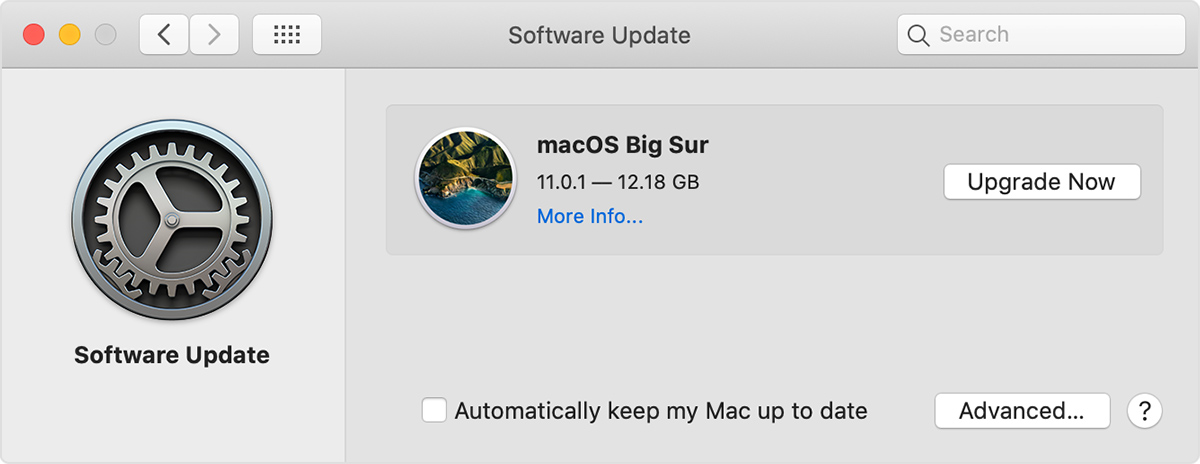
\includegraphics[width=\textwidth]{mac_software_update_app.png}
    \caption{The Windows Update application.}
    \label{fig:mac-update-app}
\end{marginfigure}
\begin{marginfigure}
    \centering
    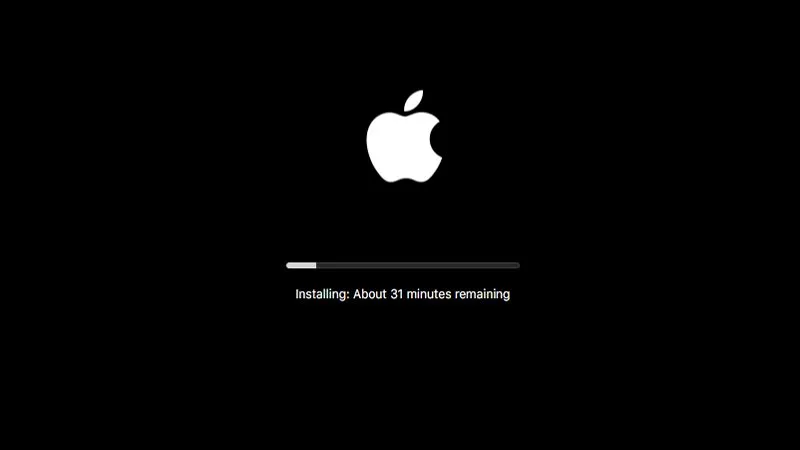
\includegraphics[width=\textwidth]{mac_software_update_screen.png}
    \caption{Your screen while Windows is updating.}
    \label{fig:mac-update-screen}
\end{marginfigure}
\begin{enumerate}[noitemsep,topsep=0pt]
    \item Save all your open documents and close any applications you are not using, including documents and applications that may be minimized or on other spaces.
    \item In the upper-left corner of your screen, select the Apple menu 
\includegraphics[height=.5\baselineskip]{apple_logo.png} and choose ``System Preferences''.
    \item Select ``Software Update'' then ``Update Now'' or ``Upgrade Now''. See Figure~\ref{fig:mac-update-app}.
    \item Wait for the download to complete. This may take a few minutes or longer depending on the speed of your connection and the size of the update.
    \item Select the ``Restart Now'' button. Depending on your security settings, may need to enter your account password. You may be prompted to save and close other applications.
    \item Your computer should partially restart and you will see a black screen with a white Apple logo with a white status bar and time estimate below it. This bar may fill up and your computer may restart again one or more times, this is usually normal. See Figure~\ref{fig:mac-update-screen}.
    \item The update is complete when you are back at the login screen. Log in and check for updates one more time to be sure. If there are no more updates, proceed to the Step 1 section. If there are more updates, install them before proceeding.
\end{enumerate}

\section{I am confused about updating Windows.} If you have a PC running Windows, use the Windows Update application to update Windows to the latest version.\footnote{More details and support can be found on the Windows support site \href{https://support.microsoft.com/en-us/windows/update-windows-10-3c5ae7fc-9fb6-9af1-1984-b5e0412c556a}{here}.} Please note that this step could take 10--30 minutes, maybe longer.
\begin{marginfigure}
    \centering
    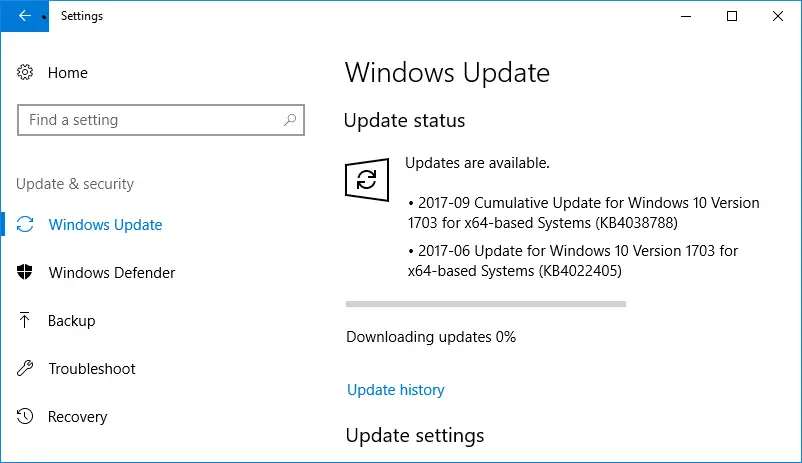
\includegraphics[width=\textwidth]{windows_update_app.png}
    \caption{The Windows Update application.}
    \label{fig:windows-update-app}
\end{marginfigure}
\begin{marginfigure}
    \centering
    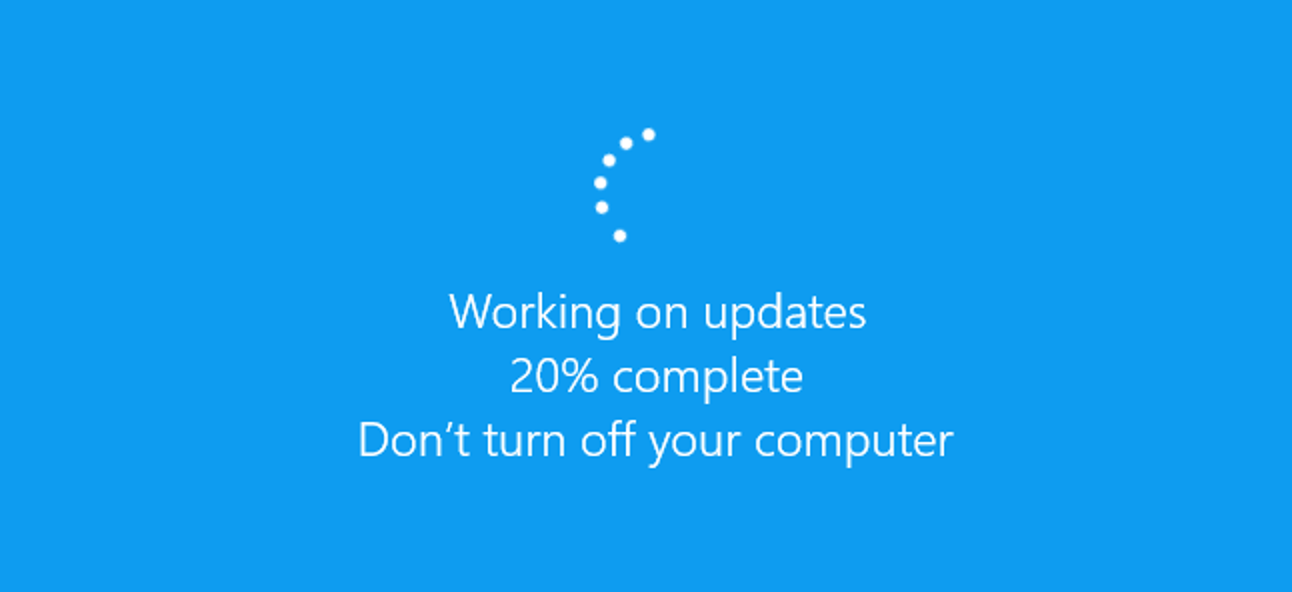
\includegraphics[width=\textwidth]{windows_update_screen.png}
    \caption{Your screen while Windows is updating.}
    \label{fig:windows-update-screen}
\end{marginfigure}

\begin{enumerate}[noitemsep,topsep=0pt]
    \item Save all your open documents and close any applications you are not using, including documents and applications that may be minimized or on other desktops.
    \item Select the Start 
\includegraphics[height=.65\baselineskip]{windows_logo.png} button and go to ``Settings'', ``Update \& Security'', and select ``Windows Update''.
    \item An update may already be waiting. Click the ``Check for updates'' button to check if other updates are queued. See Figure~\ref{fig:windows-update-app}.
    \item Wait for the download to complete. This may take a few minutes or longer depending on the speed of your connection and the size of the update.
    \item Select the ``Restart Now'' button. Depending on your security settings, may need to enter your account password. You may be prompted to save and close other applications.
    \item Your computer should partially restart and you will see a blue screen with a progress indicator. See Figure~\ref{fig:windows-update-screen}.
    \item The update is complete when you are back at the login screen. Log in and check for updates one more time to be sure. If there are no more updates, proceed to the Step 1 section. If there are more updates, install them before proceeding.
\end{enumerate}


% LaTeX Canvas: Chapter Outline
\chapter{Local File System}
\label{ch:filesystem}

\section*{Purpose}
Most beginner frustration in computing is not ``coding’’—it is losing track of files, confusing locations, and breaking workflows by moving or renaming things. This chapter builds durable habits for accessing, navigating, organizing, and managing files and folders on \textbf{Windows} (File Explorer) and \textbf{macOS} (Finder).

\section*{Learning objectives}
By the end of this chapter, a reader should be able to:
\begin{enumerate}
\item Explain the difference between \textbf{files}, \textbf{folders/directories}, \textbf{paths}, and \textbf{extensions}.
\item Navigate reliably in File Explorer and Finder using core affordances (sidebar, breadcrumbs, search, recent, tags).
\item Use absolute vs relative paths and understand key path conventions on Windows and macOS.
\item Adopt naming and organization conventions that scale from one assignment to a multi-month project.
\item Recognize hidden files, sync-folder behaviors (OneDrive/iCloud), and common pitfalls.
\item Apply basic safety practices: avoid destructive moves, manage duplicates, and preserve provenance.
\end{enumerate}

\section*{Running theme: ``Location is a dependency’’}
A script, notebook, or application often assumes files are in specific locations. Good file management makes those dependencies explicit and stable.

\section{A beginner mental model}
\subsection{Files vs folders}
\begin{itemize}
\item \textbf{File:} a named unit of stored data (e.g., \texttt{report.docx}, \texttt{data.csv}).
\item \textbf{Folder/directory:} a container that holds files and other folders.
\item \textbf{Hierarchy:} folders inside folders form a tree.
\end{itemize}

\subsection{Paths: how the computer points to a location}
\begin{itemize}
\item \textbf{Absolute path:} full location from a root.
\item \textbf{Relative path:} location relative to your current folder.
\item \textbf{Separators:} Windows uses backslashes (\texttt{\textbackslash}); macOS uses forward slashes (\texttt{/}).
\end{itemize}

\subsection{Windows vs macOS path conventions (what novices must know)}
\begin{itemize}
\item \textbf{Windows:} drive letters and fully-qualified paths like \texttt{C:\textbackslash Users\textbackslash name\textbackslash Documents}; also network (UNC) paths like \texttt{\textbackslash server \textbackslash share}.
\item \textbf{macOS:} volume-and-directory paths like \texttt{/Users/name/Documents} (POSIX-style).
\item \textbf{Path length and odd edge cases:} Windows has historical maximum path-length constraints and special path forms; you should keep project paths short and avoid deeply nested folders when possible.
\end{itemize}

\subsection{Extensions and file types}
\begin{itemize}
\item Extensions (e.g., \texttt{.csv}, \texttt{.py}) help your OS and apps guess how to open a file.
\item For reproducible work, prefer stable, plain formats (\texttt{.csv}, \texttt{.txt}, \texttt{.md}) over opaque or proprietary formats when possible.
\end{itemize}

\section{Access and navigation on Windows (File Explorer)}
\subsection{Opening and orienting}
\begin{itemize}
\item Open File Explorer; identify the sidebar (Quick access/Home), main pane, and address bar.
\item Learn the breadcrumbs: click segments in the path bar to jump to parent folders.
\end{itemize}

\subsection{Core navigation skills}
\begin{itemize}
\item Move up/down the hierarchy, open in new tabs/windows, and return to recent locations.
\item Use search correctly: search within the current folder vs across the whole machine.
\item Use sort and view options: by name, date modified, type, size.
\end{itemize}

\subsection{Make file extensions and hidden items visible (when troubleshooting)}
\begin{itemize}
\item Toggle viewing extensions to avoid confusion (\texttt{data.csv} vs \texttt{data.csv.txt}).
\item Toggle hidden items when necessary for diagnostics.
\end{itemize}

\subsection{Local vs synced locations (OneDrive)}
\begin{itemize}
\item Understand sync status indicators and what they imply about local availability.
\item Recognize online-only'' vs always keep on this device’’ behaviors, especially when working offline.
\end{itemize}

\section{Access and navigation on macOS (Finder)}
\subsection{Opening and orienting}
\begin{itemize}
\item Open Finder; identify the sidebar (Favorites, iCloud Drive), toolbar, and path location.
\item Understand view modes: icons, list, columns, gallery (choose based on task).
\end{itemize}

\subsection{Core navigation skills}
\begin{itemize}
\item Use the hierarchy: parent folders, column view for rapid browsing.
\item Use Finder search and filters; search this Mac vs this folder.
\item Use tags to create lightweight categories without moving files.
\end{itemize}

\subsection{Hidden files and system folders (what to avoid)}
\begin{itemize}
\item Finder hides some system locations by default; treat hidden/system folders as ``do not edit unless you know why.’’
\item If you must inspect hidden files for troubleshooting, do so carefully and revert the view when done.
\end{itemize}

\subsection{Local vs iCloud behavior}
\begin{itemize}
\item macOS can optimize storage by moving less-used files to iCloud and downloading them on demand.
\item Implication for projects: ensure critical files are actually present locally before running analyses.
\end{itemize}

\section{Organizing work: conventions that scale}
\subsection{A default structure for students}
Recommend a stable home for course work:
\begin{itemize}
\item \texttt{School/} or \texttt{Courses/}
\item \texttt{CourseName/}
\item \texttt{Assignments/}, \texttt{Labs/}, \texttt{Project/}
\end{itemize}

\subsection{A default structure for data projects}
\begin{itemize}
\item \texttt{README.md} (how to run, where things are)
\item \texttt{data/raw/} (immutable inputs)
\item \texttt{data/processed/} (derived outputs)
\item \texttt{src/} (scripts and reusable code)
\item \texttt{notebooks/} (exploration, not production)
\item \texttt{reports/} or \texttt{figures/}
\end{itemize}

\subsection{Naming conventions}
\begin{itemize}
\item Use meaningful, stable names: \texttt{YYYY-MM-DD} prefixes for dated artifacts.
\item Avoid spaces and special characters when files will be used in code.
\item Prefer lowercase with hyphens/underscores: \texttt{clean-survey-2026-01.csv}.
\item Never use \texttt{final.docx}, \texttt{final-final.docx}; use semantic versioning or dates.
\end{itemize}

\subsection{Provenance and duplicates}
\begin{itemize}
\item Keep raw files read-only; do not edit original data in place.
\item When you must create variants, record why and how (notes in README or a changelog).
\item Learn to detect duplicates (same name, different content; same content, different name).
\end{itemize}

\section{Search, metadata, and ``finding it later’’}
\subsection{Search strategies that work}
\begin{itemize}
\item Search by extension (\texttt{.csv}, \texttt{.ipynb}) and by date modified.
\item Use unique keywords in filenames so search works.
\item Use tags (macOS) or pinned/Quick Access folders (Windows) for frequently used locations.
\end{itemize}

\subsection{Sort and view for diagnosis}
\begin{itemize}
\item Sort by date modified to find what changed.
\item View details (size, type) to spot suspicious zero-byte or unexpectedly large files.
\end{itemize}

\section{File operations and safety}
\subsection{Copy vs move vs rename}
\begin{itemize}
\item \textbf{Copy:} duplicates content; safer when experimenting.
\item \textbf{Move:} changes location; can break code/notebooks that reference the old path.
\item \textbf{Rename:} changes identity; can break references and links.
\end{itemize}

\subsection{Delete and recover}
\begin{itemize}
\item Understand Trash/Recycle Bin behavior.
\item Treat permanent deletion as destructive; verify before emptying.
\end{itemize}

\subsection{Permissions basics (just enough)}
\begin{itemize}
\item Errors like Access denied'' or Permission denied’’ usually mean you lack rights to read/write/execute.
\item Prefer working in your user home directory; avoid system directories.
\end{itemize}

\section{Common student pitfalls (and how to avoid them)}
\subsection{Pitfall: working from Downloads/Desktop forever}
\begin{itemize}
\item Symptom: files disappear, duplicates accumulate, paths break.
\item Fix: move projects into a stable \texttt{Courses/} or \texttt{Projects/} location.
\end{itemize}

\subsection{Pitfall: confusing cloud-sync with local storage}
\begin{itemize}
\item Symptom: notebook cannot find data, or files are not available offline.'' \item Fix: confirm local availability; understand sync icons and on demand’’ downloads.
\end{itemize}

\subsection{Pitfall: accidental extension changes}
\begin{itemize}
\item Symptom: file opens in the wrong program or fails to load.
\item Fix: show extensions when working with data/code; avoid manual extension edits unless you understand the effect.
\end{itemize}

\subsection{Pitfall: moving folders after writing code}
\begin{itemize}
\item Symptom: scripts break because paths are hard-coded.
\item Fix: keep a stable project root; use relative paths inside projects.
\end{itemize}

\section{Bridging to the terminal and programming}
\subsection{Why file habits matter for code}
\begin{itemize}
\item Your ``current working directory’’ controls how relative paths resolve.
\item Cross-platform projects should avoid hard-coded, machine-specific absolute paths.
\end{itemize}

\subsection{Cross-platform path handling (conceptual)}
\begin{itemize}
\item Prefer path-join utilities (e.g., language path libraries) rather than manual concatenation.
\item Keep paths short, avoid special characters, and standardize folder structure.
\end{itemize}

\section{Worked examples (outline)}
\subsection{Example 1: Build a course workspace on Windows and macOS}
\begin{itemize}
\item Create the \texttt{Courses/} directory.
\item Create an assignment folder with a consistent template.
\item Pin/favorite the folder for quick access.
\end{itemize}

\subsection{Example 2: Turn a messy Downloads folder into a clean project}
\begin{itemize}
\item Identify project files by extension and date.
\item Move into a new project root.
\item Create \texttt{data/raw} vs \texttt{data/processed} and update references.
\end{itemize}

\subsection{Example 3: Diagnose ``file not found’’}
\begin{itemize}
\item Confirm the file exists, the name matches exactly, and the extension is correct.
\item Confirm you are searching/running from the intended directory.
\item Confirm cloud-sync availability and permissions.
\end{itemize}

\section{Exercises}
\begin{enumerate}
\item Create a project folder structure and explain (in one paragraph) why each folder exists.
\item Rename 10 files using a consistent naming convention; justify the convention.
\item Find all \texttt{.csv} files in your course workspace using OS search.
\item Make a ``raw data is immutable’’ rule: copy raw data, produce processed data, and document the transformation.
\item Break and fix: move a folder referenced by a notebook/script; then repair it using relative paths.
\end{enumerate}

\section{One-page checklist}
\begin{itemize}
\item I know where my project root is.
\item My project uses a consistent folder structure.
\item Raw data is preserved and not edited in place.
\item Filenames are descriptive, stable, and machine-friendly.
\item I can find files by search (extension/date/keyword).
\item I understand whether files are local or cloud-on-demand.
\item I can show extensions/hidden items when troubleshooting and hide them afterward.
\item I avoid working in system directories and respect permissions.
\end{itemize}

\appendix
\section{Reference: key locations (quick map)}
\subsection{Windows (typical)}
\begin{itemize}
\item User home: \texttt{C:\textbackslash Users\textbackslash \textbackslash}
\item Documents/Downloads/Desktop under user home
\item OneDrive folder (if enabled): typically under user home
\end{itemize}

\subsection{macOS (typical)}
\begin{itemize}
\item User home: \texttt{/Users//}
\item Documents/Downloads/Desktop under user home
\item iCloud Drive appears in Finder sidebar; local availability may vary with storage settings
\end{itemize}

Your computer's ``file system'' is the hierarchy of folders and files where programs and documents are saved as well as the software and hardware for storing and retrieving these data. Windows and macOS are very different operating systems with very different underlying file systems. It is really important that you are able to access and navigate through your computer's file system for everything from downloading files to configuring options. This section will cover how to familiarize yourself with your computer's file system, the location of some important folders, and navigating to new folders you create. In this section, you will do this using the graphical user interfaces (GUI) in macOS or Windows.

\begin{marginfigure}
    \centering
    
\includegraphics[width=.65\textwidth]{macos_finder_icon.png}
    \caption{The macOS Finder icon.}
    \label{fig:macos-finder-icon}
\end{marginfigure}

\paragraph{macOS Finder.} The ``Finder'' application is the primary graphical user interface for interacting with the macOS file system.\footnote{\url{https://support.apple.com/en-us/HT201732}}  Finder is always running in the background when you are using macOS.  A few core actions will help you orient yourself:
\begin{enumerate}
    \item \textbf{Open a Finder window.} Click the Finder smiley face icon in the Dock.  If Finder is already active but no window is visible, choose \texttt{File \(\rightarrow\) New Finder Window} from the menu bar or press \texttt{Command\,+\,N}.
    \item \textbf{Navigate via the sidebar.} The sidebar lists common locations (Favorites, iCloud Drive, Downloads, Applications).  Clicking a folder shows its contents in the main pane.  Use the back and forward buttons to move through history.
    \item \textbf{Choose a view.} Use the toolbar buttons or \texttt{View \(\rightarrow\)} menu to switch between icon, list, column, and gallery views.  Column view is especially useful for seeing the folder hierarchy and previewing files without opening them.
    \item \textbf{See the full path.} Enable the path bar via \texttt{View \(\rightarrow\) Show Path Bar}.  You can also right‑click the window title to copy the folder’s full path for use in scripts.
    \item \textbf{Search effectively.} Press \texttt{Command\,+\,F} to search.  Use the scope buttons to limit search to the current folder or your entire Mac, and refine results by kind, date, or name.
\end{enumerate}

\begin{marginfigure}
    \centering
    
\includegraphics[width=.65\textwidth]{windows_explorer_icon.png}
    \caption{The Windows Explorer icon.}
    \label{fig:windows-explorer-icon}
\end{marginfigure}

\paragraph{Windows File Explorer.} Windows File Explorer is the graphical tool for navigating the file system on Windows.  Open it by clicking the folder icon in the taskbar, pressing \texttt{Windows\,+\,E}, or selecting \texttt{File Explorer} from the Start menu.  Key concepts include:
\begin{enumerate}
    \item \textbf{Navigation pane.} The left‑hand pane contains Quick Access (pinned and recent folders), This PC (drives and user folders), and network locations.  Click an entry to display its contents in the main pane.  Pin frequently used folders to Quick Access by right‑clicking and choosing ``Pin to Quick access.''
    \item \textbf{Address bar and breadcrumbs.} The address bar shows your current path as clickable segments (breadcrumbs).  You can type a path (e.g., \texttt{C:\textbackslash Users\textbackslash name\textbackslash Documents}) and press \texttt{Enter} to jump directly.  Right‑click the bar to copy the full path.
    \item \textbf{Views and sorting.} Use the \texttt{View} tab or the layout buttons to switch between details, list, tiles, or large icons.  Sort by name, date modified, type, or size to locate files quickly.
    \item \textbf{Search box.} The search box in the top‑right corner searches within the current folder by default.  Combine it with filters like kind or date (via the Search tab) to narrow results.  Remember that searching the entire drive can take time.
\end{enumerate}

\paragraph{File paths.} A ``file path'' is an address that describes where a folder or file lives on your computer. The file paths for Windows and macOS use different formats and the commands for navigating and accessing each are not compatible. I am going to use my personal Mac and PC computers as an example; the file paths on your computer will be different. My ``Downloads'' folder on my Windows has a file path of \texttt{C:\textbackslash Users\textbackslash Brian\textbackslash Downloads}. The \texttt{C:\textbackslash} is the name of the primary hard drive on almost every PC.\footnote{If you have multiple hard drives, } My ``Downloads'' folder on my macOS has a file path of \texttt{/Users/Brian/Downloads}.

\noindent\textbf{Note on drives and separators.} Windows may assign other drive letters (\texttt{D:}, \texttt{E:}, etc.) if you have multiple hard drives or partitions.  Replace \texttt{C:\textbackslash} with the correct letter when constructing paths.  Also remember that Windows uses backslashes (\texttt{\textbackslash}) to separate path components, whereas macOS and Linux use forward slashes (\texttt{/}).  This difference matters when typing paths in the terminal or code.

\section{Why can't I find a file I downloaded from Canvas? Where did it go?}
Building on the ideas about your computer's file system from the previous section, it is important to know where to find the files we download using our web browser. Depending on the defaults and other preferences of your web browser, downloaded folders might go to your Desktop, a Downloads folder, or some other place. The steps below will make sure that your browser is downloading the folders to a consistent location: your Downloads folder. Instructions for changing the download location of the most popular web browsers (Chrome, Safari, Firefox, and Edge) are listed below with links to their official documentation or other tutorials.

\begin{marginfigure}
    \centering
    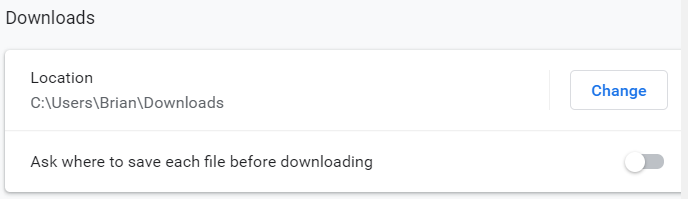
\includegraphics[width=\textwidth]{download-location-chrome.png}
    \caption{Changing the file download location in Chrome.}
    \label{fig:download-location-chrome}
\end{marginfigure}

\paragraph{Chrome.}\hspace{-3pt}\footnote{\url{https://support.google.com/chrome/answer/95759}} Open Chrome, click the 
\includegraphics[height=.65\baselineskip]{hamburger_trail.png} button in the upper right corner, select ``Settings'', and scroll to the bottom and click ``Advanced''. Under the ``Downloads'' section, click ``Change''. Use the Finder (macOS) or File Explorer (Windows) window that pops up to navigate to your ``Downloads'' folder and click ``Select Folder''. See Figure~\ref{fig:download-location-chrome}.

\begin{marginfigure}
    \centering
    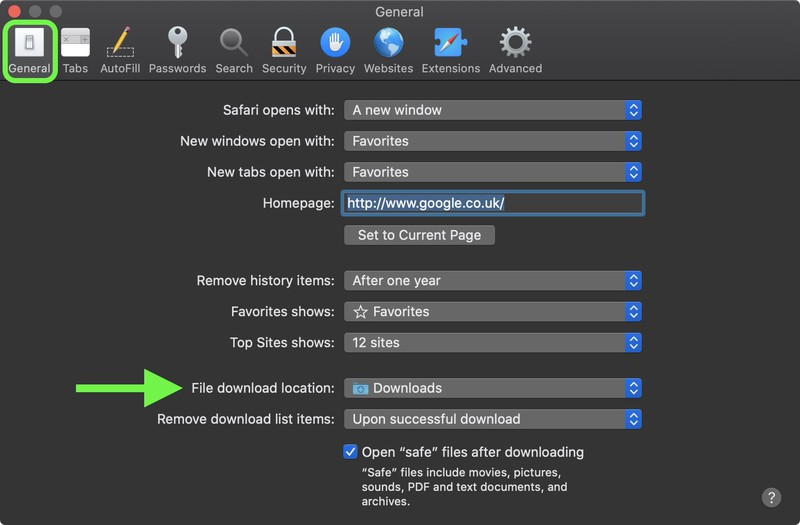
\includegraphics[width=\textwidth]{download-location-safari.png}
    \caption{Changing the file download location in Safari.}
    \label{fig:download-location-safari}
\end{marginfigure}

\paragraph{Safari.}\hspace{-3pt}\footnote{\url{https://www.macrumors.com/how-to/change-safari-download-save-location-mac/}} This should be set to your ``Downloads'' folder by default but here are the steps to change it. Open Safari, select ``Safari'' from the menu bar, and click ``Preferences...''. In the ``General'' tab, click the drop-down next to ``File download location. User the Finder window that pops up to navigate to your ``Downloads'' folder. See Figure~\ref{fig:download-location-safari}.

\paragraph{Mozilla.}\hspace{-3pt}\footnote{\url{https://support.mozilla.org/en-US/kb/where-find-and-manage-downloaded-files-firefox}} Open Firefox, click the 
\includegraphics[height=.65\baselineskip]{hamburger_menu.png} button in the upper-right, and select ``Settings''. In the ``General'' panel, scroll down to the ``Files and Applications'' section, and click the ``Browse...'' button. Use the Finder (macOS) or File Explorer (Windows) window that pops up to navigate to your ``Downloads'' folder and click ``Select Folder''. See Figure~\ref{fig:download-location-mozilla}.

\begin{marginfigure}
    \centering
    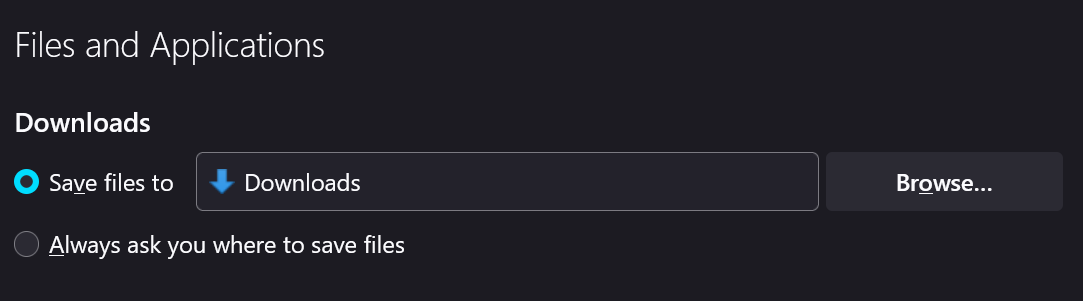
\includegraphics[width=\textwidth]{download-location-mozilla.png}
    \caption{Changing the file download location in Mozilla.}
    \label{fig:download-location-mozilla}
\end{marginfigure}

\paragraph{Edge.}\hspace{-3pt}\footnote{\url{https://support.microsoft.com/en-us/microsoft-edge/change-the-downloads-folder-location-in-microsoft-edge-4049e93b-0ef6-e44f-aca0-7d5f37a39294}} Open Edge, slick the 
\includegraphics[height=.65\baselineskip]{three_dots.png} button in the upper-right, and  click ``Settings''. Select ``Downloads'' in the menu on the left and in the ``Location'' area click the click the ``Change'' button. Use the File Explorer window that pops up to navigate to your ``Downloads'' folder and click ``Select Folder''. See Figure~\ref{fig:download-location-edge}.

\paragraph{File types.} Note that some file types like PDFs may open by default in your web browser rather than saving to your Downloads folder. Some other types of files like DOC or XLS may open in Word or Excel by default and are saved in arcanely-named and impossible-to-find temporary folders. If you want to be able to work with these files after you have downloaded them, make sure to use the ``Save as'' functionality in the browser, PDF reader, Office application, \textit{etc.} to move it to a more appropriate location like a ``Downloads'' or class-specific folder. The details on how to do this are specific to that application: use the documentation links provided for the browsers in the previous section to search for information and tutorials if you are having trouble.

\begin{marginfigure}
    \centering
    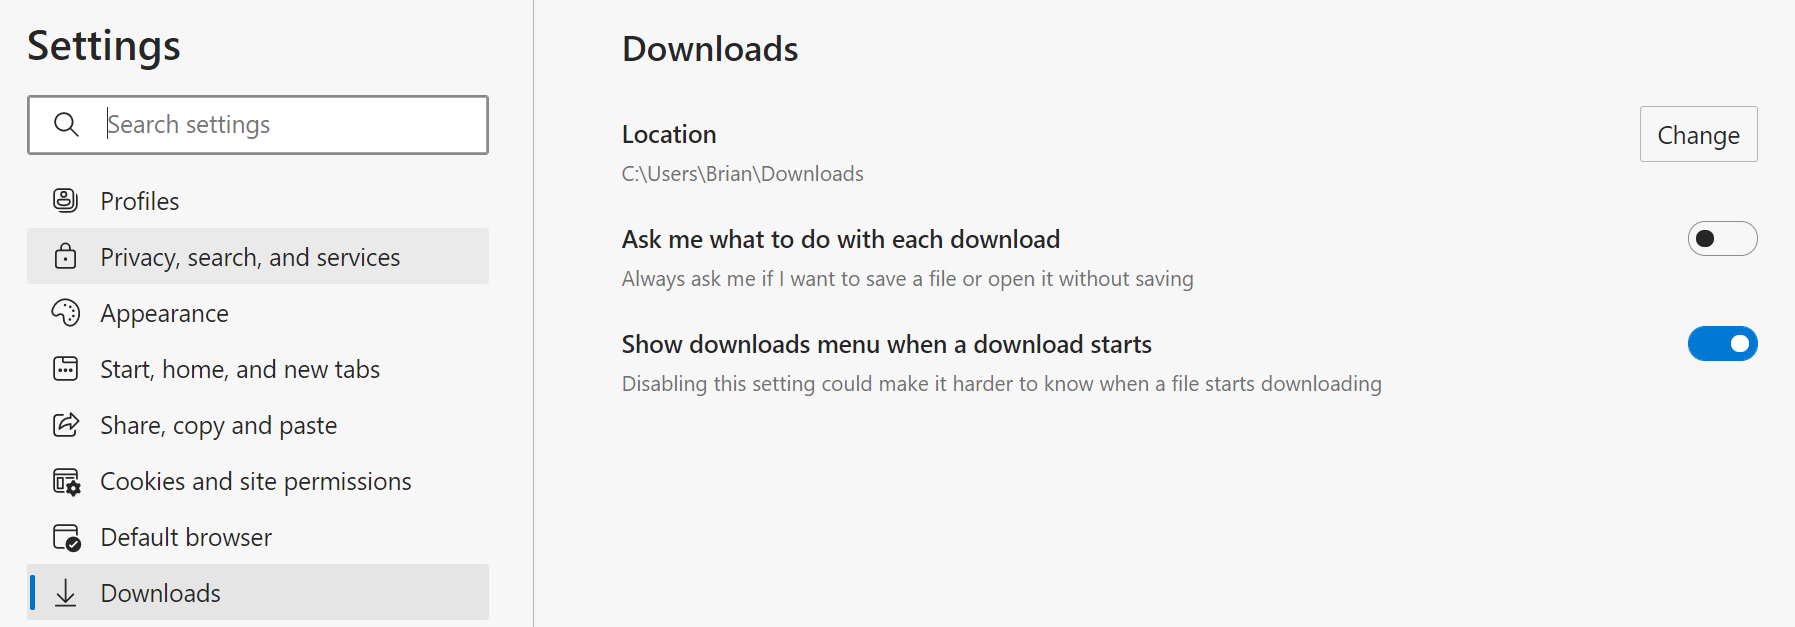
\includegraphics[width=\textwidth]{download-location-edge.png}
    \caption{Changing the file download location in Edge.}
    \label{fig:download-location-edge}
\end{marginfigure}



\section{What does it mean to unzip a file? How do I do that?}

Compressed zip files are archives that bundle one or more files into a single package and reduce their size.  Before you can work with the contents, you need to \emph{unzip} (extract) the archive.  Both Windows and macOS provide built‑in tools to handle zip files, and many third‑party tools exist.  The basic workflow is the same:

\paragraph{On Windows.} Locate the \texttt{.zip} file in File Explorer.  Right‑click the file and choose ``Extract All...'' from the context menu.  A dialog will ask where to extract the files; by default it creates a folder with the same name as the zip file in the current directory.  You can browse to choose a different location.  After extraction completes, open the new folder to access the files.  It is safe to delete the original zip file once you have verified that the extraction succeeded.

\paragraph{On macOS.} Double‑click the \texttt{.zip} file in Finder or select it and choose \texttt{File \(\rightarrow\) Open}.  Archive Utility will automatically decompress the archive into a folder alongside the zip file.  If you need more control, you can right‑click and select ``Open With \(\rightarrow\) Archive Utility'' or use a third‑party app such as The~Unarchiver.  After unzipping, a folder with the same name appears; open it to access the extracted files.  You can move this folder into your project structure and delete the original zip file.

\paragraph{Safety tips.} Never run executables from a zip file you downloaded unless you trust the source.  Always choose a destination folder you can locate easily (for example, your ``Downloads'' folder or a course project folder), and avoid unzipping directly into system folders.  Keep raw zipped archives if you need to preserve the original state for provenance, but otherwise deleting them saves space.
% LaTeX Canvas: Chapter Outline
\chapter{Command Line}
\label{ch:terminal}

\section*{Purpose}
The terminal (command line) is a fast, precise interface for navigating files, running programs, and automating repetitive work. For novices, it can also be intimidating and risky because small mistakes can delete or overwrite work. This chapter builds confident, safe habits for everyday command-line use.

\section*{Learning objectives}
By the end of this chapter, you should be able to:
\begin{enumerate}
\item Explain what a \textbf{terminal} and a \textbf{shell} are, and how commands run.
\item Navigate the file system reliably (absolute/relative paths, current directory).
\item Create, view, copy, move, and delete files and directories safely.
\item Use help tools (\texttt{--help}, \texttt{man}) and interpret usage/syntax.
\item Combine commands with pipes and redirection to build small workflows.
\item Understand exit codes, errors, and common failure messages.
\item Use permissions and \texttt{sudo} responsibly (least privilege, when \emph{not} to use it).
\item Apply basic security hygiene: protect secrets, avoid unsafe pastes, and reduce accidental damage.
\end{enumerate}

\section*{Scope note}
This chapter focuses on Unix-like shells (macOS Terminal, Linux, and Windows via WSL). An appendix maps concepts to Windows PowerShell where relevant.

\section{A beginner mental model}
\subsection{Terminal vs shell}
\begin{itemize}
\item \textbf{Terminal:} the application window you type in.
\item \textbf{Shell:} the command interpreter (often \texttt{bash} or \texttt{zsh}) that runs programs.
\item \textbf{Command:} a program + arguments you ask the shell to run.
\end{itemize}

\subsection{What happens when you press Enter}
\begin{enumerate}
\item The shell reads your command line.
\item It expands shortcuts (globs, variables).
\item It locates the program (via \texttt{PATH}).
\item It runs the program in a process and prints output.
\item It returns an \textbf{exit code}: 0 usually means success.
\end{enumerate}

\subsection{Why the command line matters}
\begin{itemize}
\item High action-to-keystroke ratio (fast for repetitive work).
\item Composability (small tools + pipes).
\item Automation (scripts; reproducible workflows).
\item Remote access (SSH; see Chapter~\ref{ch:remote-computing}).
\end{itemize}

\section{Orientation and safety first}
\subsection{Know where you are (the current working directory)}
\begin{itemize}
\item Use \texttt{pwd} to print the current directory.
\item Use \texttt{ls} to list contents.
\item Use \texttt{cd} to change directories.
\end{itemize}

\subsection{The ``guardrails'' mindset}
\begin{itemize}
\item Prefer \textbf{read-only} commands first: \texttt{pwd}, \texttt{ls}, \texttt{cat}, \texttt{head}.
\item Before destructive actions: do a dry run (list the targets).
\item When in doubt: copy instead of move; move instead of delete.
\end{itemize}

\subsection{Common irreversible mistakes}
\begin{itemize}
\item Deleting the wrong directory (especially with recursive delete).
\item Running a command in the wrong directory.
\item Overwriting files with redirection (\texttt{>}).
\item Using \texttt{sudo} to ``fix'' permission problems without understanding them.
\end{itemize}

\section{Command anatomy and help}
\subsection{Basic syntax}
\begin{verbatim}
command [options] [arguments]
\end{verbatim}

\subsection{Flags and options}
\begin{itemize}
\item Short flags: \texttt{-l}, \texttt{-a}
\item Long flags: \texttt{--all}, \texttt{--help}
\item Some flags take values: \texttt{-o filename} or \texttt{--output=filename}
\end{itemize}

\subsection{Built-in help}
\begin{itemize}
\item \texttt{command --help}
\item \texttt{man command}
\item Skim \texttt{SYNOPSIS} first; then \texttt{OPTIONS}; then \texttt{EXAMPLES}.
\end{itemize}

\subsection{Quoting and spaces}
\begin{itemize}
\item Spaces separate arguments. Use quotes for filenames with spaces.
\item Single quotes usually prevent expansions; double quotes allow some expansions.
\item Rule: quote variables and paths unless you deliberately want splitting/globbing.
\end{itemize}

\section{File system navigation}
\subsection{Key path concepts}
\begin{itemize}
\item \texttt{/} root directory; \texttt{~} your home directory.
\item \texttt{.} current directory; \texttt{..} parent directory.
\item Absolute vs relative paths (Chapter~\ref{ch:filesystem} covers file system organization in depth).
\end{itemize}

\subsection{Core navigation commands}
\begin{itemize}
\item \texttt{pwd} (where am I?)
\item \texttt{ls} (what's here?) and useful flags (\texttt{-l}, \texttt{-a}, \texttt{-h})
\item \texttt{cd} (go there)
\end{itemize}

\subsection{Tab completion and history}
\begin{itemize}
\item Use \textbf{Tab} to complete commands and paths.
\item Use \textbf{Up Arrow} (and reverse search if taught) to reuse commands.
\item Best practice: edit a recalled command instead of retyping.
\end{itemize}

\section{Creating, viewing, and editing files}
\subsection{Creating directories and empty files}
\begin{itemize}
\item \texttt{mkdir} for directories (and \texttt{-p} for nested directories).
\item \texttt{touch} to create a file or update its timestamp.
\end{itemize}

\subsection{Viewing file contents safely}
\begin{itemize}
\item Small files: \texttt{cat}
\item Large files: \texttt{less} (scroll/search)
\item Previews: \texttt{head}, \texttt{tail}
\end{itemize}

\subsection{Creating small files from the command line}
\begin{itemize}
\item Redirection to create simple text files.
\item Prefer a text editor for multi-line content.
\end{itemize}

\subsection{Editors in the terminal}
\begin{itemize}
\item Use a beginner-friendly editor flow (e.g., \texttt{nano}) for quick edits.
\item Know how to exit without panic.
\item For longer-term work, use a full editor (VS Code, etc.).
\end{itemize}

\section{File operations: copy, move, delete (with safety)}
\subsection{Copy and move}
\begin{itemize}
\item \texttt{cp source dest} (copy)
\item \texttt{mv source dest} (move/rename)
\item Use interactive flags where available to prevent overwrites.
\end{itemize}

\subsection{Deleting files and directories}
\begin{itemize}
\item \texttt{rm file} deletes a file.
\item \texttt{rm -r dir} deletes a directory tree.
\item \textbf{High-risk:} \texttt{rm -rf}. Teach why it is dangerous.
\item Safe practice: \texttt{ls} the targets first; consider \texttt{rm -i}.
\end{itemize}

\subsection{Globbing (wildcards) and why it matters}
\begin{itemize}
\item \texttt{*} matches many characters; \texttt{?} matches one.
\item Globs expand \emph{before} the command runs.
\item Safety: run \texttt{echo *.csv} to preview what a glob matches.
\end{itemize}

\section{Searching and inspecting}
\subsection{Finding files}
\begin{itemize}
\item \texttt{find} for locating files by name, type, time.
\item Use carefully; start in a narrow directory scope.
\end{itemize}

\subsection{Searching within files}
\begin{itemize}
\item \texttt{grep} for finding patterns in text.
\item Teach minimal flags: recursive search, case-insensitive search.
\end{itemize}

\subsection{Inspecting file metadata}
\begin{itemize}
\item \texttt{ls -l} for permissions, size, timestamps.
\item \texttt{file} to identify file types.
\item Checksums concept (optional): how to compare transfers.
\end{itemize}

\section{Pipes and redirection: building workflows}
\subsection{Standard streams}
\begin{itemize}
\item \texttt{stdin} (input), \texttt{stdout} (output), \texttt{stderr} (errors).
\end{itemize}

\subsection{Redirection}
\begin{itemize}
\item \texttt{>} overwrite output to a file; \texttt{>>} append.
\item Safety: avoid accidental overwrite; teach creating backups.
\end{itemize}

\subsection{Pipes}
\begin{itemize}
\item \texttt{|} sends output of one command into the next.
\item Common patterns: \texttt{ls | less}, \texttt{grep pattern file | head}.
\end{itemize}

\subsection{Exit codes and ``did it work?''}
\begin{itemize}
\item Teach the idea: commands signal success/failure.
\item Encourage checking outputs, not assuming.
\end{itemize}

\section{Environment basics: \texttt{PATH}, variables, and reproducibility}
\subsection{Environment variables}
\begin{itemize}
\item What they are and why tools use them.
\item Basic operations: \texttt{echo \$VAR}, setting variables (conceptual).
\end{itemize}

\subsection{PATH and locating commands}
\begin{itemize}
\item \texttt{PATH} controls where the shell searches for programs.
\item Use \texttt{which} (or equivalent) to see which program will run.
\item Common pitfall: multiple versions of a tool installed.
\end{itemize}

\subsection{Working directory as a dependency}
\begin{itemize}
\item Relative paths depend on where you run the command.
\item Best practice: adopt a stable project root and use relative paths within it.
\end{itemize}

\section{Permissions, ownership, and \texttt{sudo}}
\subsection{The permission model (just enough)}
\begin{itemize}
\item Users, groups, and ``other.''
\item Read/write/execute bits and what they mean for files vs directories.
\item Recognizing permission errors.
\end{itemize}

\subsection{When to use \texttt{sudo} (and when not to)}
\begin{itemize}
\item \texttt{sudo} runs a single command with elevated privileges.
\item Use it for system-level changes (installing software, editing system configs) when appropriate.
\item Do \textbf{not} use \texttt{sudo} to fix a broken project folder or to run routine scripts.
\end{itemize}

\subsection{Safe \texttt{sudo} practices}
\begin{itemize}
\item Read the command twice before running.
\item Prefer explicit paths over wildcards.
\item Avoid piping into \texttt{sudo} unless you understand the implications.
\item Never run unreviewed copy-pasted commands with \texttt{sudo}.
\end{itemize}

\subsection{Recovering from permission issues}
\begin{itemize}
\item First identify ownership/permissions and the target directory.
\item If you created a mess with \texttt{sudo}, stop and ask for help.
\end{itemize}

\section{Security hygiene for terminal users}
\subsection{Secrets and command history}
\begin{itemize}
\item Your shell history may record commands.
\item Never put passwords/tokens directly on the command line if avoidable.
\item Prefer environment variables, config files with correct permissions, or secret managers (conceptual).
\end{itemize}

\subsection{Copy/paste safety}
\begin{itemize}
\item Understand that copied commands may include hidden characters.
\item Always inspect commands before running; avoid running multi-line scripts you do not understand.
\item Prefer official documentation sources.
\end{itemize}

\subsection{Least privilege}
\begin{itemize}
\item Work in your home directory as a normal user.
\item Elevate privileges only for specific administrative tasks.
\end{itemize}

\section{Workflow patterns for students}
\subsection{Pattern 1: ``enter a project, run, exit''}
\begin{enumerate}
\item \texttt{cd} into a project folder.
\item List files; confirm you are in the right place.
\item Run a command (script, notebook server, tests).
\item Save outputs into a clear directory.
\item Exit cleanly.
\end{enumerate}

\subsection{Pattern 2: creating a reproducible command log}
\begin{itemize}
\item Keep a \texttt{README.md} or \texttt{notes.txt} with the commands needed to reproduce results.
\item Record inputs, outputs, and environment assumptions.
\end{itemize}

\subsection{Pattern 3: safe cleanup}
\begin{itemize}
\item Identify targets with search and preview.
\item Archive important outputs.
\item Delete with care; verify afterward.
\end{itemize}

\section{Troubleshooting playbook}
\subsection{Common errors and what they mean}
\begin{description}
\item[\texttt{command not found}] Program not installed or PATH misconfigured.
\item[\texttt{No such file or directory}] Wrong path, wrong working directory, or typo.
\item[\texttt{Permission denied}] Insufficient rights; avoid reflexive \texttt{sudo}.
\item[\texttt{Is a directory}] Command expected a file.
\end{description}

\subsection{A disciplined response}
\begin{enumerate}
\item Re-run the command slowly; check spelling.
\item Print current directory; list files.
\item Confirm paths and file extensions.
\item Consult \texttt{--help} or \texttt{man}.
\item If still stuck: create a minimal reproduction and ask a precise question.
\end{enumerate}

\section{Worked examples (outline)}
\subsection{Example 1: Build a course workspace}
\begin{itemize}
\item Create directories for \texttt{courses/}, \texttt{assignments/}, \texttt{project/}.
\item Practice navigation and listing.
\end{itemize}

\subsection{Example 2: Create and inspect a dataset file}
\begin{itemize}
\item Download/move a \texttt{.csv}.
\item Preview with \texttt{head} and \texttt{less}.
\item Search for a column name with \texttt{grep}.
\end{itemize}

\subsection{Example 3: Build a small pipeline}
\begin{itemize}
\item Combine commands with pipes.
\item Redirect output to a file.
\item Verify results.
\end{itemize}

\subsection{Example 4: Diagnose and fix a ``file not found'' error}
\begin{itemize}
\item Identify working directory mismatch.
\item Repair using relative paths and project root conventions.
\end{itemize}

\section{Templates}
\subsection{Template A: Safe destructive action checklist}
\begin{verbatim}
Before deleting/moving:

1. pwd
2. ls (confirm context)
3. Preview targets (echo glob / ls targets)
4. Copy/backup if uncertain
5. Execute with least privilege (no sudo unless required)
6. Verify after
   \end{verbatim}

\subsection{Template B: Reproducible command log}
\begin{verbatim}
Project:
Date:
Goal:
Commands:

* ...
  Inputs:
* ...
  Outputs:
* ...
  Notes/assumptions:
* ...
  \end{verbatim}

\section{Exercises}
\begin{enumerate}
\item Navigate from your home directory to a course folder using only \texttt{cd}, \texttt{pwd}, \texttt{ls}.
\item Create a project directory structure with \texttt{mkdir -p}.
\item Create a text file, preview it with \texttt{head}, then open it in \texttt{less}.
\item Copy a directory; rename the copy; explain the difference between copy and move.
\item Use a wildcard to list only \texttt{.csv} files; preview the expansion with \texttt{echo}.
\item Build a pipeline that searches within a file and writes matching lines to an output file.
\item Trigger a permission error intentionally (in a safe location) and explain why \texttt{sudo} is not the first fix.
\end{enumerate}

\section{One-page checklist}
\begin{itemize}
\item I can explain terminal vs shell, and command + arguments.
\item I can navigate with \texttt{pwd}, \texttt{ls}, \texttt{cd} and understand paths.
\item I can create files/directories and view contents safely.
\item I can copy/move/delete with caution and preview wildcards.
\item I can use \texttt{--help} and \texttt{man}.
\item I can use pipes and redirection and understand overwrite vs append.
\item I understand permissions and use \texttt{sudo} only when appropriate.
\item I avoid leaking secrets in commands and history.
\end{itemize}

% \appendix
\section{Windows notes: PowerShell and WSL (optional)}
\subsection{Two common paths}
\begin{itemize}
\item \textbf{WSL} gives a Linux-like shell where \texttt{sudo} and Unix commands apply.
\item \textbf{PowerShell} uses different command names and syntax (but the same mental models: paths, pipes, permissions).
\end{itemize}

\subsection{Concept mapping (high level)}
\begin{itemize}
\item Navigation: \texttt{cd}, \texttt{pwd} (\texttt{Get-Location}), listing (\texttt{ls}/\texttt{dir}).
\item Help: \texttt{--help}/\texttt{man} vs \texttt{Get-Help}.
\item Pipes exist in both, but objects vs text differ.
\end{itemize}


\section{What is a terminal?}

A terminal is a tool for interacting with your computer by issuing commands. A terminal launches a shell (e.g.\ \texttt{bash} or \texttt{zsh}), so sometimes you will hear a ``terminal'' also described as a ``shell''.

\section{What terminal commands should I know, as a basic foundation?}

The exact syntax of terminal commands will be slightly different on Windows and Mac. So to keep things consistent, we are only going to detail high-level descriptions of terminal commands in this guide. 
You can Google the exact commands for your specific system; it is good practice to learn to search for the terminal commands you will need online.

To get started with the terminal for your INFO classes, you should memorize the commands for each of the following: 

\begin{itemize}
\item Activate/deactivate a conda environment
\item Change your directory
\item Install a specific version of a package with conda
\item Inspect the location of a program to the terminal (e.g.\ \texttt{which Python})
\item Print your working directory
\end{itemize}
% LaTeX Canvas: Chapter Outline
\chapter{Text Editors}
\label{ch:text-editors}

\section*{Purpose}
Text editors are the primary tool for writing code, configuring tools, inspecting logs, and fixing small problems quickly. For beginners, the main challenge is not typing---it is developing reliable workflows: opening the right file, editing safely, finding and replacing correctly, and understanding the trade-offs between terminal editors, GUI editors, and full IDEs.

\section*{Learning objectives}
By the end of this chapter, a reader should be able to:
\begin{enumerate}
\item Explain what makes a file ``text'' (vs binary) and why encoding and line endings matter.
\item Use essential editor operations: open/save, undo/redo, find/replace, multi-file search, and navigation.
\item Debug common file problems: wrong path, wrong extension, hidden characters, encoding issues, and line-ending mismatches.
\item Choose an appropriate editor class for a task (terminal editor vs GUI editor vs IDE).
\item Use a GUI editor for simple scripting: run scripts, read errors, and iterate.
\item Apply safe refactoring habits with find/replace and version control.
\item Configure an editor minimally: indentation, formatting, linting, and extensions.
\end{enumerate}

\section*{Running theme: editors are tools, not identities}
Choose an editor that fits the task, and build habits that transfer across editors: paths, file formats, search, safe edits, and reproducibility.

\section{A beginner mental model}
\subsection{Text files are infrastructure}
\begin{itemize}
\item Code, configuration, logs, and data dictionaries are often plain text.
\item Editors are the "workbench" for these artifacts.
\end{itemize}

\subsection{What an editor does (conceptually)}
\begin{itemize}
\item Reads bytes from disk and interprets them as text using an \textbf{encoding} (often UTF-8).
\item Displays text with line breaks and whitespace.
\item Writes bytes back to disk when you save.
\end{itemize}

\subsection{Key terms}
\begin{description}
\item[Encoding] How bytes become characters (UTF-8, etc.).
\item[Line endings] Newline conventions (LF vs CRLF) that affect cross-platform projects.
\item[Whitespace] Spaces/tabs/newlines that can change program behavior.
\item[Syntax highlighting] Visual cues based on language rules.
\item[Linting/formatting] Automated checks and style normalization.
\item[IDE] Integrated Development Environment: editor + build + run + debug + tooling.
\end{description}

\section{Choosing your tool: three editor classes}
\subsection{Terminal editors (nano, vim, emacs)}
\begin{itemize}
\item Best for: remote servers, quick config edits, minimal environments.
\item Strengths: always available, low overhead, works over SSH.
\item Trade-offs: steeper learning curve (especially modal editing), fewer visual affordances.
\item Recommended student baseline: learn \textbf{nano} for emergencies; optionally learn \textbf{vim} motions over time.
\end{itemize}

\subsection{GUI code editors (VS Code, Sublime, etc.)}
\begin{itemize}
\item Best for: daily coursework, scripting, notebooks, lightweight projects.
\item Strengths: search across files, integrated terminal, extensions, formatting, linting.
\item Trade-offs: can become plugin-heavy; configuration drift across machines.
\item Recommended student default: choose one primary GUI editor and learn it well.
\end{itemize}

\subsection{IDEs (Visual Studio, Eclipse, Xcode, etc.)}
\begin{itemize}
\item Best for: large language ecosystems and complex build systems (Java, C\#, Swift, etc.).
\item Strengths: deep refactoring, project models, integrated debugging/build tooling.
\item Trade-offs: heavier setup; more concepts up front; project configuration can be fragile.
\end{itemize}

\subsection{A decision table (student version)}
\begin{itemize}
\item \textbf{Quick edit on a remote server:} terminal editor.
\item \textbf{Python scripting + small projects:} GUI editor.
\item \textbf{Course uses a specific ecosystem (e.g., Java/C\#/iOS):} IDE.
\item \textbf{When unsure:} GUI editor with an integrated terminal.
\end{itemize}

\section{Essential editor skills (transfer across tools)}
\subsection{Open, save, and "where did it go?"}
\begin{itemize}
\item Always know the \textbf{file path} you are editing.
\item Understand "Save" vs "Save As".
\item Recognize read-only files and permission prompts.
\item Build a habit: confirm the directory and filename after saving.
\end{itemize}

\subsection{Undo/redo and safe experimentation}
\begin{itemize}
\item Undo is your first safety net; version control is your second.
\item Save small, frequent changes; keep commits focused.
\end{itemize}

\subsection{Indentation and whitespace}
\begin{itemize}
\item Choose a consistent indentation style for a project.
\item Configure your editor to show or make visible whitespace when debugging.
\item Understand tabs vs spaces and why Python cares.
\end{itemize}

\subsection{Find, replace, and refactoring safety}
\begin{itemize}
\item Use "Find" before "Replace".
\item Prefer "Replace with confirmation" for nontrivial changes.
\item Learn scope: current selection, current file, entire workspace.
\item Learn regular expressions (basic level): anchors, wildcards, capture groups.
\item After replacing: run tests or re-run the script.
\end{itemize}

\subsection{Multi-file search and navigation}
\begin{itemize}
\item Use workspace search to locate symbols and strings.
\item Learn quick navigation: go to file, go to line, go to definition.
\item Keep a mental model of your project root.
\end{itemize}

\section{Simple scripting workflows in an editor (novice level)}
\subsection{Write-run-read-repeat loop}
\begin{enumerate}
\item Write a small script (10--50 lines).
\item Run it from the integrated terminal.
\item Read the error message carefully.
\item Jump to the referenced file/line.
\item Make one change at a time and re-run.
\end{enumerate}

\subsection{Editor features that help beginners}
\begin{itemize}
\item Syntax highlighting and bracket matching.
\item Auto-indentation and formatting-on-save.
\item Linting messages as "early warnings".
\item Inline documentation (hover tooltips) and jump-to-definition.
\end{itemize}

\subsection{When a full debugger helps}
\begin{itemize}
\item Use a debugger when print/logging is too slow or you need to inspect state.
\item Learn the minimum: breakpoints, step over/into, variable inspection.
\end{itemize}

\section{Debugging files (common student failure modes)}
\subsection{Wrong file, wrong place}
\begin{itemize}
\item Symptom: edits do not change program behavior.
\item Cause: you edited a duplicate file or ran from a different directory.
\item Fix: confirm the working directory; search for duplicates; use absolute paths temporarily.
\end{itemize}

\subsection{Wrong extension or hidden extension}
\begin{itemize}
\item Symptom: file opens in the wrong program or fails to run.
\item Fix: show file extensions; confirm \texttt{.py}, \texttt{.csv}, \texttt{.txt}.
\end{itemize}

\subsection{Encoding and invisible characters}
\begin{itemize}
\item Symptom: weird symbols, parsing errors, or "invalid character" errors.
\item Fix: re-save as UTF-8; inspect for non-printing characters; normalize line endings.
\end{itemize}

\subsection{Line endings (Windows/macOS collaboration)}
\begin{itemize}
\item Symptom: scripts fail, diffs look huge, or tools complain about CRLF/LF.
\item Fix: configure editor to use consistent line endings; rely on repo configuration if provided.
\end{itemize}

\subsection{Config files and indentation-sensitive formats}
\begin{itemize}
\item YAML and similar formats can break with tabs or incorrect indentation.
\item Use visible whitespace; validate with the tool that reads the config.
\end{itemize}

\section{Terminal editors: survival skills}
\subsection{nano essentials (minimum viable)}
\begin{itemize}
\item Open, save, exit without panic.
\item Search and replace.
\item Go to line number.
\end{itemize}

\subsection{vim essentials (minimum viable)}
\begin{itemize}
\item Modes: normal vs insert; how to get back to normal.
\item Save and quit.
\item Search and substitute (with confirmation).
\item Why vim feels fast: motions + operators (optional preview).
\end{itemize}

\subsection{emacs essentials (minimum viable)}
\begin{itemize}
\item Open/save/exit.
\item Search.
\item Basic multi-buffer navigation.
\end{itemize}

\section{GUI editors: practical configuration (keep it minimal)}
\subsection{The minimal settings that matter}
\begin{itemize}
\item Indentation and whitespace display.
\item Format on save (using a formatter appropriate to your language).
\item A linter for early feedback.
\item Integrated terminal.
\end{itemize}

\subsection{Extensions/plugins: a controlled approach}
\begin{itemize}
\item Install only what you can explain.
\item Prefer widely used, well-maintained extensions.
\item Avoid overlapping extensions that fight each other.
\item Document your essential extensions for reproducibility.
\end{itemize}

\subsection{Workspace settings vs global settings}
\begin{itemize}
\item Use workspace settings for project-specific behavior.
\item Keep global settings simple so you can reproduce work on another machine.
\end{itemize}

\section{IDEs: fundamentals without overwhelm}
\subsection{Project model}
\begin{itemize}
\item IDEs often manage build configuration, dependencies, and run targets.
\item Learn where the IDE stores project settings and how to reset or re-import.
\end{itemize}

\subsection{Refactoring and code navigation}
\begin{itemize}
\item IDE refactors are powerful but must be reviewed.
\item Always run tests/build after refactors.
\end{itemize}

\subsection{Debugging integration}
\begin{itemize}
\item IDEs make breakpoints and stepping easy.
\item Learn the minimum and rely on it when print-debugging is not enough.
\end{itemize}

\section{Best practices: habits that prevent pain}
\subsection{Pick a primary editor and a fallback}
\begin{itemize}
\item Primary: your daily GUI editor or required IDE.
\item Fallback: nano (and optionally vim) for remote/emergency edits.
\end{itemize}

\subsection{Treat find/replace as a ``power tool"}
\begin{itemize}
\item Narrow scope.
\item Preview changes.
\item Make a commit before large replacements.
\item Verify with tests or a run.
\end{itemize}

\subsection{Keep text files boring}
\begin{itemize}
\item Use UTF-8.
\item Normalize line endings.
\item Avoid editing generated files by hand.
\item Prefer configuration in version control.
\end{itemize}

\subsection{Use version control as an editor safety net}
\begin{itemize}
\item Commit logical steps.
\item Use diffs to review changes before running.
\item Revert when experiments go wrong.
\end{itemize}

\section{Worked examples (outline)}
\subsection{Example 1: Write and run a tiny script}
\begin{itemize}
\item Create \texttt{hello.py}.
\item Run from the terminal.
\item Fix a syntax error using the editor's line/column cues.
\end{itemize}

\subsection{Example 2: Debug a broken config file}
\begin{itemize}
\item Identify indentation and invisible-character issues.
\item Turn on visible whitespace.
\item Validate by re-running the tool.
\end{itemize}

\subsection{Example 3: Safe rename/refactor with find/replace}
\begin{itemize}
\item Use multi-file search.
\item Replace with confirmation.
\item Run tests.
\end{itemize}

\subsection{Example 4: Remote emergency edit over SSH}
\begin{itemize}
\item Open a config file in nano.
\item Make a minimal change.
\item Save/exit; verify.
\end{itemize}

\section{Templates}
\subsection{Template A: Editor setup checklist (first week)}
\begin{verbatim}
Editor:

* Installed and updated
* Default indentation configured
* Visible whitespace toggle known
* Format-on-save configured (if course uses it)
* Linter installed (if course uses it)
* Integrated terminal enabled
  Fallback editor:
* nano basics practiced (open/save/exit/search)
  \end{verbatim}

\subsection{Template B: Safe find/replace protocol}
\begin{verbatim}

1. Search (no replace) and inspect matches
2. Narrow scope (file/selection/project)
3. Replace with confirmation
4. Save and review diff
5. Run tests or rerun script
6. Commit with a message describing the change
   \end{verbatim}

\section{Exercises}
\begin{enumerate}
\item Configure your editor to show line numbers and visible whitespace; explain what you changed.
\item Write a short script and fix two intentional errors using editor cues.
\item Perform a multi-file search in a small project; report where a function name appears.
\item Run a safe find/replace with confirmation and verify by running tests.
\item Open and edit a file in nano; save and exit confidently.
\item Optional: learn a minimal vim workflow (insert, save, quit, search).
\end{enumerate}

\section{One-page checklist}
\begin{itemize}
\item I can open, save, and locate files reliably.
\item I can use find/replace safely, including across multiple files.
\item I can debug common file issues (paths, extensions, encoding, line endings).
\item I understand when to use terminal editors vs GUI editors vs IDEs.
\item My editor is minimally configured (indentation, formatting, linting).
\item I use version control to review and recover from editing mistakes.
\item I have a fallback editor skill for remote/emergency use.
\end{itemize}

\appendix
\section{Quick reference: terminal editor survival commands (optional handout)}
\subsection{nano}
\begin{itemize}
\item Open: \texttt{nano file}
\item Save: (document the keystroke)
\item Exit: (document the keystroke)
\item Find/replace: (document the keystroke)
\end{itemize}

\subsection{vim}
\begin{itemize}
\item Insert mode: \texttt{i}
\item Normal mode: \texttt{Esc}
\item Save/quit: \texttt{:wq}
\item Quit without saving: \texttt{:q!}
\item Search: \texttt{/pattern}
\item Substitute (conceptual): \texttt{:%s/old/new/gc}
\end{itemize}

\section{Quick reference: GUI/IDE search}
\begin{itemize}
\item Find in file, replace in file
\item Find in workspace, replace in workspace
\item Go to line, go to file, go to definition
\end{itemize}

% LaTeX Canvas: Chapter Outline
\chapter{Remote Computing}
\label{ch:remote-computing}

\section*{Purpose}
Remote computing lets you use resources that are not physically on your laptop: university servers, high-performance clusters, lab machines, and cloud instances. This chapter teaches novices how to connect safely and reliably using SSH and VPNs, move files, run remote jobs, and use tunneling to access remote services (including Jupyter) as if they were local.

\section*{Learning objectives}
By the end of this chapter, you should be able to:
\begin{enumerate}
\item Explain client/server basics and what ``remote computing'' means.
\item Use SSH to connect to a remote machine and run commands interactively.
\item Use key-based authentication safely (generate keys, protect private keys, manage known hosts).
\item Transfer files with \texttt{scp} or \texttt{sftp} (and understand when to use GUI tools).
\item Use SSH tunneling (local, remote, and dynamic forwarding) for safe access to remote services.
\item Understand what a VPN does, when it is required, and common pitfalls.
\item Describe cloud computing at a practical level (instances, regions, networking rules, costs).
\item Apply baseline security practices: least privilege, MFA, key hygiene, and avoiding data leaks.
\end{enumerate}

\section*{Running theme: remote access is powerful, so make it boring}
The goal is not cleverness; it is predictable workflows that minimize risk.

\section{A beginner mental model}
\subsection{Local vs remote}
\begin{itemize}
\item \textbf{Local machine:} your laptop/desktop.
\item \textbf{Remote machine:} a computer you access over the network.
\item \textbf{Network:} the path between them (campus, home Wi-Fi, internet).
\end{itemize}

\subsection{Client/server language}
\begin{itemize}
\item \textbf{Client:} the tool you run locally (SSH client, VPN client, browser).
\item \textbf{Server:} the remote service or machine you connect to (SSH server, web server).
\end{itemize}

\subsection{Sessions, processes, and persistence}
\begin{itemize}
\item A remote \textbf{SSH session} is a connection + a shell.
\item Programs you start remotely may stop when your session ends unless you use job control tools.
\item Remote computers have their own file system, users, permissions, and installed software.
\end{itemize}

\subsection{Why remote computing exists}
\begin{itemize}
\item Access to more CPU/RAM/GPU.
\item Access to shared datasets and licensed tools.
\item Reliability (servers run longer than laptops).
\item Collaboration (shared environments).
\end{itemize}

\section{Prerequisites and safe defaults}
\subsection{Accounts and credentials}
\begin{itemize}
\item You need: a username, a host address, and an authentication method.
\item Prefer: institutional identity + MFA, and key-based SSH.
\end{itemize}

\subsection{Install/locate your tools}
\begin{itemize}
\item \textbf{macOS:} Terminal includes \texttt{ssh}, \texttt{scp}, \texttt{sftp}.
\item \textbf{Windows:} OpenSSH client is commonly available; otherwise enable/install it.
\item Optional: a code editor that supports remote development.
\end{itemize}

\subsection{Golden safety rules}
\begin{itemize}
\item Never share passwords or private keys.
\item Never paste secrets into commands or notebooks.
\item Assume your command history is readable by future you (and sometimes by administrators).
\item Use the minimum access needed; log out when done.
\end{itemize}

\section{SSH fundamentals}
\subsection{What SSH provides}
\begin{itemize}
\item Encrypted remote login.
\item Secure file transfer.
\item Secure tunneling of other network traffic.
\end{itemize}

\subsection{The simplest connection}
\begin{verbatim}
ssh username@hostname
\end{verbatim}
\begin{itemize}
\item You may need \texttt{-p <port>} if SSH uses a nonstandard port.
\item The first time you connect, SSH will ask about the host fingerprint.
\end{itemize}

\subsection{Host identity and \texttt{known\_hosts}}
\begin{itemize}
\item SSH remembers server fingerprints to prevent ``man-in-the-middle'' attacks.
\item Warning: a changed fingerprint may be benign (server rebuilt) or dangerous (impersonation).
\item Best practice: verify changes via a trusted channel (course staff / sysadmin).
\end{itemize}

\subsection{Authentication: passwords vs keys}
\begin{itemize}
\item \textbf{Password:} easy to start, less secure, often disabled on managed servers.
\item \textbf{Keys:} recommended; a private key stays on your device and proves identity.
\end{itemize}

\subsection{Key-based authentication basics}
\begin{itemize}
\item A key pair: \textbf{private key} (secret) + \textbf{public key} (shareable).
\item The public key is added to the server's authorized keys list.
\item Protect the private key with a passphrase.
\end{itemize}

\subsection{Generating a key pair (conceptual)}
\begin{verbatim}
ssh-keygen
\end{verbatim}
\begin{itemize}
\item Choose a strong passphrase.
\item Store keys in the default \texttt{~/.ssh/} location.
\item Keep your private key file permissions restrictive.
\end{itemize}

\subsection{SSH agent (optional but useful)}
\begin{itemize}
\item An agent holds decrypted keys in memory so you do not type your passphrase repeatedly.
\item Treat agent forwarding as advanced; do not enable it by default.
\end{itemize}

\subsection{Quality-of-life: \texttt{~/.ssh/config}}
\begin{itemize}
\item Create short nicknames for hosts.
\item Store per-host usernames, ports, and identity files.
\item Keep configuration readable; document nonstandard choices.
\end{itemize}

\section{File transfer: getting data in and out}
\subsection{The basic question: where is the file?}
\begin{itemize}
\item `Local path'' (your computer) vs `remote path'' (server).
\item Use absolute paths if you are unsure.
\end{itemize}

\subsection{Secure copy (\texttt{scp})}
\begin{itemize}
\item Good for quick transfers and scripts.
\item Learn directory copies (recursive) and quoting paths with spaces.
\end{itemize}

\subsection{SFTP (\texttt{sftp})}
\begin{itemize}
\item Interactive file transfer session.
\item Many GUI tools use SFTP under the hood.
\end{itemize}

\subsection{What not to do}
\begin{itemize}
\item Do not email datasets or copy them into unapproved cloud storage.
\item Do not move large files through a slow interactive session if a better transfer method exists.
\end{itemize}

\section{Tunneling and port forwarding (making remote services usable)}
\subsection{Why tunneling exists}
\begin{itemize}
\item Many services (Jupyter, databases, dashboards) bind to \texttt{localhost} on the server for safety.
\item A tunnel lets your local machine reach that service through an encrypted channel.
\end{itemize}

\subsection{Local forwarding (most common)}
\begin{itemize}
\item Scenario: remote server runs a service on \texttt{127.0.0.1:8888}; you want to open it in your local browser.
\end{itemize}
\begin{verbatim}
ssh -L 8888:localhost:8888 username@hostname
\end{verbatim}
\begin{itemize}
\item Then visit \texttt{[http://localhost:8888}](http://localhost:8888) in your local browser.
\item If \texttt{8888} is taken locally, choose another local port (e.g., 8899).
\end{itemize}

\subsection{Remote forwarding (advanced)}
\begin{itemize}
\item Scenario: you need the remote machine to reach a service running locally.
\item Use cautiously; it changes the exposure model.
\end{itemize}

\subsection{Dynamic forwarding (SOCKS proxy)}
\begin{itemize}
\item Scenario: route a browser or tool through the remote network.
\item Use only when you understand policies and implications.
\end{itemize}

\subsection{Tunnel hygiene}
\begin{itemize}
\item Use \texttt{-N} when you only need forwarding (no remote shell).
\item Prefer binding to \texttt{localhost} on your machine to avoid exposing ports to others.
\item Close tunnels when you are done.
\end{itemize}

\section{VPN fundamentals}
\subsection{What a VPN does (student-relevant)}
\begin{itemize}
\item Creates a secure network path to a private network (campus/lab).
\item Makes your device behave as if it is ``on campus'' for protected resources.
\item Often required to reach SSH hosts that are not publicly reachable.
\end{itemize}

\subsection{When you need a VPN}
\begin{itemize}
\item Accessing university resources from off campus.
\item Using internal-only hosts, file shares, or licensed services.
\item Connecting to a protected cluster login node.
\end{itemize}

\subsection{Common VPN pitfalls}
\begin{itemize}
\item VPN drops cause SSH disconnections.
\item Split-tunneling vs full-tunneling changes which traffic goes through the VPN.
\item Some VPNs interfere with local networking (printers, local dev servers).
\end{itemize}

\subsection{Practical advice}
\begin{itemize}
\item Connect VPN first, then SSH.
\item If you lose connection, reconnect VPN and re-establish SSH; do not assume remote processes survived.
\item Learn where your VPN client shows connection status and logs.
\end{itemize}

\section{Remote work patterns: from simple to professional}
\subsection{Pattern 1: login node + compute node (HPC concept)}
\begin{itemize}
\item You SSH into a \textbf{login node} for editing and job submission.
\item Actual computation runs on separate nodes via a scheduler.
\item Rule: do not run heavy jobs on login nodes.
\end{itemize}

\subsection{Pattern 2: remote development}
\begin{itemize}
\item Edit locally and run remotely, or edit remotely using a remote extension.
\item Keep projects in version control; avoid manual copying back and forth.
\end{itemize}

\subsection{Pattern 3: notebooks on servers}
\begin{itemize}
\item Start Jupyter remotely.
\item Use SSH local port forwarding to access it.
\item Prefer passwords/tokens and binding to \texttt{localhost}.
\end{itemize}

\section{Cloud computing basics (what novices must know)}
\subsection{What ``the cloud'' is}
\begin{itemize}
\item Renting computing resources (virtual machines, storage, managed services).
\item You control enough to break things, including security.
\end{itemize}

\subsection{Core terms}
\begin{description}
\item[Instance/VM] A rented computer.
\item[Region/zone] Where the machine physically resides.
\item[Storage] Object storage (buckets) vs attached disks.
\item[Networking rules] Firewalls/security groups controlling inbound/outbound.
\end{description}

\subsection{A safe ``first cloud VM'' workflow}
\begin{enumerate}
\item Create the instance in a region.
\item Create or choose an SSH key pair.
\item Configure inbound access: allow SSH only from your IP (not from the whole internet).
\item Connect via SSH.
\item Shut down/terminate when finished to control cost.
\end{enumerate}

\subsection{Cost and risk}
\begin{itemize}
\item Cloud resources cost money while running (and sometimes while stored).
\item Set budget alerts if available.
\item Do not expose services publicly unless required and reviewed.
\end{itemize}

\section{Security best practices for remote computing}
\subsection{Key hygiene}
\begin{itemize}
\item Use passphrases; do not store private keys in shared folders.
\item Avoid key sprawl: use separate keys per purpose if required, and retire unused keys.
\item If a key might be compromised, rotate it immediately.
\end{itemize}

\subsection{Least privilege and separation}
\begin{itemize}
\item Use non-admin accounts for daily work.
\item Use sudo/admin only when necessary.
\item Keep data access minimal and policy-compliant.
\end{itemize}

\subsection{Safe networking defaults}
\begin{itemize}
\item Restrict inbound ports (SSH only; no public databases).
\item Prefer tunnels over opening ports.
\item Keep software patched on remote machines.
\end{itemize}

\subsection{Logging and traceability (student level)}
\begin{itemize}
\item Keep a small ``remote session log'': what host, what you did, what changed.
\item Use version control for code changes.
\end{itemize}

\section{Troubleshooting and diagnostics}
\subsection{Connection failures}
\begin{itemize}
\item Check: internet, VPN status, host name, username.
\item Check: port and firewall rules.
\item Check: key permissions and correct key selection.
\end{itemize}

\subsection{Host key warnings}
\begin{itemize}
\item Do not ignore.
\item Verify with a trusted source before accepting changes.
\end{itemize}

\subsection{Timeouts and unstable connections}
\begin{itemize}
\item Use keep-alives if permitted.
\item Prefer running long tasks via schedulers or detached sessions.
\end{itemize}

\subsection{``Permission denied''}
\begin{itemize}
\item It may be the wrong username.
\item It may be the wrong key.
\item It may be a server-side access control issue.
\end{itemize}

\section{Worked examples (outline)}
\subsection{Example 1: First SSH login}
\begin{itemize}
\item Verify prerequisites (account, host, VPN).
\item Connect and interpret the login banner.
\item Navigate remote directories and run a simple command.
\end{itemize}

\subsection{Example 2: Move a dataset to a server}
\begin{itemize}
\item Identify local and remote paths.
\item Transfer with \texttt{scp} or \texttt{sftp}.
\item Verify integrity (file size, checksums if taught).
\end{itemize}

\subsection{Example 3: Remote Jupyter via SSH tunnel}
\begin{itemize}
\item Start Jupyter on the server bound to \texttt{localhost}.
\item Create a local tunnel.
\item Connect in browser; close tunnel when done.
\end{itemize}

\subsection{Example 4: Launch and secure a small cloud VM}
\begin{itemize}
\item Create instance; restrict inbound SSH to your IP.
\item SSH in; run a short job.
\item Terminate instance; confirm costs stop accruing.
\end{itemize}

\section{Exercises}
\begin{enumerate}
\item Generate an SSH key pair with a passphrase and identify where keys are stored.
\item Create an \texttt{~/.ssh/config} entry for a host and connect using the alias.
\item Transfer a directory of files to a server and verify the transfer.
\item Create a local port forward and access a remote service in your browser.
\item Connect to a required campus resource through a VPN and note how your network behavior changes.
\item Cloud practice (if allowed): launch a VM, SSH in, then shut it down and confirm termination.
\end{enumerate}

\section{One-page checklist}
\begin{itemize}
\item I know whether I need a VPN before SSH.
\item I can state: username, hostname, and authentication method.
\item My private key is protected (passphrase, correct permissions, not shared).
\item I understand host key prompts and do not ignore warnings.
\item I can transfer files securely and verify destination paths.
\item I can set up a local SSH tunnel for remote services.
\item I restrict network exposure (no unnecessary public ports).
\item I log out and terminate cloud resources when finished.
\end{itemize}

% \appendix
\section{Quick reference: common SSH commands}
\begin{verbatim}
ssh username@hostname
ssh -p 2222 username@hostname
ssh -i ~/.ssh/my_key username@hostname
ssh -L 8888:localhost:8888 username@hostname
scp localfile username@hostname:/remote/path/
sftp username@hostname
\end{verbatim}

\section{Quick reference: vocabulary}
\begin{description}
\item[SSH] Secure Shell protocol for encrypted remote access.
\item[VPN] Virtual Private Network; encrypted connection to a private network.
\item[Tunnel/Port forward] Using SSH to carry traffic for another service.
\item[Public key] Shareable key used by the server to verify the corresponding private key.
\item[Private key] Secret key that proves your identity; must be protected.
\item[Host key] Server identity fingerprint stored in \texttt{known_hosts}.
\item[Security group/firewall] Rules controlling allowed inbound/outbound network traffic.
\end{description}

\part{Python Management}

% LaTeX Canvas: Chapter Outline
\chapter{Package Management}
\label{ch:pkg-mgmt}

\section*{Purpose}
Package management is the discipline of installing and updating third-party software (libraries) in a way that is consistent, reproducible, and unlikely to break your work. For novices, the most common failure mode is mixing global installs, different Python interpreters, and ad-hoc updates until nothing imports. This chapter teaches a stable workflow using project-level environments, clear dependency records, and a conflict-resolution playbook.

\section*{Learning objectives}
By the end of this chapter, a reader should be able to:
\begin{enumerate}
\item Explain what a \textbf{package}, \textbf{dependency}, and \textbf{environment} are.
\item Choose between \texttt{conda} and \texttt{pip} for a given situation.
\item Create, activate, and remove isolated environments (conda environments and/or \texttt{venv}).
\item Install packages with good hygiene (no `random global installs'', avoid base/root env).
  \item Record dependencies for reproducibility (\texttt{environment.yml}, \texttt{requirements.txt}, optional lockfiles).
  \item Diagnose `it worked yesterday'' failures: wrong interpreter, wrong environment, conflicts.
\item Resolve dependency conflicts using solver output, pinning, and environment recreation.
\item Apply maintenance practices: updates, audits, and cleaning without breaking environments.
\end{enumerate}

\section*{Running theme: environments are disposable, projects are not}
Your project should be stable because it describes what it needs. If an environment breaks, you should be able to recreate it.

\section{Mental models and vocabulary}
\subsection{Packages and dependencies}
\begin{itemize}
\item \textbf{Package:} third-party code you install (e.g., \texttt{pandas}).
\item \textbf{Dependency:} another package your package needs.
\item \textbf{Version constraints:} rules like \texttt{>=}, \texttt{<}, \texttt{==} that restrict compatible versions.
\end{itemize}

\subsection{Environments and interpreters}
\begin{itemize}
\item A Python \textbf{interpreter} runs your code (and determines where packages are installed).
\item An \textbf{environment} is an isolated set of installed packages tied to a specific interpreter.
\item You can have many environments on one computer; each project should use one.
\end{itemize}

\subsection{Reproducibility artifacts}
\begin{itemize}
\item \texttt{environment.yml}: conda-style environment specification.
\item \texttt{requirements.txt}: pip-style install list.
\item \textbf{Lockfile:} a fully resolved, exact list of versions for repeatable installs.
\end{itemize}

\section{Choosing tools: \texttt{conda} vs \texttt{pip} vs \texttt{venv}}
\subsection{What conda is good at}
\begin{itemize}
\item Cross-language, compiled dependencies (e.g., scientific stacks, system libraries).
\item Environments that include non-Python packages.
\item Solving complex dependency graphs across compiled packages.
\end{itemize}

\subsection{What pip is good at}
\begin{itemize}
\item Installing Python packages from PyPI.
\item Lightweight environments using the standard library \texttt{venv}.
\item Working with Python packaging metadata (\texttt{pyproject.toml}, wheels).
\end{itemize}

\subsection{Practical student guidance}
\begin{itemize}
\item If your course provides a conda environment file, use conda.
\item If a library is only on PyPI, use pip (inside an environment).
\item Do not install packages globally for coursework.
\end{itemize}

\section{Baseline hygiene rules (non-negotiable)}
\subsection{Rule 1: never work in the base/root conda environment}
\begin{itemize}
\item Keep base/root for conda itself.
\item Create a separate environment per project.
\end{itemize}

\subsection{Rule 2: one project, one environment}
\begin{itemize}
\item Avoid ``one giant environment for everything''.
\item Name environments clearly (e.g., \texttt{ds101-week3}, \texttt{housing-audit}).
\end{itemize}

\subsection{Rule 3: prefer explicit specs over memory}
\begin{itemize}
\item Record dependencies in a file in the project repository.
\item Make install steps repeatable.
\end{itemize}

\subsection{Rule 4: avoid mixing managers casually}
\begin{itemize}
\item If you combine conda and pip: install as much as possible with conda first.
\item After using pip inside a conda environment, prefer recreating the environment rather than adding more conda packages.
\end{itemize}

\section{Core workflows with conda}
\subsection{Create and activate an environment}
\begin{verbatim}
conda create -n myproj python=3.12
conda activate myproj
\end{verbatim}

\subsection{Install, update, remove}
\begin{verbatim}
conda install pandas numpy
conda update pandas
conda remove pandas
\end{verbatim}

\subsection{Search and inspect}
\begin{itemize}
\item Search packages, inspect what is installed.
\item Confirm which environment is active before installing.
\end{itemize}

\subsection{Channels and channel priority (why you should care)}
\begin{itemize}
\item Channels are sources of packages; mixing channels can cause incompatibilities.
\item Prefer a consistent channel strategy for a project.
\item When using community channels (e.g., conda-forge), adopt strict channel priority to reduce incompatibilities.
\end{itemize}

\subsection{Exporting and sharing environments}
\begin{itemize}
\item Export an environment spec to share with teammates.
\item Store the spec (not the whole environment folder) in version control.
\end{itemize}

\subsection{Cleaning and cache hygiene (cautious)}
\begin{itemize}
\item Conda caches downloaded packages; cleaning can reclaim space.
\item Cleaning can have side effects; do it intentionally and only when needed.
\end{itemize}

\section{Core workflows with \texttt{venv} + \texttt{pip}}
\subsection{Create and activate a \texttt{venv}}
\begin{verbatim}
python -m venv .venv

# activate (platform-specific)

\end{verbatim}

\subsection{Install and record dependencies}
\begin{verbatim}
python -m pip install --upgrade pip
python -m pip install pandas
python -m pip freeze > requirements.txt
\end{verbatim}

\subsection{Recreate an environment from a requirements file}
\begin{verbatim}
python -m venv .venv

# activate

python -m pip install -r requirements.txt
\end{verbatim}

\subsection{Sanity checks}
\begin{itemize}
\item Confirm \texttt{which python} / \texttt{where python} points inside the environment.
\item Use \texttt{pip check} to detect inconsistent installs.
\end{itemize}

\section{Dependency conflicts: what they are and why they happen}
\subsection{The conflict pattern}
\begin{itemize}
\item You request package A and package B.
\item A requires version range of C; B requires a different version of C.
\item No single version satisfies both constraints.
\end{itemize}

\subsection{Symptoms novices see}
\begin{itemize}
\item Install fails with ``ResolutionImpossible'' (pip) or solver errors (conda).
\item Imports fail after an upgrade.
\item Runtime errors due to incompatible versions.
\end{itemize}

\section{Conflict-resolution playbook (a disciplined sequence)}
\subsection{Step 0: stop making it worse}
\begin{itemize}
\item Do not keep trying random installs.
\item Record the exact error output.
\end{itemize}

\subsection{Step 1: verify you are in the right environment}
\begin{itemize}
\item Confirm environment activation.
\item Confirm interpreter path and package locations.
\end{itemize}

\subsection{Step 2: reduce the problem}
\begin{itemize}
\item Try installing the smallest set of packages that triggers the conflict.
\item Install packages in one command when possible so the solver sees the full set.
\end{itemize}

\subsection{Step 3: read the solver's explanation}
\begin{itemize}
\item Identify the conflicting dependency (the shared package with incompatible constraints).
\item Identify which packages are forcing the constraints.
\end{itemize}

\subsection{Step 4: choose a strategy}
\begin{description}
\item[Pin a compatible version] Constrain one or more packages to versions known to work.
\item[Relax a constraint] If you pinned something unnecessarily, unpin it.
\item[Change channels/builds] In conda, ensure consistent channels and strict priority.
\item[Split environments] If two tools fundamentally conflict, they may need separate envs.
\item[Recreate the environment] Often fastest and cleanest once an environment is messy.
\end{description}

\subsection{Step 5: verify with a smoke test}
\begin{itemize}
\item Import key libraries.
\item Run a minimal script/notebook.
\item Re-run tests if available.
\end{itemize}

\section{Mixing conda and pip safely (when you must)}
\subsection{The recommended order}
\begin{enumerate}
\item Create a new conda environment.
\item Install as many dependencies as possible with conda.
\item Use pip for packages unavailable via conda.
\item If you later need more conda packages, consider recreating the environment.
\end{enumerate}

\subsection{Recording mixed dependencies}
\begin{itemize}
\item Keep conda dependencies in \texttt{environment.yml}.
\item Keep pip-only dependencies as a pip section or a separate \texttt{requirements.txt}.
\end{itemize}

\section{Reproducible environments: pins, constraints, and lockfiles}
\subsection{Pins vs ranges}
\begin{itemize}
\item Pins (\texttt{==}) maximize repeatability but can reduce upgradability.
\item Ranges (\texttt{>=,<}) allow updates but may introduce drift.
\item Teach a project policy: coursework often benefits from tighter pins.
\end{itemize}

\subsection{Constraints files (pip concept)}
\begin{itemize}
\item Separate `what to install'' from `allowed versions''.
\item Useful for controlling transitive dependencies.
\end{itemize}

\subsection{Lockfiles}
\begin{itemize}
\item Why: avoid solving at install time; install exactly known-good versions.
\item Conda: generate lockfiles for platforms.
\item Pip ecosystem: lockfile tools exist; understand the concept and when your course uses one.
\end{itemize}

\section{Package management hygiene over time}
\subsection{Updates (intentional, not accidental)}
\begin{itemize}
\item Update deliberately: ``why am I updating?''
\item Prefer updating in a fresh environment or on a branch.
\item After updates: run smoke tests.
\end{itemize}

\subsection{Auditing your environment}
\begin{itemize}
\item Check inconsistencies (pip).
\item Identify unused packages (conceptual).
\item Keep dependency lists minimal.
\end{itemize}

\subsection{Avoiding common foot-guns}
\begin{itemize}
\item Do not use \texttt{pip --user} for project work.
\item Do not run pip outside an active environment.
\item Avoid reinstalling random versions until imports succeed.
\item Avoid ``works on one machine'' by storing environment specs.
\end{itemize}

\section{Troubleshooting guide (novice-oriented)}
\subsection{``ModuleNotFoundError''}
\begin{itemize}
\item Installed into the wrong environment.
\item Wrong interpreter selected (IDE/kernel mismatch).
\item Fix: confirm interpreter path; reinstall in the active env.
\end{itemize}

\subsection{``It installed, but now something else broke''}
\begin{itemize}
\item A dependency was upgraded/downgraded.
\item Fix: inspect versions; consider reverting or recreating the environment.
\end{itemize}

\subsection{Conda solver is slow or failing}
\begin{itemize}
\item Too many channels or inconsistent channel priority.
\item Conflicting constraints.
\item Fix: use strict channel priority and simplify requirements.
\end{itemize}

\subsection{Pip is backtracking forever}
\begin{itemize}
\item Pip is searching for a compatible version set.
\item Fix: add constraints/pins, or start from a clean environment.
\end{itemize}

\section{Worked examples (outline)}
\subsection{Example 1: Create a clean conda environment for a project}
\begin{itemize}
\item Create env, install core packages.
\item Export environment spec.
\item Recreate from spec on a second machine.
\end{itemize}

\subsection{Example 2: Use pip inside a venv for a small script}
\begin{itemize}
\item Create \texttt{.venv}, install two packages.
\item Freeze to \texttt{requirements.txt}.
\item Recreate and verify with a smoke test.
\end{itemize}

\subsection{Example 3: Diagnose a dependency conflict}
\begin{itemize}
\item Trigger a conflict.
\item Read the error output to find the incompatible dependency.
\item Resolve by pinning or splitting environments.
\end{itemize}

\subsection{Example 4: Notebook/IDE kernel mismatch}
\begin{itemize}
\item Symptom: notebook cannot import a package that the terminal can.
\item Diagnosis: wrong kernel/interpreter.
\item Fix: select the correct kernel; verify versions.
\end{itemize}

\section{Templates}
\subsection{Template A: Minimal \texttt{environment.yml} (conceptual)}
\begin{verbatim}
name: myproj
channels:

* conda-forge
* defaults
  dependencies:
* python=3.12
* pandas
* numpy
* pip
* pip:

  * some-pypi-only-package
    \end{verbatim}

\subsection{Template B: Environment ``smoke test''}
\begin{verbatim}
python -c "import sys; print(sys.version)"
python -c "import pandas as pd; print(pd.**version**)"
python -m pip check
\end{verbatim}

\subsection{Template C: Project dependency policy (student-friendly)}
\begin{verbatim}

* Every project has an environment file.
* No installs in base/root.
* All installs happen through conda (preferred) or pip (only in an env).
* If the environment breaks, recreate it.
* Before submission, restart kernel/run all notebooks to confirm the env works.
  \end{verbatim}

\section{Exercises}
\begin{enumerate}
\item Create a new conda environment, install two packages, and export an environment spec.
\item Create a new \texttt{venv}, install one package, write \texttt{requirements.txt}, and recreate it.
\item Intentionally install conflicting requirements in a fresh env; read the error and identify the conflicting dependency.
\item Fix the conflict by pinning one package version or splitting into two envs.
\item Demonstrate a kernel/interpreter mismatch and then correct it.
\item Write a one-page ``environment README'': how to create, activate, and verify the environment.
\end{enumerate}

\section{One-page checklist}
\begin{itemize}
\item I do not install packages globally for projects.
\item I can create and activate a project environment.
\item I can confirm which \texttt{python} and \texttt{pip} I am using.
\item I record dependencies in a file tracked with the project.
\item I understand how conflicts arise and can read solver output.
\item I can resolve conflicts by pinning, simplifying, or recreating an environment.
\item I use conda channels deliberately and prefer strict priority when appropriate.
\item I verify environments with a small smoke test before important work.
\end{itemize}

\appendix
\section{Quick reference: commands students use most}
\subsection{conda}
\begin{verbatim}
conda create -n NAME python=3.12
conda activate NAME
conda install PKG
conda update PKG
conda env export > environment.yml
conda env remove -n NAME
\end{verbatim}

\subsection{pip (inside an env)}
\begin{verbatim}
python -m pip install PKG
python -m pip install -r requirements.txt
python -m pip freeze > requirements.txt
python -m pip check
\end{verbatim}

The steps for downloading, installing, using, and maintaining Python with \conda will differ based on your operating system. \conda can be used by Macs running macOS (OS X), PCs running Windows, and PCs running Linux. \conda cannot be installed or used on managed operating systems like ChromeOS (\textit{e.g.}, Chromebooks) or iOS (\textit{e.g.}, iPads). It is unlikely that you will be able to install or configure \conda yourself on ``managed'' computers like those found in libraries or computer labs.

\conda is only a package manager: it does not include Python or any of its libraries for data retrieval, analysis, visualization, \textit{etc}. At this stage you can either (1) install Anaconda Individual Edition\footnote{\url{https://www.anaconda.com/products/individual}} that includes hundreds of popular libraries and their dependencies or (2) install ``miniconda''\footnote{\url{https://docs.conda.io/en/latest/miniconda.html}} and choose which libraries you want installed. In either case, \conda will be the package manager that helps you install and maintain these libraries. Figure~\ref{fig:conda_mini_ana} captures the relationships between \conda, miniconda, and Anaconda. Anaconda is easier to install and harder to keep up-to-date while miniconda is harder to install and a easier to keep up-to-date.

\begin{marginfigure}
    \centering
    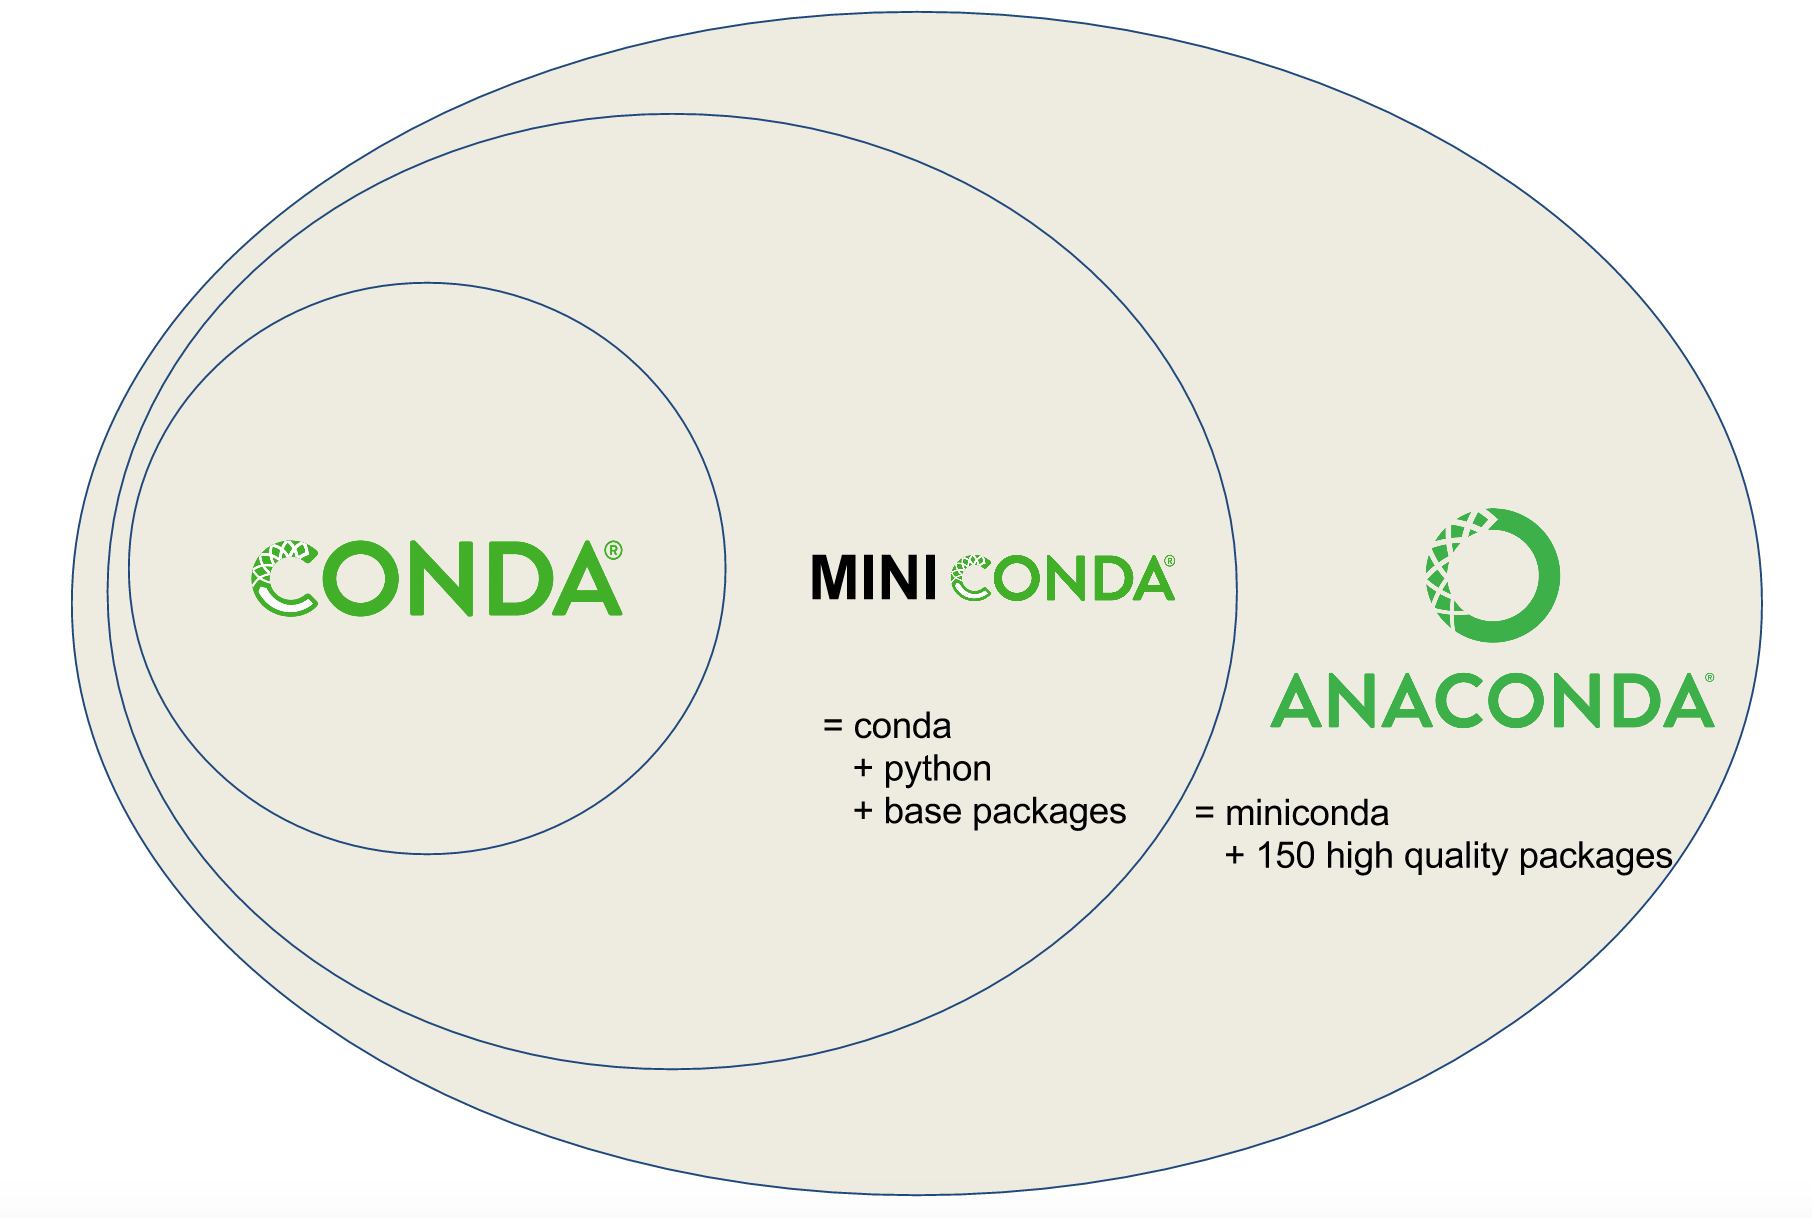
\includegraphics[width=\textwidth]{graphics/conda_mini_ana.png}
    \caption{Relationship between \conda, \texttt{miniconda}, and \texttt{anaconda}.}
    \label{fig:conda_mini_ana}
\end{marginfigure}

\section{Downloading}

\section{Installation}

\subsection{Testing}

\subsection{Updating}

\subsection{Common problems}

\section{Installing libraries}
like \texttt{numpy}, \texttt{matplotlib}, \texttt{pandas}, \texttt{scikit-learn}, and \texttt{networkx}

\section{Maintaining libraries}

\section{Removing libraries}

\section{Environments}
% LaTeX Canvas: Chapter Outline
\chapter{Jupyter}
\label{ch:jupyter}

\section*{Purpose}
Jupyter notebooks are an effective medium for exploratory analysis because they combine code, results, and narrative. The same flexibility can also create confusion: wrong working directories, out-of-order execution, hidden state, and notebooks that cannot be reproduced. This chapter teaches novices how to launch Jupyter correctly, navigate files, use cells effectively, run shell commands safely, and adopt notebook discipline so work remains interpretable and reproducible.

\section*{Learning objectives}
By the end of this chapter, you should be able to:
\begin{enumerate}
\item Launch Jupyter Notebook or JupyterLab from the command line in the correct folder.
\item Diagnose the common ``Jupyter has no files'' problem (wrong working directory).
\item Explain kernels, sessions, and the difference between Notebook and JupyterLab.
\item Use cell types (code/markdown/raw), move cells, and manage execution order.
\item Use IPython magics and run shell commands inside a notebook safely.
\item Structure a notebook for readability: headings, narrative, and controlled outputs.
\item Make notebooks reproducible: restart-and-run-all, environment capture, and data provenance.
\item Convert notebooks into scripts/reports when appropriate.
\end{enumerate}

\section*{Running theme: notebooks are documents \emph{and} programs}
A notebook should read like a report and execute like a program. The discipline is to ensure both.

\section{Mental models: what Jupyter is doing}
\subsection{Notebook vs JupyterLab}
\begin{itemize}
\item \textbf{Jupyter Notebook} (classic) is a single-document interface.
\item \textbf{JupyterLab} is a multi-document environment (files, terminals, notebooks, consoles).
\item Both run on the same concepts: a server, a browser UI, and kernels.
\end{itemize}

\subsection{Server, browser, kernel}
\begin{itemize}
\item \textbf{Server:} the process you start (the thing listening on \texttt{localhost:8888}).
\item \textbf{Browser UI:} where you edit and run cells.
\item \textbf{Kernel:} the language runtime executing your code (Python, R, etc.).
\end{itemize}

\subsection{State and order}
\begin{itemize}
\item Notebooks allow executing cells out of order.
\item The kernel remembers variables from prior cells.
\item ``It works on my notebook'' often means hidden state.
\end{itemize}

\section{Launching Jupyter the right way}
\subsection{The rule: start from your project folder}
\begin{itemize}
\item Open a terminal.
\item \textbf{Navigate} to the folder containing your notebooks (your project root).
\item Start Jupyter there.
\end{itemize}

\subsection{Launch commands (conceptual)}
\begin{itemize}
\item \texttt{jupyter lab}
\item \texttt{jupyter notebook}
\item Common pattern: pass a directory path if you are not already in it.
\end{itemize}

\subsection{Verifying you launched in the correct directory}
\begin{itemize}
\item In the terminal: confirm the current directory before launching.
\item In the UI: confirm the file browser shows your expected folder tree.
\item Create a small marker file (e.g., \texttt{PROJECT\_ROOT.txt}) so you can tell when you are in the right place.
\end{itemize}

\subsection{Launching from an environment (important for students)}
\begin{itemize}
\item Ensure you started the correct environment (conda/venv) before launching Jupyter.
\item Know how to confirm which Python/kernel is in use (kernel name, version cell).
\end{itemize}

\section{The common failure: ``Jupyter shows no notebooks''}
\subsection{Symptom}
\begin{itemize}
\item The Jupyter file browser is empty or shows a different folder than expected.
\item Your notebook cannot find \texttt{data/} even though it exists.
\end{itemize}

\subsection{Root cause: wrong working directory / wrong server}
\begin{itemize}
\item You launched Jupyter from a different folder.
\item You have multiple Jupyter servers running and you opened the wrong tab.
\item You launched from the wrong environment, so kernels and paths differ.
\end{itemize}

\subsection{Fix checklist}
\begin{enumerate}
\item Stop Jupyter (Ctrl+C in the terminal) and close the browser tab.
\item In the terminal: \textbf{navigate} to the correct folder.
\item Relaunch Jupyter.
\item If still wrong: check for other running Jupyter servers and shut them down.
\item Add a first cell in notebooks that prints the working directory.
\end{enumerate}

\section{Notebook mechanics: cells and execution}
\subsection{Cell types}
\begin{description}
\item[Code] Executes in the kernel.
\item[Markdown] Narrative text, headings, equations, images.
\item[Raw] Passed through without formatting (rare; use intentionally).
\end{description}

\subsection{Running cells}
\begin{itemize}
\item Run one cell vs run all.
\item Interrupt vs restart kernel.
\item Understand the execution count as evidence of order.
\end{itemize}

\subsection{Moving and organizing cells}
\begin{itemize}
\item Move cells to keep the story and the computation aligned.
\item Use headings to create a navigable outline.
\item Keep imports and configuration near the top.
\end{itemize}

\subsection{Output management}
\begin{itemize}
\item Avoid printing entire datasets.
\item Prefer summaries (shape, head, descriptive stats).
\item Clear and re-run outputs as part of reproducibility checks.
\end{itemize}

\section{Running shell commands inside notebooks (responsibly)}
\subsection{Why this is useful}
\begin{itemize}
\item Quick checks: list files, inspect paths, verify data presence.
\item Lightweight automation: download a file, decompress, run a command-line tool.
\end{itemize}

\subsection{Two mechanisms: ``bang'' and magics}
\begin{itemize}
\item \textbf{Bang commands} (\texttt{!}): run a shell command from a code cell.
\item \textbf{Magics} (\texttt{%} and \texttt{%%}): special IPython commands for workflows.
\end{itemize}

\subsection{Common magics for students}
\begin{itemize}
\item Directory awareness: \texttt{%pwd}, \texttt{%cd}
\item Timing: \texttt{%time}, \texttt{%timeit}
\item Multi-line shell blocks (when taught): \texttt{%%bash} (or equivalent)
\end{itemize}

\subsection{Safety rules for shell commands in notebooks}
\begin{itemize}
\item Treat shell commands as potentially destructive.
\item Avoid \texttt{sudo} from notebooks.
\item Never embed secrets (tokens, passwords) in notebook cells.
\item Record what the command does and why (markdown cell above).
\item Prefer reproducible commands over manual clicking.
\end{itemize}

\section{Notebook style and discipline (how to write a notebook that survives)}
\subsection{Structure: a notebook template}
\begin{itemize}
\item Title + one-paragraph purpose.
\item Setup: imports, configuration, paths.
\item Data acquisition and provenance.
\item Cleaning and validation checks.
\item Analysis/modeling.
\item Results and interpretation.
\item Next steps / limitations.
\end{itemize}

\subsection{Narrative: make the notebook readable}
\begin{itemize}
\item Use markdown headings and short explanatory paragraphs.
\item Explain assumptions and decisions (why this filter? why this join?).
\item Use captions on plots and tables.
\end{itemize}

\subsection{Reproducibility discipline}
\begin{itemize}
\item Use a consistent top-to-bottom execution order.
\item Periodically: \textbf{Restart kernel and Run All}.
\item Avoid hidden dependencies on prior interactive state.
\item Prefer functions over repeated copy/paste code.
\item Prefer relative paths inside a project.
\end{itemize}

\subsection{Environment capture (student level)}
\begin{itemize}
\item Record: Python version, key package versions, and OS.
\item Store environment files (e.g., \texttt{environment.yml}) when using conda.
\item Keep datasets and generated artifacts in well-labeled folders.
\end{itemize}

\subsection{Outputs and size control}
\begin{itemize}
\item Large outputs make notebooks slow and hard to version.
\item Avoid embedding huge binary blobs.
\item Prefer saving outputs to files (\texttt{data/processed}, \texttt{figures/}).
\end{itemize}

\section{Notebook pitfalls and how to prevent them}
\subsection{Out-of-order execution}
\begin{itemize}
\item Prevention: restart-and-run-all checks.
\item Signal: execution counts jump around; variables appear ``from nowhere.''
\end{itemize}

\subsection{Wrong kernel / wrong environment}
\begin{itemize}
\item Symptom: imports fail or versions differ from expectations.
\item Prevention: name kernels clearly; confirm versions in a top cell.
\end{itemize}

\subsection{File not found (paths)}
\begin{itemize}
\item Symptom: \texttt{FileNotFoundError} despite file existing.
\item Prevention: print working directory; use project-relative paths.
\end{itemize}

\subsection{Long-running or stuck cells}
\begin{itemize}
\item Learn: interrupt vs restart.
\item Add progress indicators or timing.
\item Move expensive work to scripts or batch runs when appropriate.
\end{itemize}

\section{When to move from notebooks to scripts (and back)}
Chapter~\ref{ch:scripts-vs-notebooks} covers the scripting workflow in full; this section explains how notebooks and scripts fit together.
\subsection{Notebook strengths}
\begin{itemize}
\item Exploration, explanation, and sharing results.
\end{itemize}

\subsection{Script strengths}
\begin{itemize}
\item Production runs, automation, CI testing, and parameterized workflows.
\end{itemize}

\subsection{A practical boundary for students}
\begin{itemize}
\item Keep exploration in notebooks.
\item Extract stable logic into \texttt{src/} as functions.
\item Keep the notebook as a narrative driver calling those functions.
\end{itemize}

\section{Worked examples (outline)}
\subsection{Example 1: Launch Jupyter in the right place}
\begin{itemize}
\item Navigate to a project folder.
\item Start JupyterLab.
\item Create a notebook and verify the working directory.
\end{itemize}

\subsection{Example 2: Debug ``no files'' / wrong directory}
\begin{itemize}
\item Demonstrate launching from the wrong folder.
\item Diagnose and fix by relaunching from the correct path.
\item Add a working-directory check cell.
\end{itemize}

\subsection{Example 3: Shell commands for file checks}
\begin{itemize}
\item List project files.
\item Confirm a dataset exists and report size.
\item Use \texttt{%pwd} and \texttt{%cd} intentionally.
\end{itemize}

\subsection{Example 4: Make a notebook reproducible}
\begin{itemize}
\item Add headings and narrative.
\item Extract repeated code into functions.
\item Restart kernel and run all; fix hidden-state bugs.
\end{itemize}

\section{Templates}
\subsection{Template A: Notebook header block}
\begin{verbatim}
Title:
Author:
Date:
Purpose:
Data sources:
Environment:

* Python:
* Key packages:
  How to run:
* Restart kernel and Run All
  Outputs:
* Where figures/tables are saved
  \end{verbatim}

\subsection{Template B: Reproducibility checklist cell}
\begin{verbatim}

# Reproducibility check

# 1) print working directory

# 2) print python and package versions

# 3) confirm data files exist

# 4) run a small smoke test

\end{verbatim}

\section{Exercises}
\begin{enumerate}
\item Launch JupyterLab from a project directory and create a notebook that prints its working directory.
\item Intentionally launch from the wrong directory; diagnose and fix.
\item Practice cell operations: convert code to markdown, move cells, and create headings.
\item Use one shell command (via \texttt{!}) to list files and one magic (\texttt{%pwd}) to confirm location.
\item Take a messy notebook and refactor it into sections with narrative and a restart-and-run-all proof.
\item Extract one repeated block into a function and verify outputs are unchanged.
\end{enumerate}

\section{One-page checklist}
\begin{itemize}
\item I launch Jupyter from the correct project folder (or pass the correct directory).
\item I can diagnose ``no files'' as a working-directory/server mix-up.
\item I understand kernels and can choose the correct one.
\item I use markdown headings to structure the notebook.
\item I keep a top-to-bottom execution order and periodically restart-and-run-all.
\item I use shell commands and magics sparingly, with explanations and no secrets.
\item I record environment details and keep data provenance explicit.
\item I keep outputs controlled and store large artifacts outside the notebook.
\end{itemize}

% \appendix
\section{Quick reference: common launch and debugging moves}
\begin{itemize}
\item Confirm working directory before launching.
\item If you see the wrong files: stop server, relaunch in correct directory.
\item If imports fail: check kernel/environment.
\item If execution hangs: interrupt; then restart if needed.
\end{itemize}

\section{Quick reference: IPython conveniences}
\begin{itemize}
\item \texttt{!command} runs a shell command.
\item \texttt{%pwd} shows current directory; \texttt{%cd} changes it.
\item Use timing magics to understand slow cells.
\end{itemize}

% LaTeX Canvas: Chapter Outline
\chapter{Scripting}
\label{ch:scripts-vs-notebooks}

\section*{Purpose}
As students progress, the limiting factor is rarely ``can you write code''; it is whether your work can be reused, rerun, and explained. Scripts complement notebooks by making work \emph{repeatable} from the command line and easier to automate, test, and share. This chapter teaches how to write simple scripts, import your own code into notebooks, translate notebooks into scripts, pass parameters from the command line, and make deliberate notebook-versus-script choices.

\section*{Learning objectives}
By the end of this chapter, a reader should be able to:
\begin{enumerate}
\item Write a Python script that can be run from the command line and imported as a module.
\item Organize reusable code into functions and (optionally) a small \texttt{src/} module.
\item Import custom scripts into a Jupyter notebook and reload changes during iteration.
\item Convert notebooks to scripts (and scripts to notebooks) using standard tools.
\item Pass parameters into scripts using a command-line interface (CLI) pattern.
\item Explain trade-offs: when a notebook is the right tool and when a script is.
\item Use a ``notebook as narrative, script as engine'' pattern to keep work reproducible.
\end{enumerate}

\section*{Running theme: separate \emph{logic} from \emph{presentation}}
The logic (data loading, cleaning, analysis) should live in importable functions. The notebook (or script) should orchestrate and explain.

\section{Mental models and vocabulary}
\subsection{Script, module, package}
\begin{description}
\item[Script] A file you run (e.g., \texttt{python analyze.py}).
\item[Module] A file you import (e.g., \texttt{import analysis}).
\item[Package] A directory of modules (typically with \texttt{\_\_init\_\_.py}) installed or importable.
\end{description}

\subsection{Entry point vs library code}
\begin{itemize}
\item \textbf{Entry point:} parsing parameters, calling functions, writing outputs.
\item \textbf{Library code:} reusable functions/classes that do the work.
\end{itemize}

\subsection{Working directory and paths}
\begin{itemize}
\item Scripts and notebooks depend on the working directory for relative paths.
\item Habit: define a project root and use consistent relative paths inside it.
\end{itemize}

\section{Writing scripts: the essentials}
\subsection{A minimal script structure}
\begin{itemize}
\item Imports
\item Constants/config
\item Functions
\item \texttt{main()} function
\item \texttt{if \_\_name\_\_ == "\_\_main\_\_":} block
\end{itemize}

\subsection{Why \texttt{main()} matters}
\begin{itemize}
\item Enables clean separation between code that runs on import vs code that runs on execution.
\item Makes the file usable both as a script and as an importable module.
\end{itemize}

\subsection{Inputs, outputs, and side effects}
\begin{itemize}
\item Inputs: file paths, URLs, parameters.
\item Outputs: files (CSV, figures), printed summaries, logs.
\item Prefer writing outputs to named folders (e.g., \texttt{data/processed}, \texttt{figures/}).
\end{itemize}

\subsection{Print vs logging (intro level)}
\begin{itemize}
\item Use print for small, human-facing status.
\item Introduce logging as a structured alternative for larger scripts.
\end{itemize}

\section{Organizing reusable code: from one file to \texttt{src/}}
\subsection{From monolith to functions}
\begin{itemize}
\item Identify repeated blocks and extract them into functions.
\item Make functions pure when possible: inputs in, outputs out.
\end{itemize}

\subsection{A simple project layout}
\begin{itemize}
\item \texttt{notebooks/} (narrative and exploration)
\item \texttt{src/} (reusable code)
\item \texttt{scripts/} (CLI entry points)
\item \texttt{data/raw}, \texttt{data/processed}, \texttt{figures/}
\item \texttt{README.md} (how to run)
\end{itemize}

\subsection{Import paths without pain (student-safe guidance)}
\begin{itemize}
\item Prefer running from the project root so imports and relative paths behave.
\item Avoid copying code between notebooks; import instead.
\item If imports are confusing, treat it as a project-structure problem, not a ``magic command'' problem.
\end{itemize}

\section{Loading custom scripts into notebooks}
\subsection{The basic pattern: import your code}
\begin{itemize}
\item Place reusable functions in \texttt{src/} (or a clearly named module file).
\item Import them in the notebook and call them like normal functions.
\item Keep notebooks thin: analysis orchestration + narrative.
\end{itemize}

\subsection{Iterating on imported code: reloading}
\begin{itemize}
\item Notebooks keep a long-lived kernel; imports do not automatically update.
\item Teach a safe workflow:
\begin{enumerate}
\item Edit code in the editor.
\item Reload the module (conceptual introduction to \texttt{importlib.reload}).
\item Re-run a small test cell.
\end{enumerate}
\end{itemize}

\subsection{Alternative: run a script from a notebook}
\begin{itemize}
\item Use notebook mechanisms to execute a script when appropriate.
\item Warn: running external processes can create confusing state splits (kernel state vs process state).
\end{itemize}

\subsection{Notebook ``smoke test'' cell}
\begin{itemize}
\item A small cell near the top that:
\begin{itemize}
\item prints working directory
\item checks required files exist
\item imports your \texttt{src/} modules
\item prints key versions
\end{itemize}
\end{itemize}

\section{Passing parameters from the command line}
\subsection{Why parameterize scripts}
\begin{itemize}
\item Make the same analysis run on different datasets or time ranges.
\item Enable automation (scheduled runs, batch processing).
\item Reduce copy/paste ``variant'' scripts.
\end{itemize}

\subsection{Three levels of parameterization}
\begin{description}
\item[Level 1: constants] edit values in the script (fast, not scalable).
\item[Level 2: config files] store parameters in a small text file (scalable for teams).
\item[Level 3: CLI arguments] pass parameters at run time (best for automation).
\end{description}

\subsection{The CLI pattern (student baseline)}
\begin{itemize}
\item Define required positional arguments (e.g., input file).
\item Define optional flags (e.g., \texttt{--out}, \texttt{--seed}, \texttt{--limit}).
\item Provide clear help text and defaults.
\end{itemize}

\subsection{Validating inputs}
\begin{itemize}
\item Check that input paths exist.
\item Validate parameter ranges (e.g., nonnegative integers).
\item Fail fast with helpful error messages.
\end{itemize}

\subsection{Reproducibility and auditability}
\begin{itemize}
\item Print or log the resolved parameters at start.
\item Write outputs to a deterministic location based on parameters.
\item Record the command used to run the script in \texttt{README.md} or an output metadata file.
\end{itemize}

\section{Translating notebooks into scripts (and vice versa)}
\subsection{Why convert}
\begin{itemize}
\item Scripts are easier to run in batch jobs and automation.
\item Scripts produce cleaner diffs in version control.
\item Converting can help reveal hidden-state problems.
\end{itemize}

\subsection{One-way conversion: notebook to script}
\begin{itemize}
\item Convert an \texttt{.ipynb} into a \texttt{.py} for review, reuse, or batch runs.
\item Treat the output as a starting point: refactor into functions.
\end{itemize}

\subsection{Round-trip conversion: paired notebooks}
\begin{itemize}
\item Pair an \texttt{.ipynb} with a text representation (e.g., percent script) so you can edit in a normal editor.
\item Benefit: better diffs, easier merges.
\end{itemize}

\subsection{Parameterizing notebooks (bridge to automation)}
\begin{itemize}
\item Some workflows keep notebooks but run them repeatedly with different parameters.
\item Introduce the concept of tagging a ``parameters'' cell and executing programmatically.
\end{itemize}

\section{Notebook versus script: trade-offs and decision rules}
\subsection{Notebooks are best for}
\begin{itemize}
\item Exploration and rapid iteration.
\item Teaching, explanation, and narrative analysis.
\item Sharing a computational story with plots and commentary.
\end{itemize}

\subsection{Scripts are best for}
\begin{itemize}
\item Repeatable runs with parameters.
\item Automation (cron, schedulers, CI).
\item Long-running jobs and robust logging.
\item Clean version control diffs and code review.
\end{itemize}

\subsection{Common hybrid pattern (recommended)}
\begin{itemize}
\item \textbf{Notebook:} narrative driver, figures, interpretation.
\item \textbf{src/:} reusable functions.
\item \textbf{scripts/:} CLI entry points for batch runs.
\end{itemize}

\subsection{Smells that suggest ``move to a script''}
\begin{itemize}
\item You manually rerun the same notebook with small changes.
\item The notebook takes a long time and you want it to run unattended.
\item You need command-line parameters or scheduled runs.
\item You need robust logs, retries, or consistent outputs.
\end{itemize}

\subsection{Smells that suggest ``stay in a notebook''}
\begin{itemize}
\item The primary goal is interpretation and communication.
\item The analysis is exploratory and changing quickly.
\item You are teaching or documenting reasoning.
\end{itemize}

\section{Best practices: making scripts and notebooks play well together}
\subsection{Make data and paths explicit}
\begin{itemize}
\item Avoid absolute paths.
\item Use a consistent project root.
\item Add a small path-check function used by both notebooks and scripts.
\end{itemize}

\subsection{Minimize hidden state}
\begin{itemize}
\item In notebooks: restart-and-run-all checks.
\item In scripts: pure functions and explicit parameters.
\end{itemize}

\subsection{Document how to run}
\begin{itemize}
\item A \texttt{README.md} with one ``copy/paste to run'' command.
\item Record expected inputs, outputs, and runtime.
\end{itemize}

\subsection{Version control discipline}
\begin{itemize}
\item Keep notebooks tidy: clear noisy outputs; avoid huge embedded data.
\item Prefer paired notebook formats or conversion to scripts for review.
\end{itemize}

\section{Worked examples (outline)}
\subsection{Example 1: Turn notebook code into importable functions}
\begin{itemize}
\item Identify a repeated transform.
\item Extract into \texttt{src/cleaning.py}.
\item Import and call from the notebook.
\end{itemize}

\subsection{Example 2: Write a CLI script around your functions}
\begin{itemize}
\item Create \texttt{scripts/run\_cleaning.py}.
\item Parse \texttt{--input} and \texttt{--output}.
\item Write outputs and print a short run summary.
\end{itemize}

\subsection{Example 3: Debug ``it imports in the terminal but not in the notebook''}
\begin{itemize}
\item Diagnose kernel/environment mismatch.
\item Diagnose project root/working directory mismatch.
\item Fix by selecting the correct kernel and running from the project root.
\end{itemize}

\subsection{Example 4: Convert a notebook to a script and refactor}
\begin{itemize}
\item Convert \texttt{analysis.ipynb} to \texttt{analysis.py}.
\item Clean the result: remove interactive-only cells, extract functions.
\item Add a minimal \texttt{main()} and CLI args.
\end{itemize}

\subsection{Example 5: Parameterize a notebook for repeated execution (optional)}
\begin{itemize}
\item Add a parameters cell.
\item Execute with different parameter sets and save outputs.
\end{itemize}

\section{Templates}
\subsection{Template A: Minimal script skeleton}
\begin{verbatim}
"""One-sentence purpose.

Inputs:
Outputs:
How to run:
"""

from pathlib import Path

def main(...):
...

if **name** == "**main**":
main(...)
\end{verbatim}

\subsection{Template B: Minimal CLI skeleton (conceptual)}
\begin{verbatim}
import argparse

def parse_args():
p = argparse.ArgumentParser(...)
p.add_argument("--input", required=True)
p.add_argument("--output", required=True)
return p.parse_args()

def main():
args = parse_args()
...

if **name** == "**main**":
main()
\end{verbatim}

\subsection{Template C: Notebook that calls scriptable functions}
\begin{verbatim}

# 1) Purpose + imports

# 2) Parameters (as variables)

# 3) Call functions from src/

# 4) Save outputs

# 5) Interpretation

# 6) Restart-and-run-all proof

\end{verbatim}

\section{Exercises}
\begin{enumerate}
\item Write a script that loads a CSV and prints a short summary (rows, columns, missingness).
\item Refactor the script so the summary logic is in a function and the script is only an entry point.
\item Import that function into a notebook and use it on two datasets.
\item Add a CLI with \texttt{--input} and \texttt{--output} flags.
\item Convert a notebook to a script and identify at least three hidden-state problems you had to fix.
\item Write a short paragraph explaining whether your project should be a notebook, a script, or a hybrid---and why.
\end{enumerate}

\section{One-page checklist}
\begin{itemize}
\item My script has a \texttt{main()} and does not run heavy work on import.
\item Reusable logic lives in importable functions/modules.
\item I can import my own code into notebooks and reload changes when iterating.
\item I can run the same analysis via a CLI with parameters.
\item I know how to convert notebooks to scripts and use conversion to improve reproducibility.
\item I choose notebooks for narrative/exploration and scripts for repeatable/automated runs.
\end{itemize}

\appendix
\section{Quick reference: common tools (conceptual)}
\begin{itemize}
\item Notebook conversion to scripts and reports.
\item Paired notebook formats for better diffs.
\item Parameterized execution of notebooks for batch runs.
\end{itemize}

\part{Project Management}
% LaTeX Canvas: Chapter Outline
\chapter{Project Management}
\label{ch:project-management}

\section*{Purpose}
Most student projects fail for non-technical reasons: files scattered across desktops, unclear goals, missing data provenance, undocumented assumptions, and work tracked in private messages rather than a shared system. This chapter introduces lightweight project management practices that make small data-science projects stable, auditable, and collaborative.

\section*{Learning objectives}
By the end of this chapter, you should be able to:
\begin{enumerate}
\item Define a project goal, success criteria, and constraints in a short project brief.
\item Set up a reproducible project structure with clear locations for data, code, notebooks, outputs, and docs.
\item Apply data management hygiene: provenance, naming, immutability of raw data, and data dictionaries.
\item Write minimal project documentation that enables another person (or future you) to reproduce results.
\item Use issue tracking to plan work, document decisions, and coordinate collaboration.
\item Maintain a simple cadence for planning, execution, review, and delivery.
\end{enumerate}

\section*{Running theme: make progress visible and work repeatable}
A well-managed project makes its assumptions and status legible: what the data are, what changed, what remains, and how to rerun.

\section{Mental model: a project is a system of artifacts}
\subsection{Artifacts you must manage}
\begin{itemize}
\item \textbf{Data:} raw inputs, processed outputs, intermediate files.
\item \textbf{Code:} scripts, reusable modules, notebooks.
\item \textbf{Environment:} dependencies and runtime assumptions.
\item \textbf{Documentation:} purpose, decisions, usage, and interpretation.
\item \textbf{Work tracking:} tasks, bugs, questions, and priorities.
\end{itemize}

\subsection{The lifecycle: plan $\rightarrow$ build $\rightarrow$ verify $\rightarrow$ deliver}
\begin{itemize}
\item \textbf{Plan:} decide what success looks like.
\item \textbf{Build:} implement data pipelines/analysis.
\item \textbf{Verify:} check quality, reproduce outputs.
\item \textbf{Deliver:} package results and communicate limitations.
\end{itemize}

\section{Project planning for novices (lightweight, not bureaucratic)}
\subsection{The one-page project brief}
\begin{itemize}
\item Problem statement (one paragraph).
\item Audience and use case.
\item Deliverables (tables, plots, memo, dashboard, model).
\item Success criteria (what ``done'' means).
\item Constraints (time, compute, access, privacy).
\item Risks and unknowns (data availability, definitions, biases).
\end{itemize}

\subsection{Decompose work into milestones}
\begin{itemize}
\item Milestone 1: data acquisition + intake note.
\item Milestone 2: cleaning + data dictionary.
\item Milestone 3: analysis + validation.
\item Milestone 4: outputs + narrative + reproducibility check.
\end{itemize}

\subsection{Define decision points}
\begin{itemize}
\item What choices might change results? (filters, joins, missingness handling)
\item Where will you record those decisions? (issues, changelog, notebook narrative)
\end{itemize}

\section{Reproducible project structure}
\subsection{Design principles}
\begin{itemize}
\item One project folder = one project.
\item Raw data are read-only.
\item Outputs are reproducible from code.
\item Paths are relative to the project root.
\item Clear separation: data vs code vs docs vs outputs.
\end{itemize}

\subsection{A student-friendly directory template}
\begin{verbatim}
project/
README.md
environment.yml   (or requirements.txt)
data/
raw/
processed/
external/
notebooks/
src/
scripts/
reports/
figures/
docs/
tests/            (optional)
\end{verbatim}

\subsection{Naming conventions and consistency}
\begin{itemize}
\item Use lowercase and hyphens/underscores (choose one).
\item Date stamps for snapshots (e.g., \texttt{2026-01-08}).
\item Avoid spaces and ambiguous names (\texttt{final\_final2.csv}).
\end{itemize}

\subsection{What goes where (and what does not)}
\begin{itemize}
\item \texttt{data/raw}: original sources; never edited.
\item \texttt{data/processed}: generated outputs from cleaning.
\item \texttt{notebooks}: narrative drivers; keep tidy.
\item \texttt{src}: reusable functions and modules.
\item \texttt{scripts}: command-line entry points.
\item \texttt{reports/figures}: final artifacts for sharing.
\item Avoid storing secrets or credentials anywhere in the repo.
\end{itemize}

\section{Data management hygiene}
\subsection{Provenance: where did this data come from?}
\begin{itemize}
\item Source URL or file origin.
\item Retrieval date/time.
\item License/terms of use.
\item Any access restrictions or privacy considerations.
\end{itemize}

\subsection{Raw data immutability}
\begin{itemize}
\item Treat raw data as evidence: do not edit.
\item If you must fix an obvious error, do it in a processing step that is documented.
\end{itemize}

\subsection{Data dictionary and codebook}
\begin{itemize}
\item One table with: variable name, type, meaning, units, allowable values, missingness codes.
\item Record transformations: derived fields, recodes, joins.
\end{itemize}

\subsection{Versioning data}
\begin{itemize}
\item When datasets change, create dated snapshots or version tags.
\item Record checksums or file sizes for integrity (intro concept).
\item Keep ``what changed'' notes (new rows, new columns, schema shifts).
\end{itemize}

\subsection{Sensitive data hygiene (baseline)}
\begin{itemize}
\item Identify whether data contain identifiers.
\item Minimize access: store sensitive data outside repos when required.
\item Never commit secrets, API keys, or tokens.
\item Redact or aggregate before sharing.
\end{itemize}

\section{Documentation that makes a project runnable}
Chapter~\ref{ch:documentation} covers how to find, read, and write technical documentation in depth; this section focuses on the documentation artifacts specific to a project.
\subsection{README as the single source of truth}
\begin{itemize}
\item What the project does (one paragraph).
\item What data are required and where they go.
\item How to set up the environment.
\item One ``copy/paste'' command to reproduce core outputs.
\item How to interpret outputs (where to find the key tables/figures).
\end{itemize}

\subsection{Decision log}
\begin{itemize}
\item Record consequential choices: filtering rules, outlier handling, join keys.
\item Store decisions in issues or a dedicated \texttt{DECISIONS.md}.
\end{itemize}

\subsection{Docstrings and inline comments (just enough)}
\begin{itemize}
\item Explain intent, not obvious syntax.
\item Document inputs, outputs, assumptions.
\end{itemize}

\subsection{Reproducibility notes}
\begin{itemize}
\item Environment file is required.
\item Note OS-specific dependencies.
\item Include a small ``smoke test'' script or notebook cell.
\end{itemize}

\section{Issue tracking fundamentals (for students)}
\subsection{Why issues are not just for bugs}
\begin{itemize}
\item Tasks, questions, data problems, and design decisions.
\item A shared memory and audit trail.
\end{itemize}

\subsection{Anatomy of a good issue}
\begin{itemize}
\item Clear title: action + object.
\item Description: context, objective, definition of done.
\item Evidence: links, screenshots, error messages.
\item Labels: type (bug/task/question), priority, area (data/code/docs).
\end{itemize}

\subsection{Issue workflow: triage $\rightarrow$ do $\rightarrow$ review $\rightarrow$ close}
\begin{itemize}
\item Triage: clarify, label, assign, and break down.
\item Do: create a branch or working copy tied to the issue (concept).
\item Review: verify outputs, update docs.
\item Close: summarize what changed and link artifacts.
\end{itemize}

\subsection{Milestones and project boards (optional)}
\begin{itemize}
\item Milestones map to deliverables.
\item Boards visualize status (To do / Doing / Done).
\item Keep it lightweight: avoid over-customization early.
\end{itemize}

\section{Quality gates: make ``done'' meaningful}
\subsection{The reproducibility check}
\begin{itemize}
\item Fresh environment or clean restart.
\item Run the pipeline end-to-end.
\item Confirm outputs match expectations.
\end{itemize}

\subsection{Data checks}
\begin{itemize}
\item Row/column counts.
\item Missingness summary.
\item Value ranges and plausibility.
\item Join coverage and key uniqueness.
\end{itemize}

\subsection{Output checks}
\begin{itemize}
\item Figures labeled, units clear, captions present.
\item Tables have consistent formatting and definitions.
\item Narrative explains limitations and uncertainty.
\end{itemize}

\section{Common failure modes and how to prevent them}
\subsection{Folder chaos and lost files}
\begin{itemize}
\item Prevention: stable project root + fixed structure.
\item Recovery: search by extension/date; reconstruct from outputs.
\end{itemize}

\subsection{Silent data drift}
\begin{itemize}
\item Prevention: snapshot raw data; record retrieval dates and checksums.
\item Detection: schema checks and summary stats comparisons.
\end{itemize}

\subsection{Undocumented assumptions}
\begin{itemize}
\item Prevention: decision log + notebook narrative.
\item Practice: ``if this changed, results would change'' gets documented.
\end{itemize}

\subsection{Work tracked in private channels}
\begin{itemize}
\item Prevention: issues for tasks/questions; link decisions and artifacts.
\end{itemize}

\section{Worked examples (outline)}
\subsection{Example 1: Start a new course project in 20 minutes}
\begin{itemize}
\item Create the folder structure.
\item Add environment file.
\item Write a README with ``how to run''.
\end{itemize}

\subsection{Example 2: Intake a dataset with provenance and a data dictionary}
\begin{itemize}
\item Place raw file.
\item Write provenance notes.
\item Draft codebook and a first-pass quality report.
\end{itemize}

\subsection{Example 3: Use issues to manage a cleaning pipeline}
\begin{itemize}
\item Create issues for missingness, type conversions, duplicates, joins.
\item Close each issue with a summary and link to outputs.
\end{itemize}

\subsection{Example 4: Final reproducibility check before submission}
\begin{itemize}
\item Recreate env.
\item Run end-to-end.
\item Confirm outputs and update README.
\end{itemize}

\section{Templates}
\subsection{Template A: One-page project brief}
\begin{verbatim}
Title:
Problem:
Audience:
Deliverables:
Success criteria:
Constraints:
Risks/unknowns:
Milestones:
\end{verbatim}

\subsection{Template B: README skeleton}
\begin{verbatim}

# Project name

## Purpose

## Data

* Source:
* Retrieved:
* License/notes:
* Location: data/raw/

## Setup

* Create environment:
* Activate environment:

## Run

* Command(s) to reproduce key outputs:

## Outputs

* reports/
* figures/

## Notes

* Decisions and limitations
  \end{verbatim}

\subsection{Template C: Issue template (student version)}
\begin{verbatim}
Title:
Type: bug/task/question
Context:
What I tried:
Evidence (errors, screenshots, links):
Definition of done:
\end{verbatim}

\section{Exercises}
\begin{enumerate}
\item Create a new project folder using the template and write a README that someone else could follow.
\item Intake a dataset: place it in \texttt{data/raw}, write provenance notes, and draft a data dictionary.
\item Create five issues that decompose the project into milestones and tasks; label and prioritize them.
\item Implement one task and close its issue with a short ``what changed'' summary.
\item Perform a reproducibility check by recreating your environment and rerunning the pipeline.
\end{enumerate}

\section{One-page checklist}
\begin{itemize}
\item I have a clear project goal and definition of done.
\item My project folder has a reproducible structure.
\item Raw data are immutable and provenance is recorded.
\item I maintain a data dictionary and transformation notes.
\item My README explains setup, run, and outputs.
\item Work is tracked in issues with labels and clear closure notes.
\item I can reproduce results from a clean environment.
\end{itemize}

% \appendix
\section{Quick reference: ``minimum viable'' project operations}
\begin{itemize}
\item Create structure.
\item Write README.
\item Record environment.
\item Intake data with provenance.
\item Track work in issues.
\item Reproduce end-to-end before delivery.
\end{itemize}

% LaTeX Canvas: Chapter Outline
\chapter{Version Control}
\label{ch:git-github}

\section*{Purpose}
Version control is the safety system for technical work. Git records a history of changes so you can recover, compare, and collaborate without overwriting each other. GitHub adds shared hosting, review workflows, and discussion tools. This chapter teaches novice-friendly Git fundamentals and the everyday GitHub workflows students need: pushing and pulling, branches and merges, pull requests, forks, and review/commenting practices.

\section*{Learning objectives}
By the end of this chapter, a reader should be able to:
\begin{enumerate}
\item Explain what version control is and why Git is ``distributed.''
\item Create or clone a repository and make clean commits.
\item Understand the working tree, staging area, and commit history.
\item Use branches for features/fixes and merge changes safely.
\item Work with remotes (\texttt{origin}, \texttt{upstream}) and synchronize using fetch/pull/push.
\item Use GitHub to open a pull request, respond to feedback, and merge.
\item Resolve common merge conflicts with a disciplined playbook.
\item Use forks for contributing to projects you do not control.
\item Write good commit messages and PR descriptions; comment constructively in reviews.
\end{enumerate}

\section*{Running theme: make changes small, reviewable, and reversible}
A healthy Git workflow favors small commits, small pull requests, clear messages, and frequent synchronization.

\section{Mental models and vocabulary}
\subsection{Repository, snapshot, history}
\begin{itemize}
\item A \textbf{repository} is your project folder plus a hidden \texttt{.git} directory.
\item A \textbf{commit} is a snapshot of tracked files with metadata (author, time, message).
\item Git history is a graph, not a single line.
\end{itemize}

\subsection{The three zones: working tree, staging area, commits}
\begin{itemize}
\item \textbf{Working tree:} your edited files.
\item \textbf{Staging area (index):} the exact changes you plan to commit.
\item \textbf{Commit:} saved snapshot in history.
\end{itemize}

\subsection{Branching as pointers}
\begin{itemize}
\item A \textbf{branch} is a movable pointer to a commit.
\item A branch is cheap; use them.
\end{itemize}

\subsection{Remote repositories}
\begin{itemize}
\item \textbf{Local repo:} on your computer.
\item \textbf{Remote repo:} hosted on GitHub.
\item \textbf{origin:} the default remote name.
\item \textbf{upstream:} the source repository for forks.
\end{itemize}

\subsection{Pull request (PR)}
\begin{itemize}
\item A PR is a proposal to merge changes, with discussion and review.
\item PRs are where teams make decisions visible.
\end{itemize}

\section{Why version control matters for student data work}
\subsection{Use cases}
\begin{itemize}
\item Recover from mistakes (accidental edits, deletions).
\item Understand what changed and when.
\item Collaborate without overwriting.
\item Create an audit trail for decisions.
\end{itemize}

\subsection{What to version and what not to version}
\begin{itemize}
\item Version: code, notebooks (with discipline), docs, small configuration files.
\item Avoid committing: secrets, credentials, large raw datasets (unless instructed), generated artifacts.
\end{itemize}

\section{Getting started: create or clone}
\subsection{Initialize a repository (local)}
\begin{itemize}
\item When you start a project from scratch.
\item Add a \texttt{README.md} and a reasonable \texttt{.gitignore} early.
\end{itemize}

\subsection{Clone an existing repository}
\begin{itemize}
\item When the course/lab provides starter code.
\item Understand that cloning includes full history.
\end{itemize}

\subsection{First-time setup (identity and defaults)}
\begin{itemize}
\item Set your name/email.
\item Choose a default branch name consistent with the course/lab.
\end{itemize}

\section{Daily Git workflow (the minimum viable loop)}
\subsection{Status and diff first}
\begin{itemize}
\item Check what changed before committing.
\item Review diffs so commits are intentional.
\end{itemize}

\subsection{Stage intentionally}
\begin{itemize}
\item Stage the smallest coherent change.
\item Avoid committing unrelated changes together.
\end{itemize}

\subsection{Commit with meaning}
\begin{itemize}
\item Commit messages: short summary + optional details.
\item Prefer imperative mood: ``Add data intake checks''.
\end{itemize}

\subsection{Sync with the remote}
\begin{itemize}
\item Push your work so it is backed up and shareable.
\item Pull (or fetch+merge) so you do not drift from teammates.
\end{itemize}

\section{Branches and merges (collaboration without chaos)}
\subsection{Why branches}
\begin{itemize}
\item Keep \texttt{main} stable.
\item Work on features and fixes in isolation.
\end{itemize}

\subsection{A standard branch workflow}
\begin{enumerate}
\item Update \texttt{main}.
\item Create a new branch with a descriptive name.
\item Make commits on that branch.
\item Open a PR.
\item Merge after review.
\end{enumerate}

\subsection{Merge vs rebase (novice policy)}
\begin{itemize}
\item \textbf{Merge} preserves history of parallel work.
\item \textbf{Rebase} rewrites commits to create a linear story.
\item Student default: use merges unless your instructor/team specifies a rebase policy.
\end{itemize}

\subsection{Undo safely (intro)}
\begin{itemize}
\item Undo a working-tree change vs undo a commit are different.
\item Prefer ``make a new commit that fixes it'' over rewriting shared history.
\end{itemize}

\section{Remotes: fetch, pull, push}
\subsection{What these commands do conceptually}
\begin{itemize}
\item \texttt{fetch}: download remote history without changing your current branch.
\item \texttt{pull}: fetch + merge (or fetch + rebase).
\item \texttt{push}: upload your commits to the remote.
\end{itemize}

\subsection{The drift problem}
\begin{itemize}
\item If multiple people push, your local copy can become stale.
\item Best practice: fetch/pull frequently; push small, complete units.
\end{itemize}

\section{GitHub fundamentals}
\subsection{Repository anatomy on GitHub}
\begin{itemize}
\item Code view, issues, pull requests, actions, releases.
\item The README is the front door.
\end{itemize}

\subsection{Pull requests: the core collaboration primitive}
\begin{itemize}
\item What a PR contains: commits, file diffs, discussion.
\item Draft PRs for early feedback.
\item Keep PRs small and focused.
\end{itemize}

\subsection{PR merge strategies (team policy)}
\begin{itemize}
\item Merge commit vs squash-and-merge vs rebase-and-merge.
\item Student guidance: pick one strategy per repository and be consistent.
\end{itemize}

\subsection{Reviews and commenting best practices}
\begin{itemize}
\item Comment on code with context: what, why, and suggested change.
\item Prefer actionable, specific feedback.
\item Separate `nit'' (minor style) from `blocker'' (correctness).
\item When you respond, acknowledge and summarize what you changed.
\end{itemize}

\subsection{Linking work: issues $\leftrightarrow$ PRs}
\begin{itemize}
\item Use issues to track tasks and decisions.
\item Reference issues in PR descriptions and commit messages.
\end{itemize}

\section{Forking workflow (contributing without direct write access)}
\subsection{Fork vs clone}
\begin{itemize}
\item Fork creates your copy on GitHub.
\item Clone downloads a repository to your computer.
\end{itemize}

\subsection{The standard fork contribution flow}
\begin{enumerate}
\item Fork the repository.
\item Clone your fork.
\item Add \texttt{upstream} remote pointing to the original repo.
\item Create a feature branch.
\item Push to your fork.
\item Open a PR from your fork to upstream.
\end{enumerate}

\subsection{Keeping your fork up to date}
\begin{itemize}
\item Fetch from upstream.
\item Merge (or rebase) into your branch.
\item Resolve conflicts early rather than letting them accumulate.
\end{itemize}

\section{Merge conflicts: a disciplined resolution playbook}
\subsection{What a conflict is}
\begin{itemize}
\item Git cannot automatically reconcile changes to the same lines/regions.
\item Conflicts are normal in collaboration.
\end{itemize}

\subsection{The safe sequence}
\begin{enumerate}
\item Stop and read the error.
\item Identify which files are conflicted.
\item Open the files and locate conflict markers.
\item Decide the correct combined content (not ``pick one side" by default).
\item Stage resolved files.
\item Complete the merge.
\item Run a quick smoke test.
\end{enumerate}

\subsection{When to ask for help}
\begin{itemize}
\item If you cannot explain what each side of a conflict represents.
\item If conflicts involve data files or notebooks that are difficult to merge.
\end{itemize}

\section{Special considerations for data science projects}
\subsection{\texttt{.gitignore} hygiene}
\begin{itemize}
\item Ignore environment folders (\texttt{.venv/}, conda env dirs).
\item Ignore caches and generated outputs (\texttt{__pycache__}, \texttt{.ipynb_checkpoints/}).
\item Ignore secrets files (\texttt{.env}).
\end{itemize}

\subsection{Notebooks in Git}
\begin{itemize}
\item Notebooks are JSON; diffs can be noisy.
\item Practices: clear unnecessary outputs, keep cells ordered, consider paired text formats.
\end{itemize}

\subsection{Large files and datasets}
\begin{itemize}
\item Avoid committing large raw data unless instructed.
\item Prefer storing raw data outside the repo and documenting retrieval.
\end{itemize}

\subsection{Releases and tags (optional)}
\begin{itemize}
\item Tag a version that corresponds to a submission or report.
\item Helps you reproduce exactly what was delivered.
\end{itemize}

\section{Worked examples (outline)}
\subsection{Example 1: The daily loop}
\begin{itemize}
\item Edit file, check status/diff, stage, commit, push.
\end{itemize}

\subsection{Example 2: Branch + PR workflow}
\begin{itemize}
\item Create feature branch, commit in small steps, open PR, respond to review, merge.
\end{itemize}

\subsection{Example 3: Resolve a merge conflict}
\begin{itemize}
\item Create an intentional conflict, resolve using the playbook, run a smoke test.
\end{itemize}

\subsection{Example 4: Fork contribution}
\begin{itemize}
\item Fork, clone, add upstream, sync, open PR to upstream.
\end{itemize}

\section{Templates}
\subsection{Template A: Commit message}
\begin{verbatim} <Short summary in imperative mood>

Why:

* ...

What changed:

* ...
  \end{verbatim}

\subsection{Template B: Pull request description}
\begin{verbatim}

## Summary

## Why

## What changed

*

## How to test

*

## Screenshots/outputs (if relevant)

## Related issues

Closes #
\end{verbatim}

\subsection{Template C: Review comment taxonomy}
\begin{verbatim}
Blocker: correctness, security, reproducibility
Suggestion: improvement, alternative approach
Question: clarify intent, edge cases
Nit: formatting, naming (non-blocking)
\end{verbatim}

\section{Exercises}
\begin{enumerate}
\item Initialize a repo, add a README and \texttt{.gitignore}, and make three meaningful commits.
\item Create a branch, make changes, push it, and open a PR.
\item Review a classmate's PR using the comment taxonomy; request one change and approve after revision.
\item Create a merge conflict deliberately and resolve it using the playbook.
\item Fork a repository, add an upstream remote, sync it, and open a PR from your fork.
\end{enumerate}

\section{One-page checklist}
\begin{itemize}
\item I understand working tree vs staging vs commits.
\item I can create branches and keep \texttt{main} stable.
\item I can fetch/pull/push and explain what each does.
\item I can open, review, and merge pull requests.
\item I can use forks and keep them synchronized with upstream.
\item I can resolve merge conflicts methodically.
\item I follow hygiene: \texttt{.gitignore}, no secrets, controlled notebook diffs.
\end{itemize}

\appendix
\section{Quick reference: common commands (student set)}
\begin{verbatim}

# create/clone

git init
git clone <url>

# inspect

git status
git diff
git log --oneline --graph --decorate

# stage/commit

git add <file>
git add -p
git commit -m "..."

# branches

git branch
git switch -c <name>
git switch <name>

# remotes

git remote -v
git fetch
git pull
git push -u origin <branch>

# merge/conflicts

git merge <branch>
git merge --abort
\end{verbatim}

% LaTeX Canvas: Chapter Outline
\chapter{Collaboration Mechanics}
\label{ch:collaboration}

\section*{Purpose}
Collaboration is not a vague soft skill. It is a set of repeatable mechanics that make work legible, reviewable, and safe to change. In computing and data science, effective collaboration relies on shared artifacts (docs, issues, pull requests), disciplined communication (clear requests and responses), and predictable workflows (review, merge, release). This chapter teaches novice-friendly practices for working with other people without creating confusion, duplication, or fragile ``tribal knowledge.''

\section*{Learning objectives}
By the end of this chapter, you should be able to:
\begin{enumerate}
\item Explain why collaboration depends on shared artifacts (docs, issues, PRs) rather than private messages.
\item Write project documentation that supports onboarding and reproduction.
\item Participate in code review as an author and reviewer using a respectful, actionable style.
\item Use comment threads to clarify intent, document decisions, and close the loop.
\item Propose and follow a lightweight workflow for tasks, reviews, and merges.
\item Maintain collaboration hygiene: small changes, clear ownership, explicit decisions, and visible status.
\end{enumerate}

\section*{Running theme: make work visible, small, and easy to review}
If teammates can understand what changed, why it changed, and how to verify it, collaboration scales.

\section{A beginner mental model: collaboration surfaces}
\subsection{Where collaboration happens}
\begin{itemize}
\item \textbf{Repository}: code, notebooks, documentation.
\item \textbf{Issues}: tasks, bugs, questions, decision records.
\item \textbf{Pull requests}: proposed changes + discussion + review.
\item \textbf{Code review comments}: feedback and decisions tied to specific diffs.
\item \textbf{Project board/milestones}: status tracking.
\item \textbf{Chat/meetings}: coordination, but not the system of record.
\end{itemize}

\subsection{The core collaboration loop}
\begin{center}
Plan in issues $\rightarrow$ implement on a branch $\rightarrow$ open PR $\rightarrow$ review/comment $\rightarrow$ revise $\rightarrow$ merge $\rightarrow$ document $\rightarrow$ repeat
\end{center}

\subsection{Roles and responsibilities}
\begin{itemize}
\item \textbf{Author}: proposes changes, provides context, responds to review.
\item \textbf{Reviewer}: protects quality, asks clarifying questions, mentors.
\item \textbf{Maintainer/lead}: sets policy, arbitrates decisions, ensures follow-through.
\end{itemize}

\section{Documentation as collaboration infrastructure}
\subsection{What documentation is for (student framing)}
\begin{itemize}
\item Onboarding: a new collaborator can start quickly.
\item Reproducibility: a collaborator can rerun results.
\item Decision trace: why key choices were made.
\item Operations: how to build/run/test.
\end{itemize}

\subsection{Minimum viable documentation set}
\begin{itemize}
\item \texttt{README.md}: purpose, setup, how to run, outputs.
\item \texttt{CONTRIBUTING.md}: how to contribute, style rules, review expectations.
\item \texttt{CODE\_OF\_CONDUCT.md} (when appropriate): norms and escalation.
\item \texttt{DECISIONS.md} (or ADRs): consequential decisions and rationale.
\item Data dictionary / codebook: dataset meaning and transformations.
\end{itemize}

\subsection{Writing for your audience}
\begin{itemize}
\item Assume the reader is competent but unfamiliar with your local context.
\item Put the most common tasks first.
\item Provide ``copy/paste to run'' commands and expected outputs.
\end{itemize}

\subsection{Documentation upkeep: avoid staleness}
\begin{itemize}
\item Update docs in the same PR as code changes.
\item Treat docs as part of the definition of done.
\item If documentation is missing, file an issue.
\end{itemize}

\section{Work planning mechanics: issues and task decomposition}
\subsection{Why issues beat chat threads}
\begin{itemize}
\item Searchable, linkable, and persistent.
\item Establishes a shared memory.
\item Supports prioritization and assignment.
\end{itemize}

\subsection{Anatomy of a good issue}
\begin{itemize}
\item Clear title: verb + object.
\item Context: why it matters.
\item Definition of done.
\item Evidence: links, examples, errors.
\item Labels: type (bug/task/question), priority, area (data/code/docs).
\end{itemize}

\subsection{Decomposition patterns (novice-friendly)}
\begin{itemize}
\item Split by artifact: data ingestion, cleaning, analysis, visualization, report.
\item Split by risk: do uncertain tasks early.
\item Split by reviewability: tasks that fit in a small PR.
\end{itemize}

\section{Code review fundamentals (what it is and why it works)}
\subsection{Goals of review}
\begin{itemize}
\item Improve correctness, readability, and maintainability.
\item Catch bugs and edge cases.
\item Transfer knowledge across the team.
\item Align changes with project standards.
\end{itemize}

\subsection{What review is not}
\begin{itemize}
\item Not a personal critique.
\item Not a substitute for testing.
\item Not a place to redesign the whole system in one comment.
\end{itemize}

\subsection{Review checklists (student baseline)}
\begin{itemize}
\item Correctness and clarity: does it do what it says?
\item Tests or verification steps: how do we know?
\item Reproducibility: can someone else run it?
\item Documentation: README/comments updated?
\item Data impacts: schema changes, file paths, assumptions documented?
\item Security/privacy: secrets avoided, sensitive data handled properly?
\end{itemize}

\section{Authoring reviewable changes}
\subsection{Small PR discipline}
\begin{itemize}
\item One purpose per PR.
\item Avoid mixing refactors with new features.
\item Keep diffs readable: remove dead code separately.
\end{itemize}

\subsection{PR descriptions that help reviewers}
\begin{itemize}
\item Summary: what changed.
\item Motivation: why.
\item How to test: steps and expected outputs.
\item Screenshots/figures (if relevant).
\item Links: related issues, background docs.
\end{itemize}

\subsection{Pre-review self-check}
\begin{itemize}
\item Re-read your own diff.
\item Run a smoke test.
\item Confirm docs updated.
\item Ensure no secrets or large accidental files are included.
\end{itemize}

\section{Reviewing and commenting mechanics}
\subsection{Comment taxonomy (so feedback is legible)}
\begin{description}
\item[Blocker] Must fix before merge (correctness, security, reproducibility).
\item[Suggestion] Improvement that is optional.
\item[Question] Clarification needed to evaluate.
\item[Nit] Minor style/detail; non-blocking.
\end{description}

\subsection{Writing effective comments}
\begin{itemize}
\item Be specific: point to a line and explain the issue.
\item Provide rationale: tie to a goal (correctness, clarity, consistency).
\item Offer a concrete suggestion when possible.
\item Prefer questions when intent is unclear (see Chapter~\ref{ch:asking-questions} for how to frame a well-structured technical question).
\end{itemize}

\subsection{Tone and collaboration hygiene}
\begin{itemize}
\item Assume good intent.
\item Critique the code, not the person.
\item Use neutral language and avoid sarcasm.
\item Acknowledge good work and improvements.
\end{itemize}

\subsection{Thread management}
\begin{itemize}
\item One issue per thread.
\item Resolve threads when addressed.
\item Summarize decisions in the PR description or decision log when important.
\end{itemize}

\subsection{Responding to reviews as an author}
\begin{itemize}
\item Reply to each thread: explain what you changed or why you disagree.
\item If you disagree, propose an alternative and ask for alignment.
\item Avoid ``drive-by'' changes that introduce new behavior without explanation.
\end{itemize}

\section{Merging, ownership, and handoffs}
\subsection{Definition of done (team agreement)}
\begin{itemize}
\item Review approvals obtained.
\item Tests and smoke checks pass.
\item Documentation updated.
\item Issue linked and closed with a summary.
\end{itemize}

\subsection{Handoff notes}
\begin{itemize}
\item If someone else will continue the work, leave a short status note.
\item Identify next steps and open questions.
\end{itemize}

\section{Collaboration practices for data science artifacts}
\subsection{Notebooks and noisy diffs}
\begin{itemize}
\item Keep notebooks tidy: avoid huge outputs.
\item Clear unnecessary output before merging.
\item Prefer ``notebook as narrative, code in \texttt{src/}''.
\end{itemize}

\subsection{Data and model artifacts}
\begin{itemize}
\item Avoid committing large raw datasets unless policy says otherwise.
\item Document data retrieval and transformations.
\item Store outputs deterministically and link from reports.
\end{itemize}

\subsection{Reproducibility check as a collaboration contract}
\begin{itemize}
\item Another collaborator should be able to recreate the environment and rerun.
\item Include a minimal ``how to reproduce'' section in the PR.
\end{itemize}

\section{Cadences and rituals (lightweight, student-friendly)}
\subsection{Weekly planning}
\begin{itemize}
\item Review open issues, reprioritize, assign.
\item Identify blockers and dependencies.
\end{itemize}

\subsection{Daily/async updates}
\begin{itemize}
\item Short status: what I did, what I will do, what is blocking me.
\item Post updates in issues/PRs when they affect others.
\end{itemize}

\subsection{Retrospectives (optional)}
\begin{itemize}
\item What went well, what was painful, what to change next time.
\item Convert pain points into issues and documentation improvements.
\end{itemize}

\section{Common failure modes and fixes}
\subsection{Work hidden in private messages}
\begin{itemize}
\item Fix: move decisions into issues/PRs; link evidence.
\end{itemize}

\subsection{Mega-PRs that no one can review}
\begin{itemize}
\item Fix: split into smaller PRs; stage refactors separately.
\end{itemize}

\subsection{Review ping-pong and stalled progress}
\begin{itemize}
\item Fix: clarify blockers vs suggestions; propose a decision; time-box debates.
\end{itemize}

\subsection{Unclear ownership}
\begin{itemize}
\item Fix: assign issues; define a driver for each milestone.
\end{itemize}

\subsection{Documentation drift}
\begin{itemize}
\item Fix: require doc updates in PR checklist; treat missing docs as a bug.
\end{itemize}

\section{Worked examples (outline)}
\subsection{Example 1: Turn a chat question into a good issue}
\begin{itemize}
\item Convert vague request into context + definition of done.
\end{itemize}

\subsection{Example 2: Author a reviewable PR}
\begin{itemize}
\item Create a small branch, open PR with testing steps, request review.
\end{itemize}

\subsection{Example 3: Perform a constructive code review}
\begin{itemize}
\item Use the comment taxonomy; request one blocker and one suggestion.
\end{itemize}

\subsection{Example 4: Close the loop after merge}
\begin{itemize}
\item Update docs, close issue with summary, tag next steps.
\end{itemize}

\section{Templates}
\subsection{Template A: PR checklist}
\begin{verbatim}

## PR Checklist

* [ ] Linked issue(s)
* [ ] Summary and motivation included
* [ ] How to test included
* [ ] Docs updated (README/notes)
* [ ] No secrets or large accidental files
* [ ] Smoke test run
  \end{verbatim}

\subsection{Template B: Review comment format}
\begin{verbatim}
Type: Blocker / Suggestion / Question / Nit
What I see:
Why it matters:
Suggested change:
\end{verbatim}

\subsection{Template C: Decision record (lightweight)}
\begin{verbatim}
Decision:
Date:
Context:
Options considered:
Chosen option:
Rationale:
Consequences:
\end{verbatim}

\subsection{Template D: CONTRIBUTING basics}
\begin{verbatim}

* How to set up environment
* Branch naming and PR policy
* Review expectations
* Style/testing expectations
* Where to ask questions
  \end{verbatim}

\section{Exercises}
\begin{enumerate}
\item Write a README for a small class project that a classmate can run.
\item Turn three vague tasks into well-scoped issues with a definition of done.
\item Open a PR with a strong description and testing steps.
\item Review a peer's PR using the taxonomy; request one change and one clarification.
\item Close an issue by summarizing what changed, what remains, and how to reproduce.
\end{enumerate}

\section{One-page checklist}
\begin{itemize}
\item Work is tracked in issues/PRs, not only chat.
\item Documentation exists and is updated with code changes.
\item PRs are small and include ``how to test''.
\item Reviews are respectful, actionable, and categorized.
\item Decisions are recorded and threads are resolved.
\item After merge, issues are closed with a clear summary and links.
\end{itemize}

% \appendix
\section{Quick reference: collaboration norms}
\begin{itemize}
\item Prefer artifacts over memory.
\item Prefer clarity over speed.
\item Prefer small, reversible changes.
\item Ask questions early; document decisions.
\end{itemize}

% LaTeX Canvas: Chapter Outline
\chapter{Automation}
\label{ch:automation}

\section*{Purpose}
Automation is how you turn `I can do this once'' into `we can do this reliably.'' In data science and computing projects, automation reduces errors, makes work reproducible, and enables collaboration by ensuring that the same steps run the same way on every machine. This chapter introduces a practical automation ladder: (1) scripts, (2) task runners and rebuild tools, (3) scheduling, and (4) continuous integration (CI). It also shows how to incorporate AI tools responsibly to speed up routine work without weakening verification.

\section*{Learning objectives}
By the end of this chapter, a reader should be able to:
\begin{enumerate}
\item Identify tasks worth automating and write them as repeatable scripts.
\item Use a task runner / build tool (e.g., \texttt{make}) to create named, repeatable commands.
\item Understand incremental rebuilds (targets and dependencies) and why they save time.
\item Schedule scripts to run automatically (cron on Unix-like systems; Task Scheduler on Windows).
\item Explain what CI is and set up a basic CI workflow that runs on pushes and pull requests.
\item Add common CI checks: formatting, linting, tests, and artifact collection.
\item Manage automation hygiene: logs, exit codes, idempotence, and safe failure.
\item Use AI tools to draft automation artifacts (Makefiles, YAML workflows, docs) while maintaining human verification.
\end{enumerate}

\section*{Running theme: make the correct path the easy path}
If running checks and builds is one command, people will do it. If it is a long checklist, people will skip it.

\section{A mental model: the automation ladder}
\subsection{Level 0: manual commands}
\begin{itemize}
\item You type commands repeatedly.
\item Risk: missed steps, inconsistent runs.
\end{itemize}

\subsection{Level 1: scripts}
\begin{itemize}
\item Put the sequence in a \texttt{.py}, \texttt{.sh}, or \texttt{.ps1} file.
\item Benefit: repeatability and shareability.
\end{itemize}

\subsection{Level 2: task runners and rebuild tools}
\begin{itemize}
\item Named tasks: \texttt{make test}, \texttt{make report}.
\item Rebuild only what changed (dependency graph).
\end{itemize}

\subsection{Level 3: schedulers}
\begin{itemize}
\item Run tasks on a time-based schedule (daily, hourly).
\item Benefit: unattended operation.
\end{itemize}

\subsection{Level 4: CI}
\begin{itemize}
\item Run checks automatically on every push/PR.
\item Benefit: catches integration errors early; creates a shared quality gate.
\end{itemize}

\section{Deciding what to automate (student-friendly heuristics)}
\subsection{Automate if}
\begin{itemize}
\item you repeat the task more than twice,
\item you need the task to be done the same way every time,
\item mistakes are costly (grading, publication, deployment),
\item teammates need a one-command workflow.
\end{itemize}

\subsection{Do not automate (yet) if}
\begin{itemize}
\item the process is still unclear,
\item the task changes every hour,
\item automation would hide important learning.
\end{itemize}

\subsection{The ``minimum viable automation'' set}
\begin{itemize}
\item One command to set up environment.
\item One command to run a smoke test.
\item One command to build core outputs.
\end{itemize}

\section{Automation fundamentals: scripts that behave well}
\subsection{Exit codes and failure}
\begin{itemize}
\item Success should exit with code 0.
\item Failure should exit nonzero and print a clear message.
\end{itemize}

\subsection{Idempotence and safe re-runs}
\begin{itemize}
\item A task is idempotent if re-running it yields the same final state.
\item Avoid scripts that require manual cleanup to rerun.
\end{itemize}

\subsection{Inputs/outputs as first-class}
\begin{itemize}
\item Treat file paths and parameters as explicit.
\item Write outputs to predictable locations.
\item Never overwrite raw data.
\end{itemize}

\subsection{Logging and observability (intro)}
\begin{itemize}
\item Print progress markers for long tasks.
\item Save logs for scheduled/CI runs.
\end{itemize}

\section{Repeatable tasks with \texttt{make} (and the idea of rebuilds)}
\subsection{Why use a task runner/build tool}
\begin{itemize}
\item Memorability: \texttt{make lint} beats ``remember five commands.''
\item Standardization: everyone runs the same targets.
\item Incremental rebuilds: do less work when inputs haven't changed.
\end{itemize}

\subsection{Makefile concepts}
\begin{description}
\item[Target] What you want (e.g., \texttt{report.pdf}).
\item[Prerequisites] Inputs the target depends on.
\item[Recipe] Commands to build/update the target.
\end{description}

\subsection{Phony targets for ``commands''}
\begin{itemize}
\item Targets that do not correspond to files (e.g., \texttt{test}, \texttt{clean}).
\item Encourages a consistent interface.
\end{itemize}

\subsection{A student target set (recommended)}
\begin{itemize}
\item \texttt{make setup} (create env, install deps)
\item \texttt{make format} (auto-format code)
\item \texttt{make lint} (static checks)
\item \texttt{make test} (unit tests / smoke tests)
\item \texttt{make run} (execute pipeline)
\item \texttt{make report} (generate figures/tables)
\item \texttt{make clean} (remove generated artifacts)
\end{itemize}

\subsection{Incremental builds for data pipelines (intro pattern)}
\begin{itemize}
\item Raw data $\rightarrow$ processed data $\rightarrow$ figures $\rightarrow$ report.
\item Each step becomes a target with prerequisites.
\item Benefit: change one input and only downstream targets rebuild.
\end{itemize}

\section{Scheduling scripts}
\subsection{Scheduling on macOS/Linux: cron (concept + safe usage)}
\begin{itemize}
\item Cron runs commands when time fields match.
\item Teach: absolute paths, explicit environment, redirected logs.
\item Common novice bug: script works interactively but fails under cron due to PATH/env.
\end{itemize}

\subsection{Scheduling on Windows: Task Scheduler (concept + CLI)}
\begin{itemize}
\item Tasks can run periodically or at specific times.
\item Teach: ``Start in'' directory, user account, and logging.
\end{itemize}

\subsection{Scheduling hygiene}
\begin{itemize}
\item Write logs to a known folder.
\item Add timestamps to outputs.
\item Avoid running overlapping copies (lock files / ``already running'' check).
\item Alerting concept: what should happen if the job fails.
\end{itemize}

\section{Rebuilds and repeatable workflows beyond \texttt{make}}
\subsection{Task runners as interfaces}
\begin{itemize}
\item The main value is a stable command interface.
\item Even if you do not use full dependency graphs, a task runner reduces friction.
\end{itemize}

\subsection{Artifacts vs caches (concept)}
\begin{itemize}
\item Cache: speed up by reusing dependencies.
\item Artifact: save outputs of a run for inspection/download.
\end{itemize}

\section{Continuous Integration (CI): automation as a quality gate}
\subsection{What CI is (student definition)}
\begin{itemize}
\item Frequent integration into a shared branch.
\item Each integration is verified by an automated build/test.
\item Outcome: detect integration errors early.
\end{itemize}

\subsection{CI events and triggers (GitHub Actions framing)}
\begin{itemize}
\item Run on push and pull requests.
\item Use path filters to avoid unnecessary runs.
\end{itemize}

\subsection{Jobs, steps, runners}
\begin{itemize}
\item A workflow is a set of jobs.
\item Jobs run on runners (virtual machines).
\item Steps are commands or reusable actions.
\end{itemize}

\subsection{A minimal CI workflow for students}
\begin{enumerate}
\item Check out code.
\item Set up language/runtime.
\item Install dependencies.
\item Run format/lint checks.
\item Run tests (or smoke tests).
\item Save logs/artifacts if failures occur.
\end{enumerate}

\subsection{CI performance hygiene}
\begin{itemize}
\item Dependency caching to speed up installs.
\item Matrix builds (optional): test multiple versions.
\item Keep CI fast so it runs often.
\end{itemize}

\subsection{CI security basics (novice-appropriate)}
\begin{itemize}
\item Do not print secrets in logs.
\item Understand the difference between untrusted PRs and trusted branches.
\item Use least privilege for tokens and permissions.
\end{itemize}

\section{Incorporating AI tools into automation (responsibly)}
\subsection{What AI is good for}
\begin{itemize}
\item Drafting boilerplate: Makefiles, CI YAML, doc templates.
\item Suggesting test cases and edge checks.
\item Summarizing PRs and highlighting risk areas.
\end{itemize}

\subsection{What AI is not good for (without verification)}
\begin{itemize}
\item Inventing correct tool flags or syntax without testing.
\item Making security decisions (permissions, secrets handling).
\item ``Fixing'' failing CI by random changes.
\end{itemize}

\subsection{Guardrails for AI-assisted automation}
\begin{itemize}
\item Always run locally before trusting CI changes.
\item Use small diffs: one change per PR.
\item Require ``how to test'' steps in PR descriptions.
\item Treat AI output as a draft; confirm against docs.
\item Never paste secrets into prompts.
\end{itemize}

\subsection{A practical workflow: AI as a junior assistant}
\begin{enumerate}
\item You specify the intent and constraints.
\item AI drafts the file (Makefile/workflow).
\item You validate against documentation.
\item You run smoke tests.
\item You open a PR and request review.
\end{enumerate}

\section{Common failure modes and fixes}
\subsection{``Works on my machine'' automation}
\begin{itemize}
\item Fix: pin dependencies, record environment, run in clean env/CI.
\end{itemize}

\subsection{Scheduling failures (wrong PATH, wrong working directory)}
\begin{itemize}
\item Fix: use absolute paths, set working directory, log environment.
\end{itemize}

\subsection{CI failures due to missing files or secrets}
\begin{itemize}
\item Fix: ensure CI does not depend on local files; store non-secret config in repo.
\end{itemize}

\subsection{Slow CI that everyone ignores}
\begin{itemize}
\item Fix: reduce scope, add caching, split jobs.
\end{itemize}

\subsection{Automation that overwrites important artifacts}
\begin{itemize}
\item Fix: write outputs to dedicated folders; add ``are you sure'' safeguards for destructive steps.
\end{itemize}

\section{Worked examples (outline)}
\subsection{Example 1: Turn a 6-step checklist into \texttt{make} targets}
\begin{itemize}
\item Create \texttt{make format}, \texttt{make test}, \texttt{make report}.
\item Add a default target \texttt{make all}.
\end{itemize}

\subsection{Example 2: Schedule a daily pipeline run}
\begin{itemize}
\item Create a script with logs.
\item Add a cron entry (macOS/Linux) or Task Scheduler entry (Windows).
\item Verify outputs and failure behavior.
\end{itemize}

\subsection{Example 3: Add GitHub Actions CI}
\begin{itemize}
\item Run on push and pull request.
\item Install deps, run tests.
\item Upload artifacts on failure.
\end{itemize}

\subsection{Example 4: Speed up CI with caching}
\begin{itemize}
\item Add dependency caching.
\item Compare runtimes before/after.
\end{itemize}

\subsection{Example 5: Add pre-commit hooks + CI enforcement}
\begin{itemize}
\item Run lightweight checks before commit.
\item Ensure CI runs the same checks.
\end{itemize}

\subsection{Example 6: Use AI to draft a workflow, then validate}
\begin{itemize}
\item Draft YAML with AI.
\item Verify triggers/permissions.
\item Run locally and via PR.
\end{itemize}

\section{Templates}
\subsection{Template A: Makefile skeleton (task interface)}
\begin{verbatim}
.PHONY: help format lint test run report clean

help:
@echo "make format | lint | test | run | report | clean"

format:
...

lint:
...

test:
...

run:
...

report:
...

clean:
...
\end{verbatim}

\subsection{Template B: Cron entry (conceptual)}
\begin{verbatim}

# minute hour day month weekday  command

# redirect stdout/stderr to a log file

\end{verbatim}

\subsection{Template C: Windows scheduled task (conceptual)}
\begin{verbatim}

# schtasks /create ...

# run a script at a scheduled time with a named task

\end{verbatim}

\subsection{Template D: GitHub Actions workflow skeleton}
\begin{verbatim}
name: CI
on:
push:
pull_request:

jobs:
test:
runs-on: ubuntu-latest
steps:
- uses: actions/checkout@v4
- name: Set up runtime
...
- name: Install deps
...
- name: Run checks
...
\end{verbatim}

\subsection{Template E: PR checklist for automation changes}
\begin{verbatim}

* What problem does this automation solve?
* How do I test it locally?
* What does it do on failure?
* Any permissions/secrets involved?
* Links to documentation
  \end{verbatim}

\section{Exercises}
\begin{enumerate}
\item Identify three repeated tasks in your project and turn them into \texttt{make} targets.
\item Create a script that writes logs and exits nonzero on failure.
\item Schedule the script (cron or Task Scheduler) and confirm it runs.
\item Add a CI workflow that runs tests on every pull request.
\item Add dependency caching and measure CI runtime change.
\item Add pre-commit hooks; mirror the same checks in CI.
\item Use an AI tool to draft a workflow file, then validate it against official docs and run a test PR.
\end{enumerate}

\section{One-page checklist}
\begin{itemize}
\item I can turn multi-step tasks into one-command targets.
\item My scripts have clear inputs/outputs and safe re-run behavior.
\item Scheduled jobs use explicit paths, working directory, and logging.
\item CI runs on pushes/PRs and includes a minimal quality gate.
\item CI is fast enough to be used continuously; caching is used appropriately.
\item Automation changes are documented and reviewed like code.
\item AI assistance is used to draft, not to bypass verification.
\end{itemize}

\appendix
\section{Quick reference: common automation concepts}
\begin{itemize}
\item Targets, prerequisites, recipes (rebuild logic).
\item Schedulers: cron fields and Windows task schedules.
\item CI: triggers, runners, jobs, artifacts, caches.
\item Hygiene: idempotence, exit codes, logs, secrets.
\end{itemize}

\input{ch20_conclusion}

% \input{ch02_filesystem}
% \input{ch03_operating_system}
% \input{ch04_terminal}
% \input{ch05_text_editor}
% \input{ch04_conda}
% \input{ch05_jupyter}

% \input{ch99_appendices}

% \begin{abstract}
% This is a how-to guide for downloading, installing, using, and maintaining your Python installation using the \conda package management system. The intended audience for this guide is anyone who has a computer, needs to use Jupyter Notebooks, and run Python and its data science libraries. This guide has step-by-step instructions for using \conda to manage your Python computing environment in macOS or Windows.
% \end{abstract}

\nobibliography{references}
% \clearpage\bibliography{references}
\bibliographystyle{abbrvnat}

\end{document}